% -*- TeX:UTF-8 -*-
%%
%% KAIST 학위논문양식 LaTeX용 (ver 0.5) 예시
%%
%% @version 0.4
%% @author  채승병 Chae,Seungbyung (mailto:chess@kaist.ac.kr)
%% @date    2004. 11. 12.
%%
%% @requirement
%% teTeX, fpTeX, teTeX 등의 LaTeX2e 배포판
%% + 은광희 님의 HLaTeX 0.991 이상 버젼 또는 홍석호 님의 HPACK 1.0
%% : 설치에 대한 자세한 정보는 http://www.ktug.or.kr을 참조바랍니다.
%%
%% @note
%% 기존에 널리 쓰여오던 차재춘 님의 학위논문양식 클래스 파일의 형식을
%% 따르지 않고 전면적으로 다시 작성하였습니다. 논문 정보 입력부분에서
%% 과거 양식과 다른 부분이 많으니 아래 예시에 맞춰 바꿔주십시오.
%%
%%
%% @acknowledgement
%% 본 예시 논문은 물리학과 박사과정 김용현 님의 호의로 제공되었습니다.
%%
%% -------------------------------------------------------------------
%% @information
%% 이 예제 파일은 hangul-ucs를 사용합니다. UTF-8 입력 인코딩으로
%% 작성되었습니다. hlatex의 hfont는 이용하지 않습니다. --2006/02/11
%% 본 템플릿은 전산학부 김민혁 교수에의해서 버그 수정되었습니다. -- 2016/11/25
%% 본 템플릿은 전산학부 김민혁 교수에의해서 추가 버그 수정되었습니다. -- 2023/06/15

% @class kaist.cls
% @options [default: doctor, korean, final]
% - doctor: 박사과정 | master : 석사과정
% - korean: 한글논문 | english: 영문논문
% - final : 최종판   | draft  : 시험판
% - pdfdoc : 선택하지 않으면 북마크와 colorlink를 만들지 않습니다.

% TODO: This is a draft
\documentclass[master,english,draft]{kaist-ucs} % 석사과정
%\documentclass[doctor,english,final]{kaist-ucs} % 박사과정
% XXX: Show figure in draft mode
\setkeys{Gin}{draft=false}


% If you want make pdf document (include bookmark, colorlink)
%\documentclass[doctor,english,final,pdfdoc]{kaist-ucs}

% kaist.cls 에서는 기본으로 dhucs, ifpdf, graphicx 패키지가 로드됩니다.
% 추가로 필요한 패키지가 있다면 주석을 풀고 적어넣으십시오,
%\usepackage{...}
\usepackage{amsmath}
\usepackage{amssymb}
\usepackage[capitalise,nameinlink]{cleveref}
\usepackage[final]{listings}

\lstset{
  basicstyle=\ttfamily,
  columns=fullflexible,
}



\newcounter{example} % Define a counter for examples

% Define the "example" environment
\newenvironment{example}{%
    \refstepcounter{example} % Update the counter and make it referenceable
    \textbf{Example~\theexample}%
}{}

\crefname{example}{Example}{Examples} % Singular and plural forms
\Crefname{example}{Example}{Examples} % For capitalized references
\crefformat{example}{\textbf{#2Example~#1#3}}

\crefname{section}{\S\!\!}{\S\!\!\S}
\Crefname{section}{\S\!\!}{\S\!\!\S}
\crefname{chapter}{\S\!\!}{\S\!\!\S}
\Crefname{chapter}{\S\!\!}{\S\!\!\S}


\allowdisplaybreaks

\newcommand{\red}[1]{\textcolor{purple}{#1}}

%% font definitions

\renewcommand{\symbol}[1]{\textbf{#1}}
\newcommand{\helper}[1]{\textsf{#1}}
\newcommand{\premise}[1]{\textsf{\textbf{#1}}}
\newcommand{\codetilde}{\texttt{\raisebox{0.5ex}{\texttildelow}}}
\newcommand{\codedollar}{\texttt{\textdollar}}


% Algorithm
\newcommand{\rel}{\symbol{Rel}}
\newcommand{\fun}{\symbol{Fun}}

% Continuation
\newcommand{\mt}{\symbol{Empty}}
\newcommand{\toplevelcall}{\symbol{TopLevelCall}}
\newcommand{\call}{\symbol{Call}}
\newcommand{\wasm}{\symbol{Wasm}}
\newcommand{\exe}{\symbol{Execute}}
\newcommand{\algo}{\symbol{Algo}}
\newcommand{\ret}{\symbol{Return}}

% Instruction
\newcommand{\ifi}{\symbol{IfI}}
\newcommand{\eitheri}{\symbol{EitherI}}
\newcommand{\enteri}{\symbol{EnterI}}
\newcommand{\pushctxi}{\symbol{PushCtxI}}
\newcommand{\pushi}{\symbol{PushI}}
\newcommand{\popctxi}{\symbol{PopCtxI}}
\newcommand{\popi}{\symbol{PopI}}
\newcommand{\popni}{\symbol{PopNI}}
\newcommand{\popalli}{\symbol{PopAllI}}
\newcommand{\leti}{\symbol{LetI}}
\newcommand{\trapi}{\symbol{TrapI}}
\newcommand{\nopi}{\symbol{NopI}}
\newcommand{\returnreli}{\symbol{ReturnRelI}}
\newcommand{\returnfuni}{\symbol{ReturnFunI}}
\newcommand{\executei}{\symbol{ExecuteI}}
\newcommand{\calli}{\symbol{CallI}}
\newcommand{\replaceframei}{\symbol{ReplaceFrameI}}
\newcommand{\replacestorei}{\symbol{ReplaceStoreI}}

% Expression
\newcommand{\vare}{\symbol{VarE}}
\newcommand{\nume}{\symbol{NumE}}
\newcommand{\boole}{\symbol{BoolE}}
\newcommand{\fnamee}{\symbol{FnameE}}
\newcommand{\une}{\symbol{UnE}}
\newcommand{\bine}{\symbol{BinE}}
\newcommand{\acce}{\symbol{AccE}}
\newcommand{\upde}{\symbol{UpdE}}
\newcommand{\stre}{\symbol{StrE}}
\newcommand{\compe}{\symbol{CompE}}
\newcommand{\cate}{\symbol{CatE}}
\newcommand{\meme}{\symbol{MemE}}
\newcommand{\lene}{\symbol{LenE}}
\newcommand{\tupe}{\symbol{TupE}}
\newcommand{\casee}{\symbol{CaseE}}
\newcommand{\itere}{\symbol{IterE}}
\newcommand{\liste}{\symbol{ListE}}
\newcommand{\getcurctxe}{\symbol{GetCurContextE}}
\newcommand{\choosee}{\symbol{ChooseE}}
\newcommand{\iscaseofe}{\symbol{IsCaseOfE}}
\newcommand{\ctxkinde}{\symbol{CtxKindE}}
\newcommand{\matche}{\symbol{MatchE}}
\newcommand{\hastypee}{\symbol{HasTypeE}}

% Unary operator
\newcommand{\notop}{\symbol{NotOp}}
\newcommand{\minusop}{\symbol{MinusOp}}

% Binary operator
\newcommand{\addop}{\symbol{AddOp}}
\newcommand{\subop}{\symbol{SubOp}}
\newcommand{\mulop}{\symbol{MulOp}}
\newcommand{\divop}{\symbol{DivOp}}
\newcommand{\modop}{\symbol{ModOp}}
\newcommand{\expop}{\symbol{ExpOp}}
\newcommand{\implop}{\symbol{ImplOp}}
\newcommand{\equivop}{\symbol{EquivOp}}
\newcommand{\andop}{\symbol{AndOp}}
\newcommand{\orop}{\symbol{OrOp}}
\newcommand{\eqop}{\symbol{EqOp}}
\newcommand{\neop}{\symbol{NeOp}}
\newcommand{\ltop}{\symbol{LtOp}}
\newcommand{\gtop}{\symbol{GtOp}}
\newcommand{\leop}{\symbol{LeOp}}
\newcommand{\geop}{\symbol{GeOp}}

% Path
\newcommand{\idxp}{\symbol{Idx}}
\newcommand{\slicep}{\symbol{Slice}}
\newcommand{\dotp}{\symbol{Dot}}

% Iter
\newcommand{\listiter}{\symbol{List}}
\newcommand{\listniter}{\symbol{ListN}}
\newcommand{\listidxiter}{\symbol{Index}}

% Value
\newcommand{\numv}{\symbol{NumV}}
\newcommand{\boolv}{\symbol{BoolV}}
\newcommand{\listv}{\symbol{ListV}}
\newcommand{\strv}{\symbol{StrV}}
\newcommand{\casev}{\symbol{CaseV}}
\newcommand{\tupv}{\symbol{TupV}}
\newcommand{\fnamev}{\symbol{FnameV}}
\newcommand{\trapv}{\symbol{TrapV}}
\newcommand{\storev}{\symbol{StoreV}}

% Helper function
\newcommand{\getalgoname}{\helper{get\_algo\_name}}
\newcommand{\lookup}{\helper{lookup}}
\newcommand{\assign}{\helper{assign}}
\newcommand{\createalgo}{\helper{create\_algo}}
\newcommand{\exit}{\helper{exit}}
\newcommand{\getenv}{\helper{get\_env}}
\newcommand{\setenv}{\helper{set\_env}}
\newcommand{\addctx}{\helper{add\_ctx}}
\newcommand{\getstore}{\helper{get\_store}}
\newcommand{\setstore}{\helper{set\_store}}
\newcommand{\prependinstr}{\helper{prepend\_instr}}
\newcommand{\popwasminstr}{\helper{pop\_wasm\_instr}}
\newcommand{\popwasmctx}{\helper{pop\_wasm\_ctx}}
\newcommand{\push}{\helper{push}}
\newcommand{\pop}{\helper{pop}}
\newcommand{\popn}{\helper{popn}}
\newcommand{\unop}{\helper{unop}}
\newcommand{\splitctx}{\helper{split\_ctx}}
\newcommand{\getcurctx}{\helper{get\_cur\_ctx}}
\newcommand{\getcurframe}{\helper{get\_cur\_frame}}
\newcommand{\setcurframe}{\helper{set\_cur\_frame}}
\newcommand{\access}{\helper{access}}
\newcommand{\update}{\helper{update}}
\newcommand{\updateidx}{\helper{update\_idx}}
\newcommand{\updateslice}{\helper{update\_slice}}
\newcommand{\updatedot}{\helper{update\_dot}}
\newcommand{\getendinstr}{\helper{get\_end\_instr}}
\newcommand{\isendinstr}{\helper{is\_end\_instr}}
\newcommand{\istrue}{\helper{is\_true}}
\newcommand{\isframe}{\helper{is\_frame}}
% Omit definition
\newcommand{\domain}{\helper{domain}}
\newcommand{\binop}{\helper{binop}}
% Reference interpreter
\newcommand{\match}{\helper{match}}
\newcommand{\hastype}{\helper{has\_type}}


% @command title 논문 제목(title of thesis)
% @options [default: (none)]
% - korean: 한글제목(korean title) | english: 영문제목(english title)
% TODO: Below is working titles
\title[korean] {실행가능한 알고리즘 명세 언어를 활용하여 \red{올바른 WebAssembly 명세를 위한 기계화 명세 기술 연구}}
\title[english]{Mechanizing Specification with An Executable Algorithmic Specification Language for Correct WebAssembly Specification}

% @note 표지에 출력되는 제목을 강제로 줄바꿈하려면 \linebreak 을 삽입.
%       \\ 나 \newline 등을 사용하면 안됩니다. (아래는 예시)
%
%\title[korean]{탄소 나노튜브의 물리적 특성에 대한\linebreak 이론 연구}
%\title[english]{Theoretical study on physical properties of\linebreak
%                carbon nanotubes}
%
% If you want to begin a new line in cover, use \linebreak .
% See examples above.
%


% @command author 저자 이름
% @param   family_name, given_name 성, 이름을 구분해서 입력
% @options [default: (none)]
% - korean: 한글이름 | chinese: 한문이름 | english: 영문이름
% 한문 이름이 없다면 빈 칸으로 두셔도 됩니다.
%
%
% If you are a foreigner , write your name in korean or your korean name.
% If you can't write native character, you can make the chinese blank empty 
% Write as follow
% \author[korean]{family name in korean}{given name in korean}
% \author[chinese]{family name in your native language}{given name in your native language}
% \author[english]{family name in english}{given name in english}
%
\author[korean] {신}{원 호}
\author[korean2] {신}{원호}    %이름을 붙여 써 주시기 바랍니다.
\author[chinese]{申}{元 鎬}
\author[english]{Shin}{Wonho}

% @command advisor 지도교수 이름 (복수가능)
% @usage   \advisor[options]{...한글이름...}{...영문이름...}{signed|nosign}
% @options [default: major]
% - major: 주 지도교수  | coopr: 공동 지도교수
% TODO: sign
\advisor[major]{류 석 영}{Sukyoung Ryu}{nosign}
\advisor[major2]{류석영}{Sukyoung Ryu}{nosign}    %한글 성과 한글 이름을 모두 붙여 써 주시기 바랍니다.

% [주의] 전산학부의 경우, 전공이름(Computer Science)을 적어주시기 바랍니다. 조직명(School of Computing) 적지 말아주세요!
\advisorinfo{Professor of Computer Science} %제출승인서에 들어가는 교수님 정보, advisor's information 

%\advisor[coopr]{홍 길 동}{Gil-Dong Hong}{nosign}
%\advisor[coopr2]{홍길동}{Gil-Dong Hong}{nosign}    %한글 성과 한글 이름을 모두 붙여 써 주시기 바랍니다.
%
% 지도교수 한글이름은 입력하지 않아도 됩니다.
% You may not input advisor's korean name
% like this \advisor[major]{}{Chang, Kee Joo}{signed}
%


% @command department {학과이름}{학위종류} - 아래 규칙에 따라 코드를 입력
% @command department {department code}{degree field}
%
% department code
% 2. 석박사학위논문 작성 및 제출요령 4쪽 ~ 5쪽 참고
% 또는 kaist-ucs.cls 의 % @command department 참고

% science: 이학 | engineering: 공학 | business : 경영학
% 박사논문의 경우는 학위종류를 입력하지 않아도 됩니다.
% If you write Ph.D. dissertation, you cannot input degree field.
% The third parameter : a | b | c
% a: 소속된 학과만 쓰는 옵션 (학과에만 소속되어 있는 경우에는 무조건 a를 선택해야 함)
% b: 학과 아래의, 프로그램이나 학제전공에 소속되어 있을 경우에 학과와 프로그램을 함께 쓰는 옵션
% c: 학과 아래의, 프로그램이나 학제전공에 소속되어 있을 경우에 학과를 쓰지 않고 프로그램이나 학제전공의 이름만 쓰는 옵션 
% 
% a: it represents only the name of department. (if you aren't in the program under the department, must choose a)
% b: it represents the names of department and the program that is under the department (consider this when you are in the program not only department)
% c: it represents only the name of program that is under the department (consider this when you are in the program not only department)
\department{CS}{engineering}{a}

% @command referee 심사위원 (석사과정 3인, 박사과정 5인)
\referee[1]{류 석 영}
\referee[2]{유 신}
\referee[3]{허 기 홍}
% Of course english name is available

% @command approvaldate 지도교수논문승인일
% @param   year,month,day 연,월,일 순으로 입력
% TODO: not approved!
\approvaldate{2020}{12}{5}

% @command refereedate 심사위원논문심사일
% @param   year,month,day 연,월,일 순으로 입력
% TODO: TBD
\refereedate{2020}{12}{5}

% @command gradyear 졸업년도
\gradyear{2025}

% 본문 시작
\begin{document}

  % 앞표지, 속표지, 학위논문 제출승인서, 학위논문 심사완료 검인서는
  % 클래스 옵션을 final로 지정해주면 자동으로 생성되며,
  % 반대로 옵션을 draft로 지정해주면 생성되지 않습니다.

  % 논문 서지, 초록, 핵심 낱말, 영문 초록, 영어 핵심 낱말 (Information of thesis, abstract in korean, keywords in korean, abstract in english, keywords in english)
 \thesisinfo
 %% Letters of abstract in korean must be less than 500 and words of abstract in english must be less than 300.
 %% Number of keywords must be less than 6.
 %% Don't write english letters in the abstract in korean.
  \begin{summary}
  % TODO: Korean abstract
  초록초록

  \end{summary}

  \begin{Korkeyword}
  % TODO: Korean keyword
  \end{Korkeyword}


  \begin{abstract}
  % TODO: English abstract
  Greengreen
  \end{abstract}

  \begin{Engkeyword}
  % TODO: English keyword
  \end{Engkeyword}


  \addtocounter{pagemarker}{1}                 % 백색별지분을 고려
  \newpage



  % 목차 (Table of Contents) 생성
  \tableofcontents

  % 표목차 (List of Tables) 생성
  \listoftables

  % 그림목차 (List of Figures) 생성
  \listoffigures

  % 위의 세 종류의 목차는 한꺼번에 다음 명령으로 생성할 수도 있습니다.
  %\makecontents

%% 이하의 본문은 LaTeX 표준 클래스 report 양식에 준하여 작성하시면 됩니다.
%% 하지만 part는 사용하지 못하도록 제거하였으므로, chapter가 문서 내의
%% 최상위 분류 단위가 됩니다.
%% You cannot use 'part'

% !TEX root = main.tex

\chapter{Introduction}
\label{ch:intro}
\noindent

% Brief overview
WebAssembly (Wasm)~\cite{wasm} is a low-level bytecode language that is safe, fast,
portable, and compact.
It is widely used as a compilation target for web applications.
Beyond web development, Wasm's advantages are also deployed in areas such as
cloud and edge computing~\cite{lucet, cloudflare}, IoT~\cite{wasm-iot}, and
blockchains~\cite{wasm-blockchain}.
% Risk of implementation divergence
There are numerous Wasm engines, with all major browsers implementing their own
multi-tiered versions~\cite{v8, spidermonkey, webkit}.
Additionally, specialized engines target specific domains, such as embedded
systems and edge computing.
However, ensuring portability across these diverse implementations introduces
the risk of divergence among them.


% Rigorous standardization -> spec is rigorous: formal notation & prose notation
To address this challenge, Wasm has been rigorously standardized by the
W3C~\cite{wasm-w3c}.
The Wasm specification is particularly rigorous, describing its semantics in
two complementary forms: formal notation and prose notation.
\cref{fig:testop} illustrates the specification document for $testop$
instruction, where the upper part contains the prose notation, and the lower
part contains the formal notation.
The formal notation employs mathematical rules to succinctly define the
semantics, supporting proofs such as type soundness.
Conversely, the prose notation uses pseudocode-like algorithms to explain the
semantics through step-by-step instructions.
Since most Wasm users and engine developers are less familiar with mathematical
formalism, they primarily rely on the prose notation.

\begin{figure}[t]
    \centerline{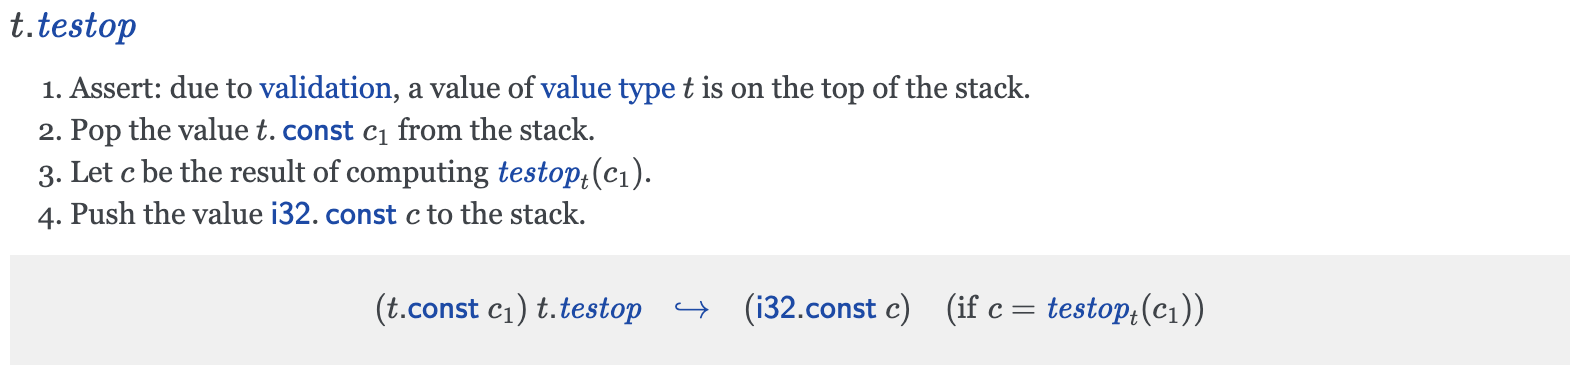
\includegraphics[width=15cm]{fig/testop}}
    \caption[\texttt{testop} instruction in official specification document]
      {\texttt{testop} instruction in official specification document}
      \label{fig:testop}
    \centerline{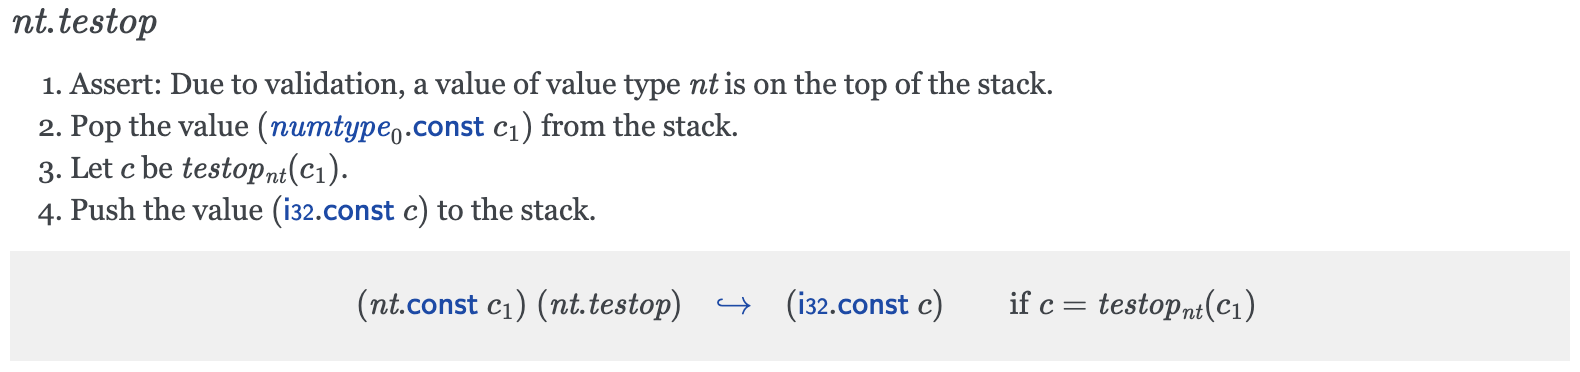
\includegraphics[width=15cm]{fig/spectec-testop}}
    \caption[\texttt{testop} instruction in SpecTec specification document]
      {\texttt{testop} instruction in SpecTec specification document}
      \label{fig:spectec-testop}
\end{figure}


% Challenging specification process
The demanding standardization process places a significant burden on
specification authors, particularly in maintaining consistency and correctness.
Crafting the specification document is labor-intensive, which becomes
increasingly difficult to scale as Wasm evolves.
This challenge is compounded by the dual requirement to maintain both a formal
notation, written in LaTeX, and a prose notation, authored in reStructuredText.
The separate and user-unfriendly nature of these formats hinders collaborative
review and increases the risk of discrepancies and errors between the two
notations, further complicating the standardization process.

% SpecTec
To mitigate this problem, we propose SpecTec~\cite{spectec}, a framework for
mechanizing WebAssembly specification.
It provides domain specific language (DSL) that enables the declarative
definition of Wasm syntax and semantics, akin to the formal notation.
SpecTec performs type-checking on the DSL to prevent meta-level specification
errors and generates LaTeX for the formal notation.
Additionally, to capture the pseudocode-like structure of the prose notation,
SpecTec incorporates an imperative language, \textit{AL}, which stands for
Algorithmic Language.
SpecTec translates the DSL into AL and generate reStructuredText for the prose
notation.
\cref{fig:spectec-testop} is the specification document generated by the
SpecTec using the DSL and the AL.
The generated document closely resembles the official document except for some
minor notation changes and some missing hyperlinks.
One notable aspect of AL is that it is executable, meaning any specification
written in AL serves as a Wasm interpreter program.
By testing the Wasm interpreter program, we can check the correctness of the
specification.
This bridges the gap between formal specification and executable code.
Futhermore, SpecTec generates mechanized definitions for theorem provers.


% Challenge
One challenge of our approach is making AL executable.
Since the prose notation in the official specification is written in informal
pseudocode, the interpretation of the prose notation is not straightforward.
The naive implementation of AL interpreter produced incorrect results when
running Wasm official test suites, particularly those related to control flow.
Additionally, the absence of a formalized definition or formal semantics for AL
made it difficult to identify and address the fundamental issues in its design.
Since running tests is the primary method for assessing the correctness of the
specification, this limitation hindered the development of both the generated
interpreter and the specification itself.
This underscored the need for a more robust approach to formally define AL and
ensure its alignment with Wasm's complex semantics.


% Solution
To address this, we present a formal model for how AL describes Wasm control flow.
Using this model, we identify the underlying issues and the necessary changes
to improve it.
Based on these insight, we formalize AL's syntax and semantics to accurately
capture Wasm control flow.
We then implement an AL interpreter according to this formalization and
evaluate its correctness.
The interpreter successfully passes all tests in the Wasm official test suite,
as well as tests from proposals.


% TODO: cref
% Contribution
The contributions of this paper are as follows:
\begin{itemize}
  \item We propose a formal model for Wasm control flow in AL (\cref{ch:motivation})
  \item We formalize syntax and semantics of AL (\cref{ch:formal})
  \item We implement an AL interpreter based on the formalization (\cref{ch:eval})
\end{itemize}


% !TEX root = main.tex

\chapter{Background}
\label{ch:background}
\noindent

\red{TODO: fix fig name}


\section{WebAssembly}
\label{sec:webassembly}


% breif overview
WebAssembly~\cite{wasm} is a low-level bytecode language that is safe, fast,
portable, and compact.
It is widely used as a compile target for web applications.
Not only that, other areas such as edge computing~\cite{wasm-edge},
IoT~\cite{wasm-iot}, and block chains~\cite{wasm-block} deploy the advantages
of WebAssembly.


% risk of implementation divergence
There are dozens of WebAssembly engines; all the browsers have there own
implementations of WebAssembly with multiple tiers ~\cite{v8}
\cite{spidermonkey} \cite{webkit}, and there are many engines that target for
specific areas including embedded systems and edge computing.
However, as WebAssembly should be portable across these implementations, it risks
the implementations divergence.


% rigorous standardization -> spec is rigorous: formal notation & prose notation
To mitigate this problem, WebAssembly has been standardized very rigourously by
the W3C~\cite{wasm-w3c}.
Especially, WebAssembly specification document is written very rigorously.
It describes the semantics of WebAssembly in two forms: formal notation and
prose notation.
Formal notation uses mathematical rules to compactly describe the semantics,
and it is used for proofs such as type soundness.
On the other hand, prose notation uses psudocodes algorithm to explain the
semantics through a step by step instruction.
Most WebAssembly users and engine developers are not familiar with
mathematical rules, so they utilize the prose notation.


% structure
A WebAssembly program is comprised of \textit{modules}.
A module is the unit of deployment, loading, and compilation, which consists of
definitions such as functions, globals, and memories.
A module is instantiated to validate the module and allocate each definition to
the data structure named \textit{store}.
This results in a module instance, a runtime representation for the module.
After the instantiation, functions can be invoked so that the function body,
which is a sequence of instructions, is executed.


% execution
WebAssembly execution is based on a stack machine.
An instruction consumes values in the stack as operands, performs some
operation, produces resulting values, and pushes them to the stack.
\cref{fig:testop} is the WebAssembly specification document for the
\texttt{testop} instruction.
Prose notation is written in the upper part, and formal notation is written in
the lower grey box.
In the prose notation, it pops a value from the stack, performs a test
operation, and pushes the result to the stack.
It is written compactly in the form of reduction rule in the formal notation
which consists of LHS, RHS, and premises: $(t.const ~ c_1) ~ t.testop$,
$(i32.const ~ c)$, and $c = testop_t(c_1)$.
The LHS means that the value at the top of the stack is $(t.const ~ c_1)$,
and an instruction to execute is $t.testop$.
The RHS means that the value at the top of the stack is changed to $(i32.const
~ c)$, and this happens when the premise $c = testop_t(c_1)$ is satisfied.


% control structure
The stack stores not only the input and output values of the instructions but also
structures related to the control flow.
A \textit{call frame} and a \textit{label} are used for function call and
branching, respectively.
In exception handling proposal, there is a \textit{handler} for exception
handling, and other strucutres could be introduced in the future.
How these control structures are used for the control flow will be discussed in
\cref{sec:control flow in official prose}.



\newcommand{\officialp}{official prose}
\newcommand{\spectecp}{SpecTec prose}

\red{TODO: explanation of the terms \officialp{} and \spectecp{}} \\
\red{TODO: remove redundant part in the fig} \\
\red{TODO: explanation of context(frame/label): in the background? or here?} \\
\red{TODO: the notion of meta-level interpreter in background} \\
\red{TODO: try finding better terminology rather than "model"} \\

\section{Control flow in official prose}
\label{sec:control flow in official prose}

% control flow structure in official prose
It might be easy to understand how the \officialp{} explains the control flow
of WebAssembly, if we assume that a WebAssembly code is loaded on a memory and
a pc points to the instruction to execute.
To describe control flow, it uses a structure named \textit{block} which
consitutes of a instruction sequence.
When executing the instructions in the block, pc can be changed to the starting
point of the block or the end of the block.


% an example of Wasm control flow in official prose
\begin{example}
\label{ex:br}
\begin{verbatim}
  // infinite loop
  (loop (result i32) (i32.const 42) (br 0) (unreachable) end) (unreachable)
\end{verbatim}
\end{example}

\cref{ex:br} is a WebAssembly code example that has \texttt{loop} and
\texttt{unreachable}
Here, result type of the \texttt{loop} is \texttt{i32} and the \texttt{loop}
has a block of three instructions: \texttt{i32.const}, \texttt{br}, and
\texttt{unreachable}.
\cref{fig:loop} is the \officialp{} of the \texttt{loop} instruction.
It says that the continuation is the start of the loop, the information is
stored in a label, and it \textit{enters} the block with the label.
The term \textit{enter} means that it pushes the label in the stack and makes
pc points to the first instruction in the block.
The \texttt{i32.const} instruction is executed first, which just pushes the
\texttt{i32} value \texttt{42} in the stack.
Then, The \texttt{br} instruction is executed.
\cref{fig:br} is the \officialp{} of the \texttt{br} instruction.
It pops the label from the stack, and makes pc points to the continuation of
the label, which is the start of the loop instruction.
As a result, the code example above is a infinite loop pushing \texttt{42}
forever without executing \texttt{unreachable} instructions.

\begin{figure}[h!]
    \centerline{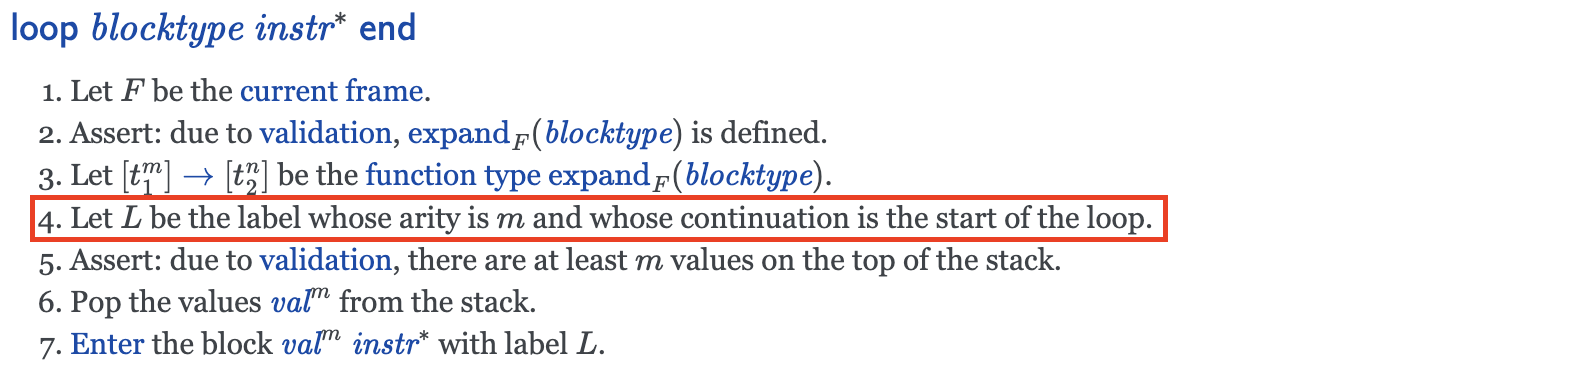
\includegraphics[width=15cm]{fig/loop}}
    \caption[Enter the caption title here]{\texttt{loop} instruction} \label{fig:loop}
    \centerline{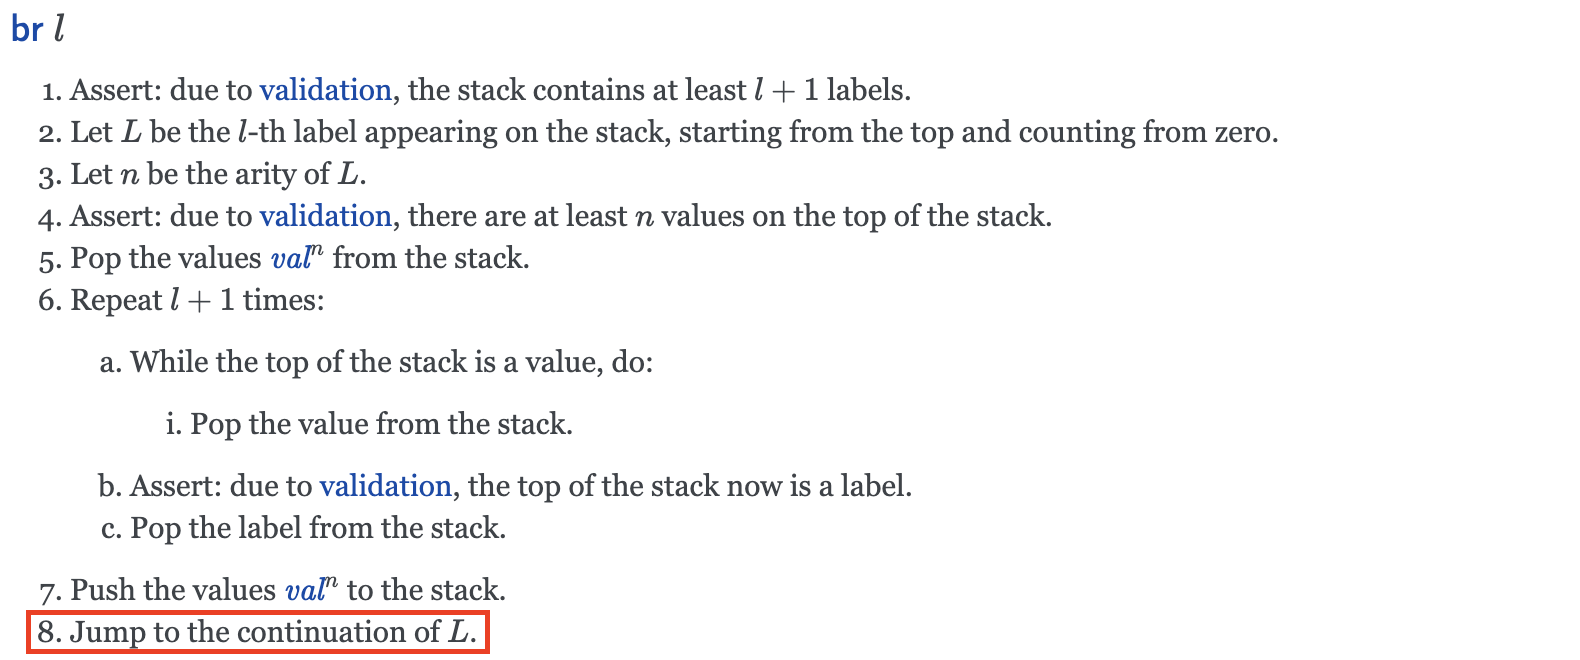
\includegraphics[width=15cm]{fig/br}}
    \caption[Enter the caption title here]{\texttt{br} instruction} \label{fig:br}
\end{figure}


% exiting label in official prose
There is also a special form of a behavior related to the block: an
\textit{exiting label}.
\cref{fig:exiting-label} is the \officialp{} of the \textit{exiting label}.
It is special because this behavior is performed without an explicit
WebAssembly instruction.
Rather, the behavior is performed when \textbf{the end of a block is reached}
without control instructions or runtime error.
The behavior is that the label is popped from the stack, and the pc changes to
the point after the end of the block.

\begin{figure}[h!]
    \centerline{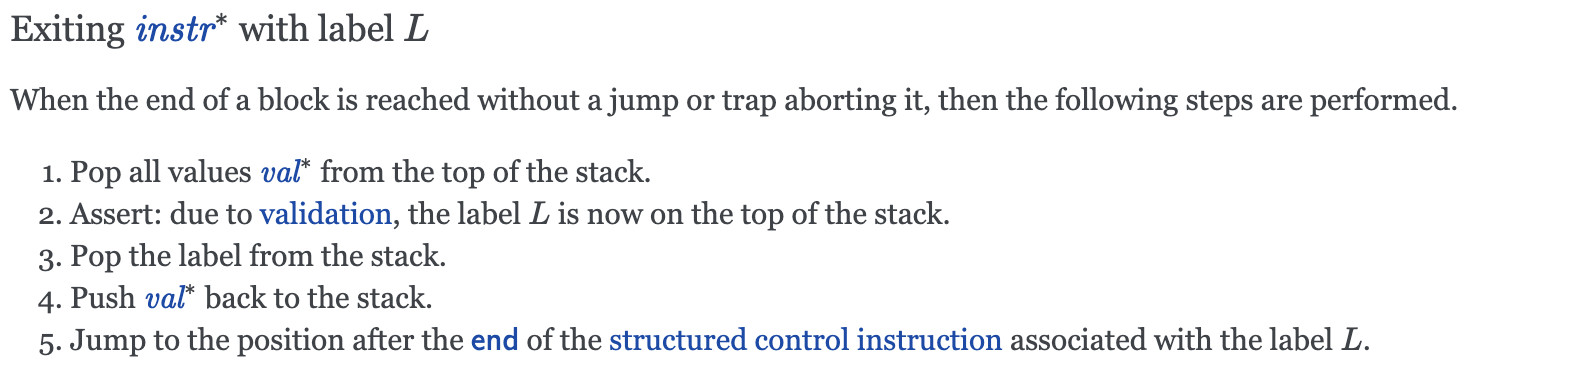
\includegraphics[width=15cm]{fig/exiting}}
    \caption[Enter the caption title here]{exiting label} \label{fig:exiting-label}
\end{figure}


% an example of exiting label in official prose
\begin{example}
\label{ex:exit}
\begin{verbatim}
  // exiting label
  (loop (result i32) (i32.const 42) end) (f64.const 3.14)
\end{verbatim}
\end{example}

\cref{ex:exit} is a WebAssembly code example that has \texttt{loop} whose block is
only \texttt{i32.const}, and \texttt{f32.const}
When the \texttt{loop} instruction is executed, it enters the block with a label.
After \texttt{i32.const} is executed, the end of the block is reached.
As a result, exiting label occurs so that the label is popped from the stack,
pc changes to the point after the end of block: \texttt{f64.const}.
As a result, after executing the code, the value 42 and 3.14 pushed to the
stack.


% control flow structure with function call in official prose
Similar to the control flow using the block and the label, there is a function
call with a frame.
\cref{fig:invoke} is the \officialp{} of the function invocation which takes
place by a \texttt{call} instruction.
A frame is pushed to the stack and enters the block of the function body with a
label.
There is also a special behavior named returning from a function.
\cref{fig:returning} is the \officialp{} of the returning from a function.
When end of function is reached without without control instructions or runtime
error, The frame is popped from the stack, and the pc points to the next
instruction of the caller instruction.

\begin{figure}[h!]
    \centerline{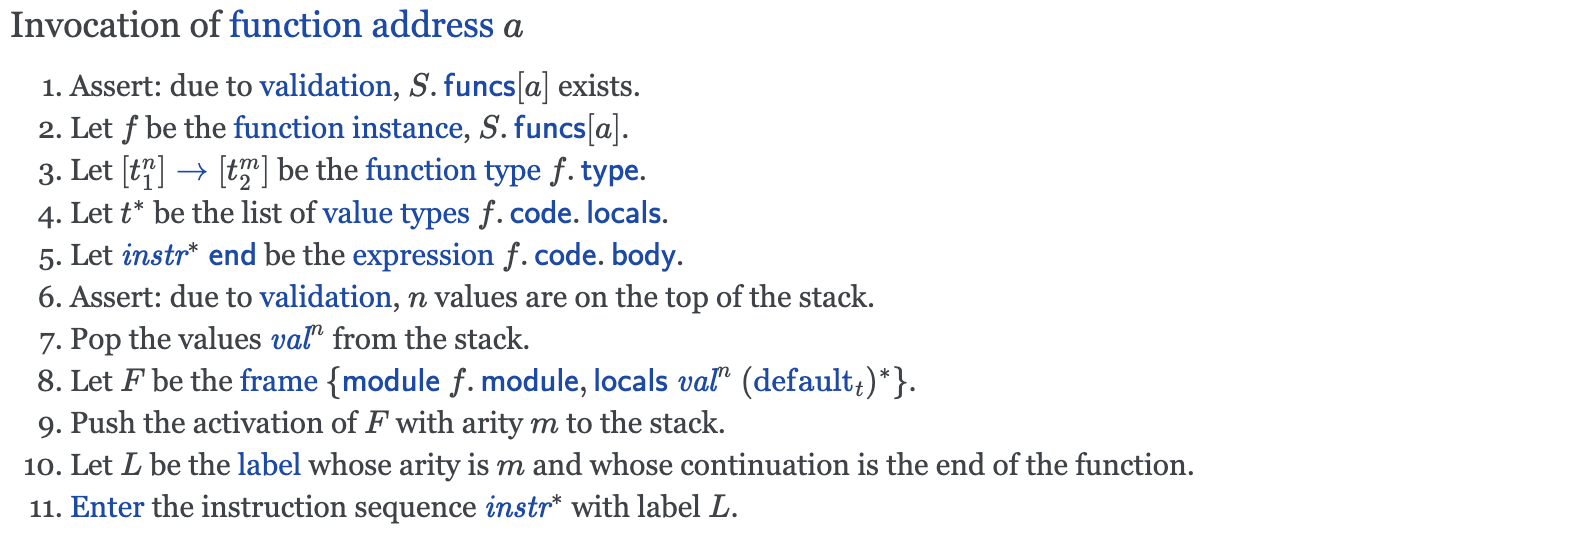
\includegraphics[width=15cm]{fig/invoke}}
    \caption[Enter the caption title here]{function invocation} \label{fig:invoke}
    \centerline{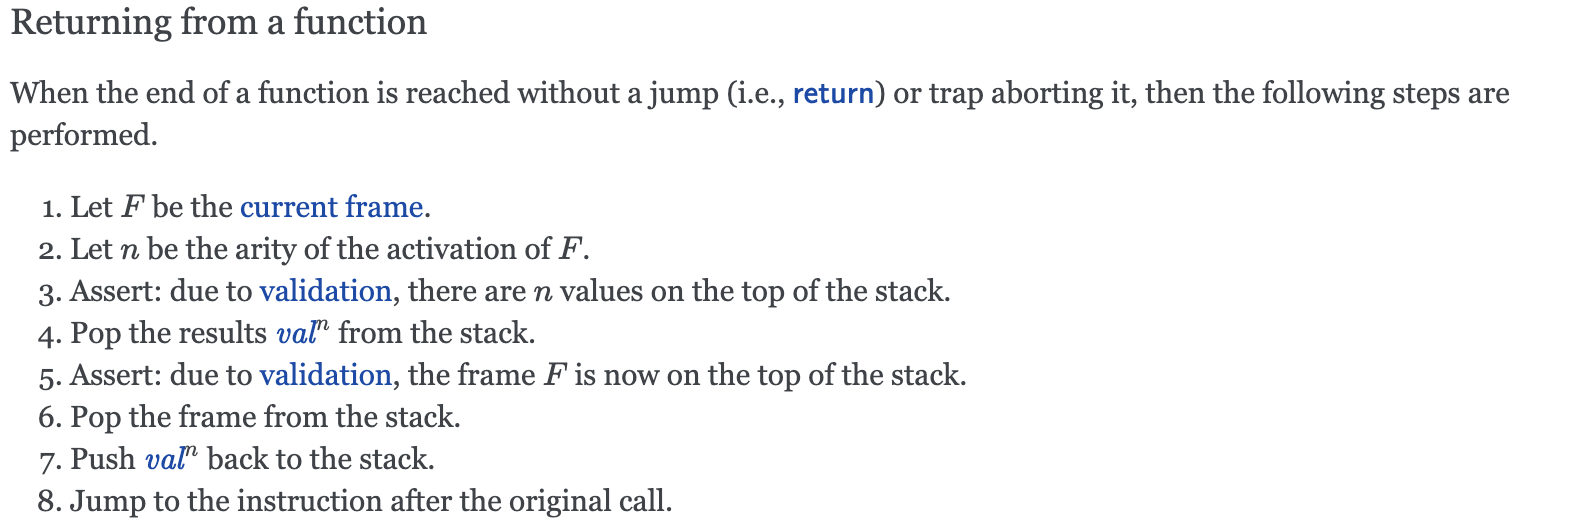
\includegraphics[width=15cm]{fig/returning}}
    \caption[Enter the caption title here]{returning from a function} \label{fig:returning}
\end{figure}



% !TEX root = main.tex

\chapter{Motivation}
\label{ch:motivation}
\noindent

\newcommand{\officialp}{official prose}
\newcommand{\spectecp}{SpecTec prose}

\red{TODO: explanation of the terms \officialp{} and \spectecp{}} \\
\red{TODO: remove redundant part in the fig} \\
\red{TODO: explanation of context(frame/label): in the background? or here?} \\
\red{TODO: the notion of meta-level interpreter in background} \\
\red{TODO: try finding better terminology rather than "model"} \\


\section{Control flow in official prose}
\label{sec:control flow in official prose}

% control flow structure in official prose
It might be easy to understand how the \officialp{} explains the control flow
of WebAssembly, if we assume that a WebAssembly code is loaded on a memory and
a pc points to the instruction to execute.
To describe control flow, it uses a structure named \textit{block} which
consitutes of a instruction sequence.
When executing the instructions in the block, pc can be changed to the starting
point of the block or the end of the block.


% an example of Wasm control flow in official prose
\begin{example}
\label{ex:br}
\begin{verbatim}
  // infinite loop
  (loop (result i32) (i32.const 42) (br 0) (unreachable) end) (unreachable)
\end{verbatim}
\end{example}

\cref{ex:br} is a WebAssembly code example that has \texttt{loop} and
\texttt{unreachable}
Here, result type of the \texttt{loop} is \texttt{i32} and the \texttt{loop}
has a block of three instructions: \texttt{i32.const}, \texttt{br}, and
\texttt{unreachable}.
\cref{fig:loop} is the \officialp{} of the \texttt{loop} instruction.
It says that the continuation is the start of the loop, the information is
stored in a label, and it \textit{enters} the block with the label.
The term \textit{enter} means that it pushes the label in the stack and makes
pc points to the first instruction in the block.
The \texttt{i32.const} instruction is executed first, which just pushes the
\texttt{i32} value \texttt{42} in the stack.
Then, The \texttt{br} instruction is executed.
\cref{fig:br} is the \officialp{} of the \texttt{br} instruction.
It pops the label from the stack, and makes pc points to the continuation of
the label, which is the start of the loop instruction.
As a result, the code example above is a infinite loop pushing \texttt{42}
forever without executing \texttt{unreachable} instructions.

\begin{figure}[h!]
    \centerline{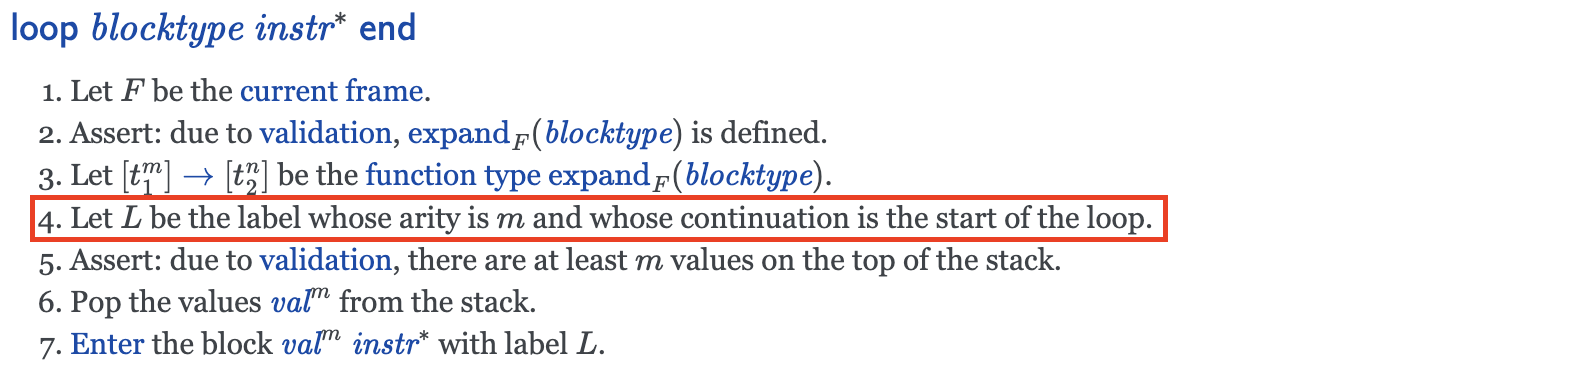
\includegraphics[width=15cm]{fig/loop}}
    \caption[Enter the caption title here]{\texttt{loop} instruction} \label{fig:loop}
    \centerline{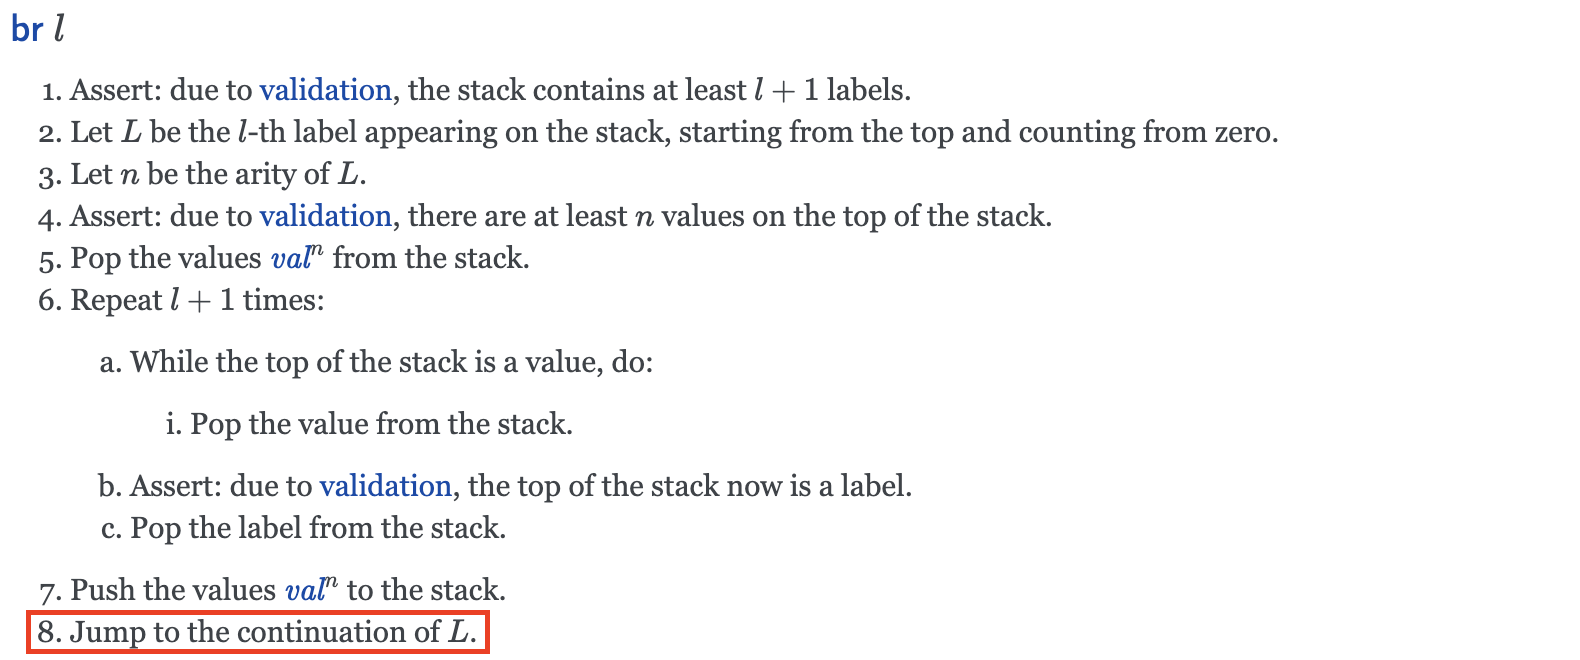
\includegraphics[width=15cm]{fig/br}}
    \caption[Enter the caption title here]{\texttt{br} instruction} \label{fig:br}
\end{figure}


% exiting label in official prose
There is also a special form of a behavior related to the block: an
\textit{exiting label}.
\cref{fig:exiting-label} is the \officialp{} of the \textit{exiting label}.
It is special because this behavior is performed without an explicit
WebAssembly instruction.
Rather, the behavior is performed when \textbf{the end of a block is reached}
without control instructions or runtime error.
The behavior is that the label is popped from the stack, and the pc changes to
the point after the end of the block.

\begin{figure}[h!]
    \centerline{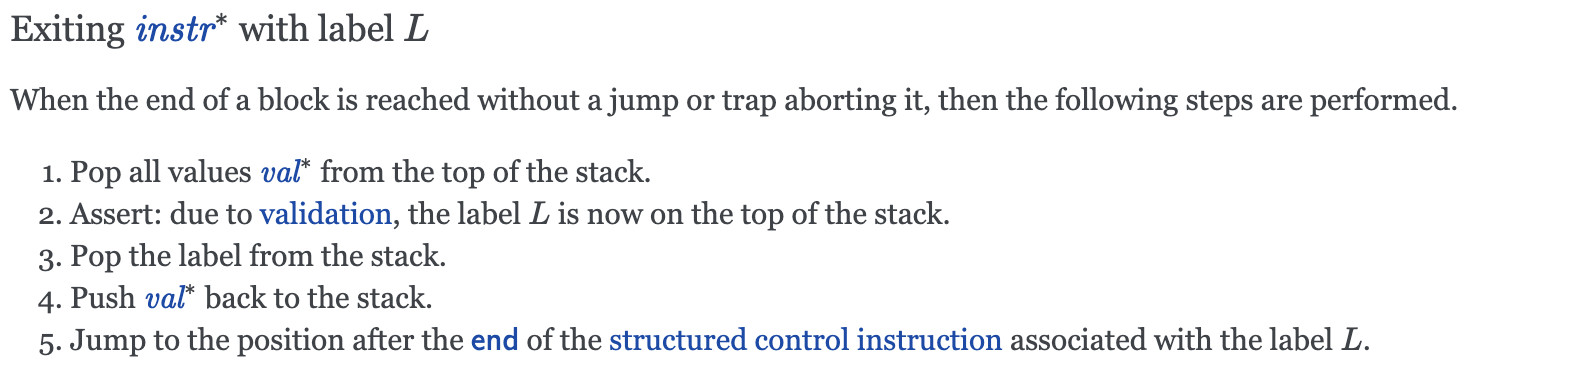
\includegraphics[width=15cm]{fig/exiting}}
    \caption[Enter the caption title here]{exiting label} \label{fig:exiting-label}
\end{figure}


% an example of exiting label in official prose
\begin{example}
\label{ex:exit}
\begin{verbatim}
  // exiting label
  (loop (result i32) (i32.const 42) end) (f64.const 3.14)
\end{verbatim}
\end{example}

\cref{ex:exit} is a WebAssembly code example that has \texttt{loop} whose block is
only \texttt{i32.const}, and \texttt{f32.const}
When the \texttt{loop} instruction is executed, it enters the block with a label.
After \texttt{i32.const} is executed, the end of the block is reached.
As a result, exiting label occurs so that the label is popped from the stack,
pc changes to the point after the end of block: \texttt{f64.const}.
As a result, after executing the code, the value 42 and 3.14 pushed to the
stack.


% control flow structure with function call in official prose
Similar to the control flow using the block and the label, there is a function
call with a frame.
\cref{fig:invoke} is the \officialp{} of the function invocation which takes
place by a \texttt{call} instruction.
A frame is pushed to the stack and enters the block of the function body with a
label.
There is also a special behavior named returning from a function.
\cref{fig:returning} is the \officialp{} of the returning from a function.
When end of function is reached without without control instructions or runtime
error, The frame is popped from the stack, and the pc points to the next
instruction of the caller instruction.

\begin{figure}[h!]
    \centerline{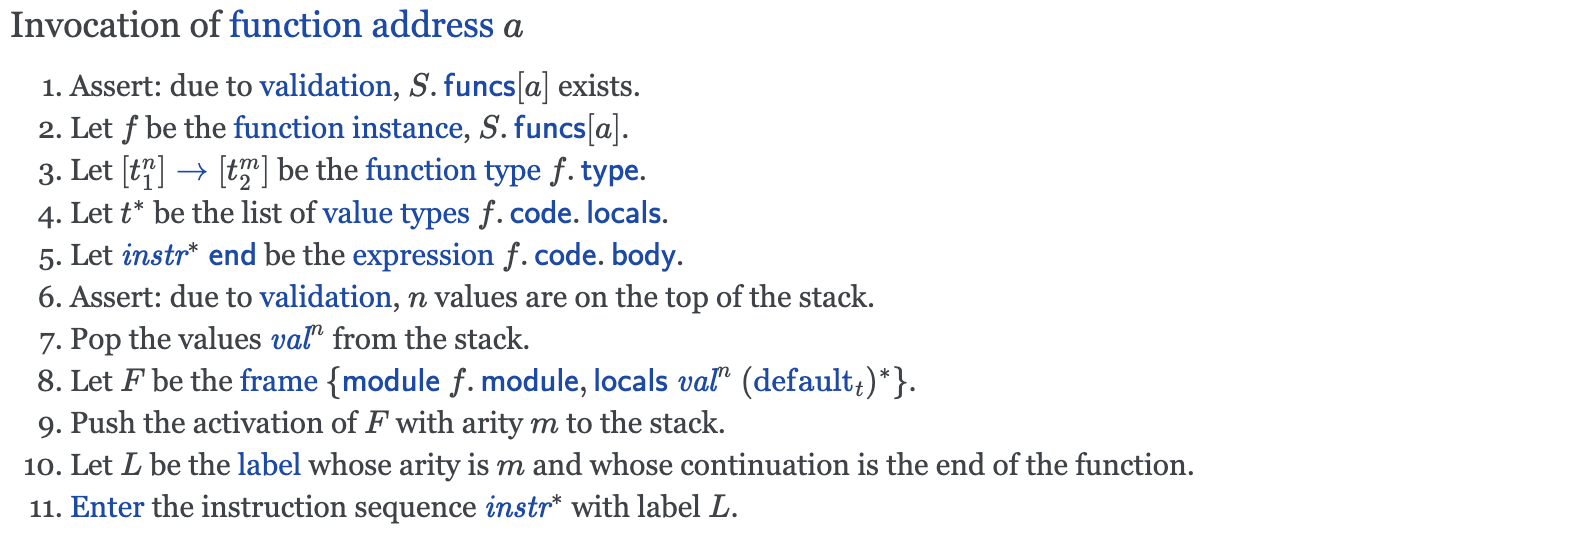
\includegraphics[width=15cm]{fig/invoke}}
    \caption[Enter the caption title here]{function invocation} \label{fig:invoke}
    \centerline{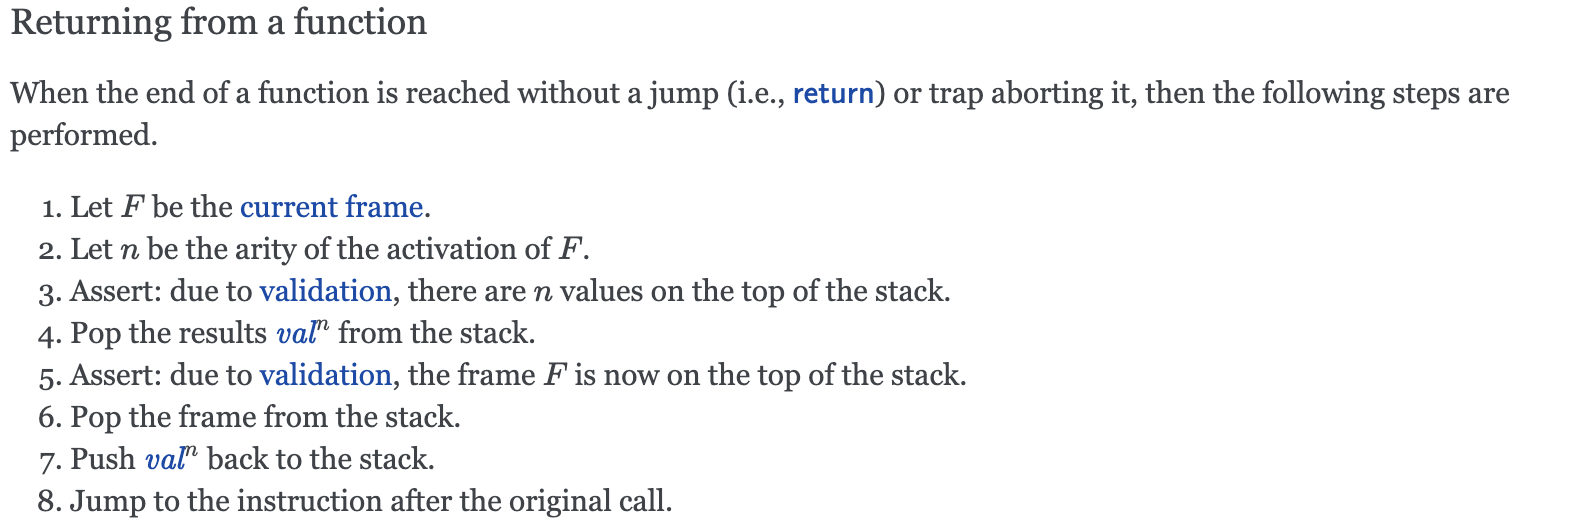
\includegraphics[width=15cm]{fig/returning}}
    \caption[Enter the caption title here]{returning from a function} \label{fig:returning}
\end{figure}

\section{Control flow in SpecTec prose}
\label{sec:spectecp}

% control flow structure in SpecTec prose
However, the \spectecp{} assumes a different model to explain the control flow
of WebAssembly.
Rather than using the notion of a pc, \spectecp{} assumes that WebAssembly
instructions are just given one by one.
This is because the \spectecp{} is generated automatically from the
\red{SpecTec DSL}.
\red{SpecTec DSL} uses rewrite rule to describe WebAssembly semantics, and it
is interpreted in \spectecp{} as consuming a WebAssembly instruction, pushing
or poping a control structures, and inputing new WebAssembly instructions.
It can be expressed in the following form:
$c^* \vdash i_0, i_1, ..., i_m \leadsto c'^* \vdash i'_0, ...i'_{m'}, i_1, ..., i_m$.
It means that given a sequence of contexts $c^*$, executing $i_0$ results in a
new sequence of contexts $c'^*$ and instructions $i'_0, ...i'_{m'}$.
To simply model the control flow of WebAssembly, other things not closely
related to the control flow are omitted in this notation.


% challenges in SpecTec prose
However, this viewpoint is challenged by the exiting label.
As the block structure doesn't remain intact in this model, it is hard to
describe \textbf{the end of the block}.
Furthermore, the exiting label is not performed by a specific WebAssembly
instruction, which makes it hard to model the behavior.
To handle this problem, an administrative instruction \texttt{end} is
introduced in \spectecp.
When entering a block, an \texttt{end} is appended to the end of the block.


% an example of Wasm control flow in official prose
\begin{figure}[h!]
    \centerline{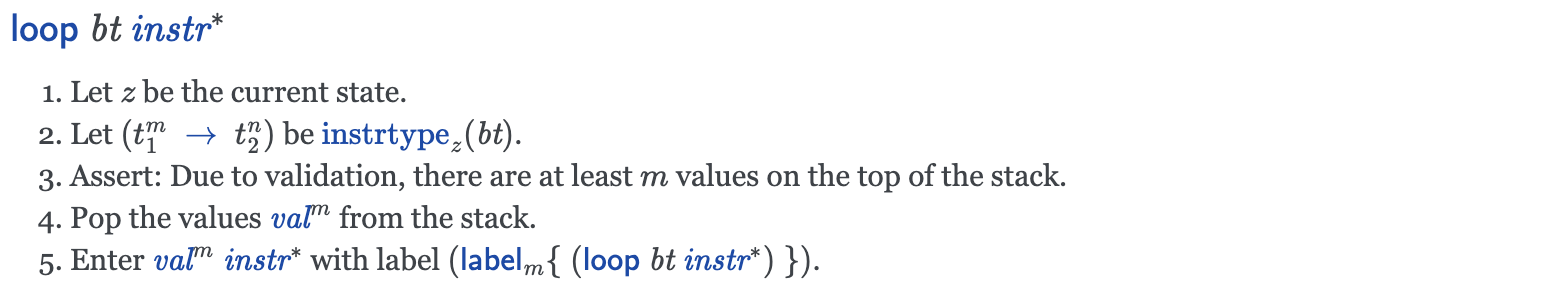
\includegraphics[width=15cm]{fig/spectec-loop}}
    \caption[Enter the caption title here]{SpecTec \texttt{loop}} \label{fig:spectec-loop}
\end{figure}
\begin{figure}[h!]
    \centerline{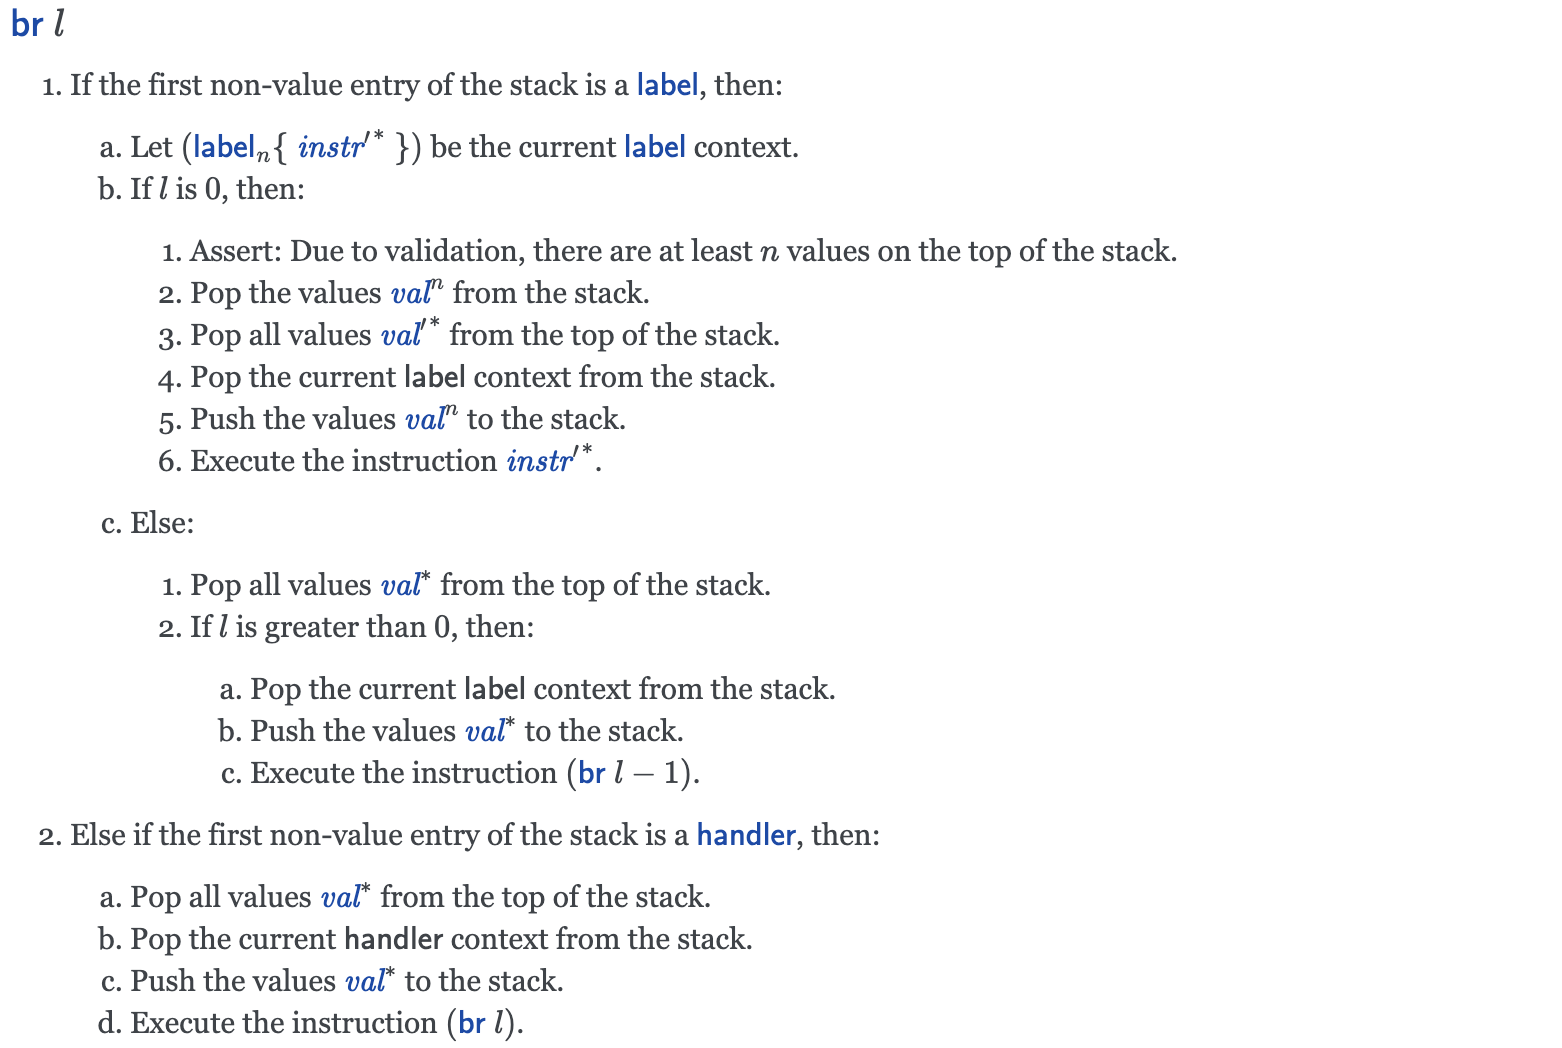
\includegraphics[width=15cm]{fig/spectec-br}}
    \caption[Enter the caption title here]{SpecTec \texttt{br}} \label{fig:spectec-br}
\end{figure}

\red{TODO: Change to array} \\
\begin{align}
  &c^*
  \vdash
  loop([ ~ i32.const ~ 42, ~ br ~ 0, ~ unreachable ~ ]), ~ unreachable
  \label{eq:loop-1} \\
&\leadsto
  label(loop([ ~ i32.const ~ 42; ~ br ~ 0; ~ unreachable ~ ])), c^*
  \vdash
  i32.const ~ 42, ~ br ~ 0, ~ unreachable, ~ end, ~ unreachable
  \label{eq:loop-2} \\
  &\leadsto
  label(loop([ ~ i32.const ~ 42; ~ br ~ 0; ~ unreachable ~ ])), c^*
  \vdash
  ~ br ~ 0, ~ unreachable, ~ end, ~ unreachable
  \label{eq:loop-3} \\
&\leadsto
  c^*
  \vdash
  loop([ ~ i32.const ~ 42; ~ br ~ 0; ~ unreachable ~ ]), unreachable
  \label{eq:loop-4}
\end{align}

Consider \cref{ex:br} above.
If we assume some control structure $c^*$ is given, the code can be expressed
like \cref{eq:loop-1}.
\cref{fig:spectec-loop} is the \spectecp{} of the \texttt{loop} instruction.
Rather than storing the point to jump as a continuation in the label, it stores
the \texttt{loop} instruction itself in the label, and \textit{enters} the
block.
Here, \textit{enter} means that it pushes the label in the stack and executes
the instructions in the block, which means that \texttt{i32.const},
\texttt{br}, \texttt{unreachable}, \texttt{end} and \texttt{unreachable} become
the new inputs in \cref{eq:loop-2}.
When \texttt{i32.const} is excuted, it pushes 42 as \officialp{} does
in \cref{eq:loop-3}.
The value is omitted for brevity.
However, \texttt{br} behaves a bit differently.
\cref{fig:spectec-br} is the \spectecp{} of the \texttt{br} instruction.
It pops the label from the stack, removes the input instructions until the end
of the block including the \texttt{end}, considers the loop instruction in the
label as a new input instruction.
Consequently, remaining inputs are \texttt{loop}, and \texttt{unreachable}
again in \cref{eq:loop-4}.
Therefore, it explains the same behavior in a different point of view.

\red{TODO: Also use example 3 to explain function call in official prose}

% an example of function call in official prose
\begin{example}
\label{ex:invoke}
\begin{verbatim}
  // function definition of $push42
  (func $push42 (result i32) (i32.const 42))

  // function call
  (call $push42) (f32.const 3.14)
\end{verbatim}
\end{example}

\red{TODO: Change to array} \\
\begin{align}
  &c^* \vdash call(\$push42), ~ f32.const ~ 3.14 \label{eq:call-1} \\
&\leadsto
  Label(\epsilon), ~ Frame, ~ c^* \vdash i32.const ~ 42, ~ end, ~ f32.const ~ 3.14 \label{eq:call-2} \\
&\leadsto
  Label(\epsilon), ~ Frame, ~ c^* \vdash end, ~ f32.const ~ 3.14 \label{eq:call-3} \\
&\leadsto
  c^* \vdash f32.const ~ 3.14 \label{eq:call-4} \\
&\leadsto
  c^* \vdash \epsilon \label{eq:call-5}
\end{align}

\cref{ex:invoke} contains a function definition whose body is \texttt{i32.const}, a
\texttt{call} instruction followed by a \texttt{f32.const} instruction, which
can be expressed in \cref{eq:call-1}.
By invoking a function, it pushes a frame and enters the block with a label in
\cref{eq:call-2}.
After executing the body in \cref{eq:call-3}, an \texttt{end} is executed.
In this point, this \texttt{end} represent both the end of the block and the
function.
As a consequence, this \text{end} perform both exiting label and returning from
a function in \cref{eq:call-4}, and the instruction after the \texttt{call} is
executed in \cref{eq:call-5}
It results in the values 42 and 3.14 pushed to the stack.


% summary & test
In short, the behavior of an \texttt{end} instruction 1) performs exiting
label, 2) looks up the top of the context, and 3) performs returing from a
function, if it is a frame.
The \spectecp{} can model the WebAssembly control flow using this \texttt{end}
instruction.
To show the correctness of the \spectecp{}, we run the WebAssembly tests
including official WebAssembly test suite by executing the \spectecp{} with
\red{definitional interpreter}.


% Problem
However, tests related to the control instruction are failed.
At that time, there was no explicit model to describe the control flow in
\spectecp{}, it was hard to define the problem, making it complicated to fix
the problem.



%%%%%%%%

% an example of buggy test case
\begin{example}
\label{ex:bug}
\begin{verbatim}
  // function definition of $br-returning
  (func  $brAndReturning (br 0) (unreachable))

  // function call
  (call $brAndReturning)
\end{verbatim}
\end{example}

\cref{ex:bug} contains a function that has only a \texttt{br} instruction, and a
\texttt{call} insstruction.
According to the \officialp{}, when the function \texttt{\$brAndReturning} is
called, a frame is pushed to the stack, and the block of the function
body is entered with a label.
When the \texttt{br} is executed, it pops the label from the stack.
As the end of the function is reached after the execution, returning from a
function is performed.
As a result, the frame is popped, so the call actually does nothing.


% explaination of the bug in SpecTec prose
\begin{align}
  &c^* \vdash call(\$brAndReturning) \label{eq:bug-1} \\
&\leadsto
  Label(\epsilon), ~ Frame, ~ c^* \vdash (br ~ 0) ~ (unreachable), ~ end \label{eq:bug-2} \\
&\leadsto
  Frame, ~ c^* \vdash \epsilon \label{eq:bug-3}
\end{align}

In \spectecp{} the call instruction in \cref{eq:bug-1} pushes a frame and
enters the function body \cref{eq:bug-2}.
When the \texttt{br} is executed, it pops the label and removes the input
instructions until the end in \cref{eq:bug-3}.
As a result, the frame is remained after the executing the call.
The problem is that the \texttt{br} should remove the end of the block but
should not remove the end of the function, but \texttt{end} express the end of
the block and the function at the same time.


% Fix
To fix the problem, semantics of \enteri is changed.
The sequence of contexts that is pushed in the AL algorithm is stored,
and when a block is entered, exiting label and returning from a function is
appended according to the sequence.




% !TEX root = main.tex

\chapter{Overview}
\label{ch:overview}
\noindent


\begin{figure}[t]
  \centerline{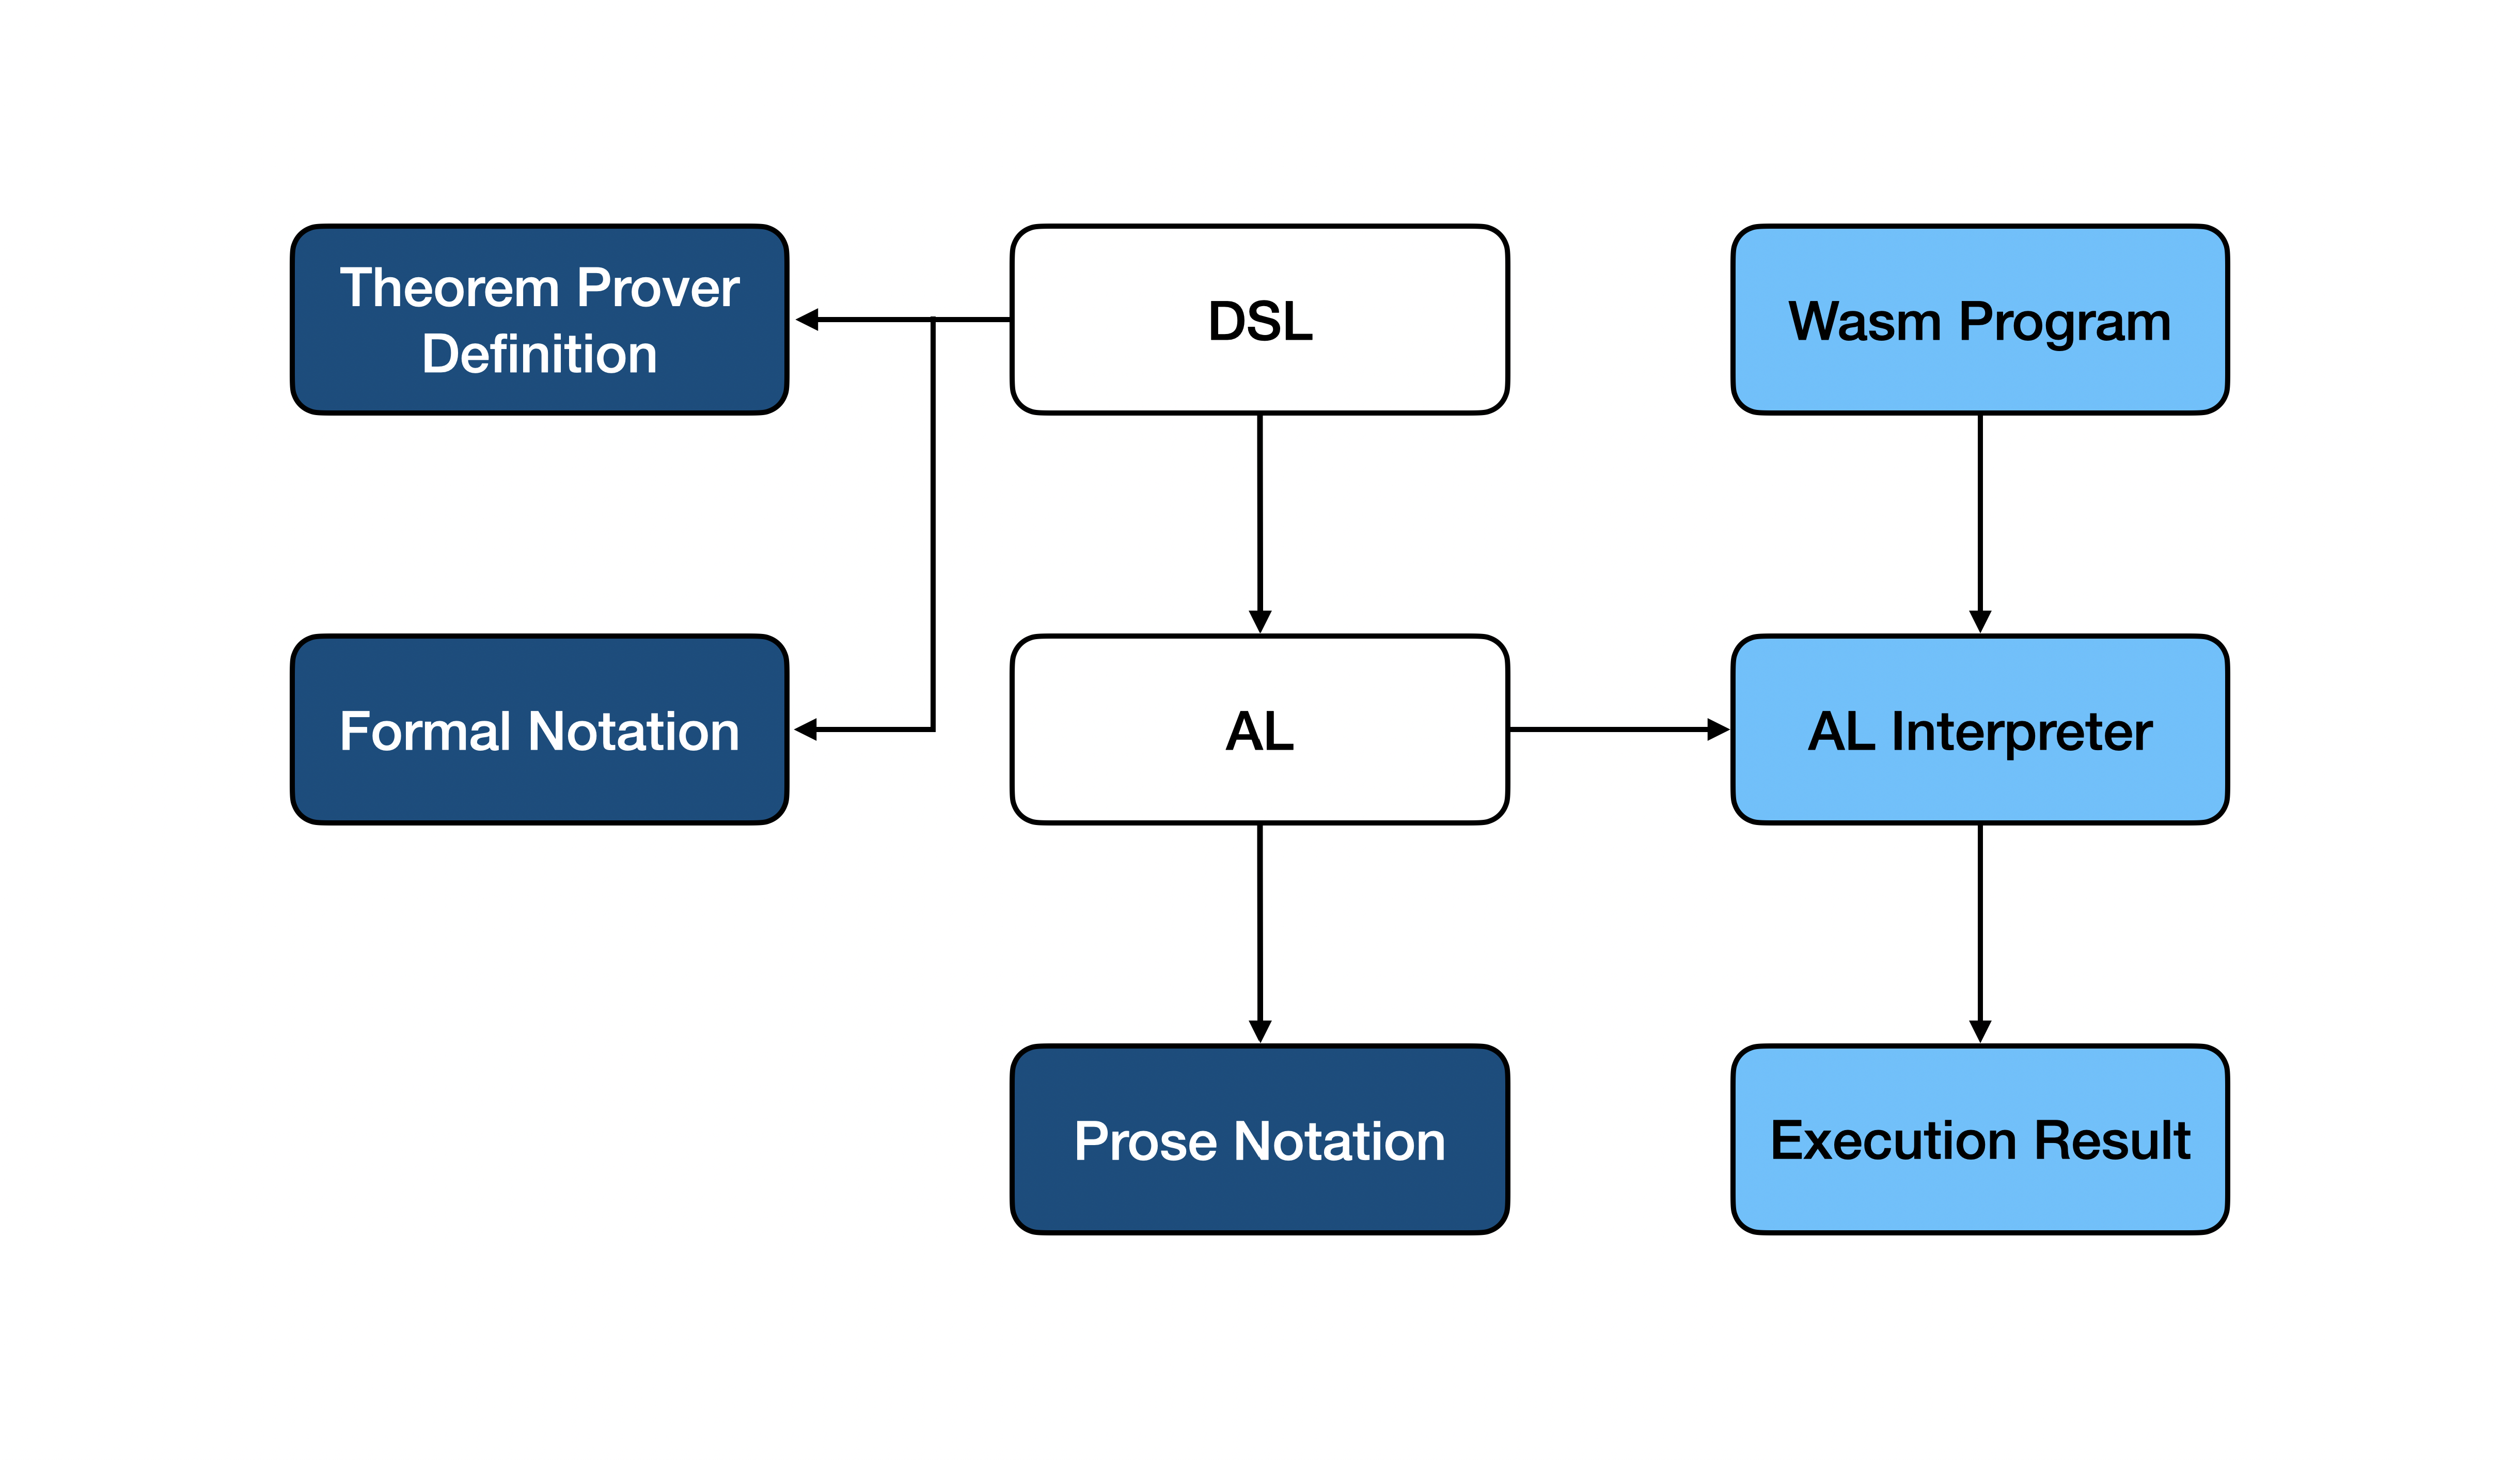
\includegraphics[width=15cm]{fig/overview}}
  \caption[An overview of the SpecTec architecture]
    {An overview of the SpecTec architecture}
    \label{fig:overview}
\end{figure}

% SpecTec: specification mechanization tool
SpecTec is a tool for \textit{mechanizing} WebAssembly specification
~\cite{spectec}.
Specification mechanization is a technique that treats a specification as data
that can be manipulated by a machine to automatically generate parser and
interpreter ~\cite{jiset}, to generate tests and perform differential tests
~\cite{jest}, to find meta-level errors in the specification ~\cite{jstar}, and
to perform meta-level static analysis for the static analysis of the defined
language ~\cite{jsaver}.
% Overview explanation
In this chapter, we explain the overall approach to generating multiple
artifacts from the specification and ensuring the correctness of the
specification.
\Cref{fig:overview} illustrates an overview of our approach.


% DSL
SpecTec offers a domain specific language (DSL) designed for writing
Wasm specifications.
It is a declarative language, providing a compact and user-friendly syntax.
This DSL can represent Wasm semantics in a manner closely resembling the formal
notation as shown in the following code for specification of testop
instruction.
The code below shows the specification for the \texttt{testop} instruction
written in the DSL:
\begin{lstlisting}[style=dsl]
  rule Step_pure/testop:
  (CONST nt c_1) (TESTOP nt testop)  ~>  (CONST I32 c)
  -- if c = @\dollarcode@testop_(nt, testop, c_1)
\end{lstlisting}
The DSL is type checked to prevent meta-level errors such as notation misuses and
dimension mismatches.
Using the DSL, SpecTec generates LaTeX code and mechanized definitions for theorem provers.


% AL
Additionally, SpecTec introduces another imperative language, \textit{AL}, for
the prose notation.
In AL, semantics are expressed algorithmically, in the form of step-by-step
instructions that take inputs and perform operations, mirroring the prose notation.
SpecTec translates declarative definitions in the DSL into algorithmic
definitions in AL.
The AL code below is the specification for the \texttt{testop} instruction
generated from the DSL:
\begin{lstlisting}[style=al]
@\textbf{Step\_pure/testop}@ nt testop {
    Assert (check_type_of_stack_top(nt))
    Pop (CONST nt c_1)
    Let c = @$\dollarcode$@testop_(nt, testop, c_1)
    Push (CONST I32 c)
}
\end{lstlisting}
Using AL, SpecTec generates reStructuredText code.
\cref{fig:spectec-testop} shows the generated document for \texttt{testop}
instruction.
The generated document closely resembles the official document except for some
minor notation changes and some missing hyperlinks.


% AL interpreter
A notable feature of AL is that it is interpretable.
SpecTec includes an AL interpreter that executes an AL program with given inputs
and produces results.
Since an AL program specify the behavior of a Wasm program, the input to an AL
program is a Wasm program, and the result is the execution outcome of the Wasm
program.
In other words, the generated AL program functions as a WebAssembly interpreter.
What is particularly intriguing is that if specification authors write a Wasm
specification using the DSL, a WebAssembly interpreter that adheres to the
defined semantics is automatically generated.
By testing this generated interpreter, we can assess the specification,
thereby ensuring its correctness.


% !TEX root = main.tex

\chapter{SpecTec}
\label{ch:spectec}
\noindent



\newcommand{\seq}[1]{#1^*}







\section{SpecTec}
\label{sec:spectec}


% SpecTec: specification mechanization tool
SpecTec is a tool for \textit{mechanizing} WebAssembly specification
~\cite{spectec}.
Specification mechanization is a technique that treats a specification as data
that can be manipulated by a computer to automatically generate parser and
interpreter ~\cite{jiset}, to generate tests and perform differential tests
~\cite{jest}, to find meta-level errors in the specification ~\cite{jstar}, and
to perform meta-level static analysis for the static analysis of the defined
language ~\cite{jsaver}.
This technique is especially crucial in growing languages such as JavaScript
and WebAssembly.


% DSL high-level explanation
SpecTec provides a domain specific language (DSL) for the specification.
The DSL is a declarative language that resembles textbook style notation.
It is type checked to prevent meta-level errors such as notation misuses and
dimension mismatches. The code below is the specification for \texttt{testop}
instruction written in the DSL, which is designed to be similar to the formal
notation when describing the semantics with compact and user-friendly
notation.
\\
\red{TODO: better character for $\sim$ in the code}
\begin{verbatim}
  rule Step_pure/testop:
  (CONST nt c_1) (TESTOP nt testop)  ~>  (CONST I32 c)
  -- if c = $testop_(nt, testop, c_1)
\end{verbatim}


% DSL
The DSL consists of DSL definitions.
There are mainly 4 kinds of DSL definitions: type, grammar, relation, and
functions.
Type definitions are used to define abstract syntax, while grammar definitions
are used to define concrete syntax.
Relation definitions are used to define semantics; the code above is also
described in relation definition.
Function definitions can be utilized for other definitions such as
\texttt{\$testop\_} in the code.
In addition, they can be also used to describe semantics.
Especially, SpecTec uses function definitions to describe module instantiation
and function invocation.


% AL
However, The DSL cannot generate the prose notation just as it is because it is
declarative.
Therefore, SpecTec also defines another imperative language \textit{AL}, which
stands for algorithmic language, for the prose notation.
SpecTec translates the semantics describing part of the DSL, which is the
relation defintions and the function definitions, into the AL.
Both definitions are expressed in the form of algorithms in AL that takes some
inputs and performs a step by step instructions as in the prose notation.


% meta-level interpreter
What is especially intriguing here is that AL is executable.
It can perform each step written in the prose program one by one, which
WebAssembly interpreter should follow.
As a result, the prose program serves as a WebAssembly interpter.
That is to say, if WebAssembly semantics is written in the DSL, SpecTec
automatically generates the WebAssembly interpreter following the written
semantics.
The generated interpreter passes all the execution tests in the official test
suites except for the tests related to the infinte loop.


% artifacts SpecTec generates & SpecTec for other language
\cref{fig:spectec-testop} is the specification document generated by the
SpecTec using the DSL and the AL.
The generated document closely resembles the official document except for some
minor notation changes and some missing hyperlinks.
Additionally, SpecTec can generate many other artifacts automatically from the
DSL.
SpecTec translates the DSL into Coq for mathematical proofs and is working
on generating other artifacts, such as test suites required for WebAssembly
standardization.
Furthermore, research is ongoing to extend SpecTec for mechanizing other
languages ~\cite{p4-cherry-workshop}.



%% Syntax
\section{Syntax of AL}
\label{syntax}

{
\renewcommand{\arraystretch}{0.8835}  % Decrease row spacing locally
\begin{align*}
\begin{array}{lcccrlr}
%
% Algorithm
  \text{Algorithm}\quad& A &\ni& a &::=& ~ \rel ~ (s, \seq e, \seq i) ~ | ~ \fun ~ (s, \seq e, \seq i) \\
%
% Instruction
  \text{Instruction}\quad& I &\ni& i &::=& ~ \ifi ~ (e, \seq i, \seq i) &\quad\text{(If)} \\
    &&&& | & ~ \eitheri ~ (\seq i, \seq i) &\quad\text{(Either)} \\
    &&&& | & ~ \enteri ~ (e, e) &\quad\text{(Enter)} \\
    &&&& | & ~ \pushctxi ~ e &\quad\text{(Push Context)} \\
    &&&& | & ~ \pushi ~ e &\quad\text{(Push)} \\
    &&&& | & ~ \popctxi ~ e &\quad\text{(Pop Context)} \\
    &&&& | & ~ \popi ~ e &\quad\text{(Pop)} \\
    &&&& | & ~ \popni ~ (e, e) &\quad\text{(Pop N)} \\
    &&&& | & ~ \popalli ~ e &\quad\text{(Pop All)} \\
    &&&& | & ~ \leti ~ (e, e) &\quad\text{(Let)} \\
    &&&& | & ~ \trapi &\quad\text{(Trap)} \\
    &&&& | & ~ \returnreli &\quad\text{(Return Relation)} \\
    &&&& | & ~ \returnfuni ~ e &\quad\text{(Return Function)} \\
    &&&& | & ~ \executei ~ e &\quad\text{(Execute)} \\
    &&&& | & ~ \calli ~ (s, s, \seq{e}) &\quad\text{(Let Call)} \\
    &&&& | & ~ \replaceframei ~ (p^+, e) &\quad\text{(Replace Frame)} \\
    &&&& | & ~ \replacestorei ~ (p^+, e) &\quad\text{(Replace Store)} \\
%
% Expression
  \text{Expression}\quad& E &\ni& e &::=& ~ \vare ~ s &\quad\text{(Variable)} \\
    &&&& | & ~ \nume ~ n &\quad\text{(Number)} \\
    &&&& | & ~ \boole ~ b &\quad\text{(Boolean)} \\
    &&&& | & ~ \fnamee ~ s &\quad\text{(Function Name)} \\
    &&&& | & ~ \liste ~ \seq e &\quad\text{(List)} \\
    &&&& | & ~ \stre ~ \seq{(s, e)} &\quad\text{(Record)} \\
    &&&& | & ~ \tupe ~ \seq e &\quad\text{(Tuple)} \\
    &&&& | & ~ \casee ~ (s, \seq e) &\quad\text{(Tagged Tuple)} \\
    &&&& | & ~ \une ~ (unop, e) &\quad\text{(Unary Operation)} \\
    &&&& | & ~ \bine ~ (binop, e, e) &\quad\text{(Binary Operation)} \\
    &&&& | & ~ \acce ~ (e, p) &\quad\text{(Access)} \\
    &&&& | & ~ \upde ~ (e, p^+, e) &\quad\text{(Update)} \\
    &&&& | & ~ \cate ~ (e, e) &\quad\text{(Concatenation)} \\
    &&&& | & ~ \compe ~ (e, e) &\quad\text{(Composition)} \\
    &&&& | & ~ \meme ~ (e, e) &\quad\text{(Membership)} \\
    &&&& | & ~ \choosee ~ e &\quad\text{(Choose)} \\
    &&&& | & ~ \lene ~ e &\quad\text{(Length)} \\
    &&&& | & ~ \iscaseofe ~ (e, s) &\quad\text{(Check Tag)} \\
    &&&& | & ~ \getcurctxe  &\quad\text{(Get Current Context)} \\
    &&&& | & ~ \ctxkinde ~ s &\quad\text{(Context Kind)} \\
    &&&& | & ~ \itere ~ (e, iter, \seq{s}) &\quad\text{(Iteration)} \\
    &&&& | & ~ \matche ~ (e, e) &\quad\text{(Match)} \\
    &&&& | & ~ \hastypee ~ (e, s) &\quad\text{(Has Type)} \\
\end{array}
\end{align*}
}

\newpage
\begin{align*}
\begin{array}{lcccrlr}
%
% Path
  \text{Path}\quad& P &\ni& p &::=& ~ \idxp ~ e ~ | ~ \slicep ~ (e, e) ~ | ~ \dotp ~ s \\
%
% Iter
  \text{Iter}\quad& Iter &\ni& iter &::=& ~ \listiter ~ | ~ \listniter ~ e ~|~ \listidxiter ~ (s, e) \\
%
% Operator
  \text{Unary Operator}\quad& Unop &\ni& unop &::=& ~ \notop ~ | ~ \minusop \\
  \text{Binary Operator}\quad& Binop &\ni& binop &::=& ~ \addop ~ | ~ \subop ~ | ~ \mulop \\
    &&&& | & \divop ~ | ~ \modop ~ | ~ \expop \\
    &&&& | & \implop ~ | ~ \equivop ~ | ~ \andop \\
    &&&& | & \orop ~ | ~ \eqop ~ | ~ \neop ~ | ~ \ltop \\
    &&&& | & \gtop ~ | ~ \leop ~ | ~ \geop \\
% Primitives
  \text{String}\quad& \mathbb S &\ni& s \\
  \text{Integer}\quad& \mathbb Z &\ni& n \\
  \text{Boolean}\quad& \mathbb B &\ni& b \\
\end{array}
\end{align*}

% algorithm
An algorithm is either an AL relation or an AL function, corresponding to the
relation and the function definitions in the DSL.
% instruction
An AL instruction is \ifi{} for conditionally choosing a branch, \eitheri{} for
nondeterministically choosing a branch, \enteri{} for entering a block,
\pushctxi{} for pushing a Wasm context, \pushi{} for pushing a Wasm value,
\popctxi{} for popping a Wasm context, \popi{} for popping a Wasm value,
\popni{} for popping $n$ Wasm values, \popalli{} for popping all Wasm values
within a Wasm context, \leti{} for let binding, \trapi{} for trapping,
\returnreli{} for returning from an AL relation, \returnfuni{} for returning
from an AL function, \executei{} for executing given Wasm instructions,
\calli{} for an AL function call with let binding, \replaceframei{} for
replacing a frame, or \replacestorei{} for replacing a store.
% expression
An expression is a variable, number, boolean, AL function name, list, record
(or struct), tuple, tagged tuple, unary or binary operation, data structure
access or update, list or record concatenation, membership check, element
selection, length retrieval, tag check, Wasm context retrieval, Wasm context
kind check, iteration, match relation, or type relation.


\begin{align*}
\begin{array}{lcccrlr}
%
% State
  \text{State}\quad& \Sigma &\ni& \sigma & ::=& ~ \seq a, w, k \\
%
% Wasm state
  \text{Wasm State}\quad& W &\ni& w &::=& ~ \seq{we}, \seq{wi}, sto \\
%
% Wasm Entry
  \text{Wasm Entry}\quad& WE &\ni& we &::=& ~ wv ~ | ~ wc \\
%
% Wasm Value
  \text{Wasm Value}\quad& WV &\ni& wv &::=& ~ \casev ~ (s, \seq v) \\
%
% Wasm Context
  \text{Wasm Context}\quad& WC &\ni& wc &::=& ~ \casev ~ (\text{``Label"}, \seq v) ~ | ~ \casev ~ (\text{``Frame"}, \seq v) \\
%
% Wasm Instruction
  \text{Wasm Instruction}\quad& WI &\ni& wi &::=& ~ \casev ~ (s, \seq v) \\
%
% Store
  \text{Store}\quad& Store &\ni& sto &::=& ~ \seq{(s, v)} \\
%
% Continuation
  \text{Continuation}\quad & K &\ni& k &::=& ~ \mt &\quad\text{(Empty)} \\
    &&&& | & ~ \toplevelcall ~ (s, \seq v) &\quad\text{(Top-level Call)} \\
    &&&& | & ~ \call ~ (s, s, \seq v, k) &\quad\text{(Call)} \\
    &&&& | & ~ \exe ~ (\seq{wi}, k) &\quad\text{(Execute)} \\
    &&&& | & ~ \wasm ~ (\seq{wc}, k) &\quad\text{(Wasm)} \\
    &&&& | & ~ \algo ~ c &\quad\text{(Algorithm)} \\
    &&&& | & ~ \ret ~ (v, k) &\quad\text{(Return)} \\
%
% Context
  \text{Context}\quad& C &\ni& c &::=& ~ (\seq i, \mu, \seq{wc}, k) \\
%
% Environment
  \text{Environment}\quad& M &\ni& \mu &::=& ~ \seq{[s \mapsto v]} \\
\end{array}
\end{align*}

\newpage
\begin{align*}
\begin{array}{lcccrlr}
%
% Value
  \text{Value}\quad& V &\ni& v &::=& ~ \numv ~ n &\quad\text{(Number)} \\
    &&&& | & ~ \boolv ~ b &\quad\text{(Boolean)} \\
    &&&& | & ~ \fnamev ~ s &\quad\text{(Function Name)} \\
    &&&& | & ~ \listv ~ \seq v &\quad\text{(List)} \\
    &&&& | & ~ \strv ~ \seq{(s, v)} &\quad\text{(Record)} \\
    &&&& | & ~ \tupv ~ \seq v &\quad\text{(Tuple)} \\
    &&&& | & ~ \casev ~ (s, \seq v) &\quad\text{(Tagged Tuple)} \\
    &&&& | & ~ \trapv &\quad\text{(Trap)} \\
    &&&& | & ~ \storev &\quad\text{(Store)} \\
\end{array}
\end{align*}

% State
An AL state consists of a sequence of algorithms, a Wasm state, and a
continuation.
% Wasm State
A Wasm state consists of an interleaved stack, a Wasm instruction stack, and a
store.
% Wasm Entry
An interleaved stack contains two types of entries: a Wasm value and a Wasm
context.
% Wasm Value & Wasm Context & Wasm Instruction
Each of a Wasm value, a Wasm context, and a Wasm instruction is expressed as an
AL value $\casev$.
In particular, the tag of a Wasm context is either ``Label" or ``Frame".
% Store
A store is expressed as a sequence of pairs, each consisting of a field name
and an AL value.
% Continuation
A continuation is \mt{} for an empty continuation, \toplevelcall{} for
top-level function call, \call{} for a function call with let binding, \exe{}
for executing given Wasm instructions, \wasm{} for executing a Wasm instruction
in the instruction stack, \algo{} for interpreting AL instructions in an
algorithm, or \ret{} for returning from an AL function.
% Env
An environment is a finite mapping from variable names to AL values.
% Context
An AL context consists of a sequence of Wasm instruction, an environment, a
sequence of Wasm contexts, and a continuation.
% Value
An AL value is a number, boolean, function name, list, record, tuple, tagged tuple,
trap, or store.


% Terminology
In this section, AL-specific terms (state, context, value, function, and
instruction) are referred to simply as state, context, value, function, and
instruction, while Wasm terms remain unchanged.




\newpage
%% Semantics
\section{Semantics of AL}
\label{semantics}

%% Continuation

\begin{gather*}
\boxed{\leadsto \subseteq \Sigma \times \Sigma} \\
%
% TopLevelCall
\newline \\
  \\
  \hline
  (\seq{a}, w, \toplevelcall ~ (s, \seq v)) \leadsto (\seq{a}, w, \createalgo(\seq a, s, \seq v, \mt)) \\
%
% Call
\newline \\
  \\
  \hline
  (\seq{a}, w, \call ~ (s_{var}, s_{name}, \seq v, k)) \leadsto
  (\seq{a}, w, \createalgo(\seq a, s_{name}, \seq v, \call ~ (s_{var}, s_{name}, \seq v, k))) \\
%
% Execute-empty
\newline \\
  \\
  \hline
  (\seq{a}, w, \exe ~ (\epsilon, k)) \leadsto (\seq{a}, w, k) \\
%
% Execute-instr
\newline \\
  \casev ~ (s, \seq v) = wi \\
  \hline
  (\seq{a}, w, \exe ~ (wi ~ \seq{wi}, k)) \leadsto
  (\seq{a}, w, \createalgo(\seq a, s, \seq v, \exe ~ (\seq{wi}, k))) \\
%
% Wasm-empty
\newline \\
  \\
  \hline
  (\seq{a}, w, \wasm ~ (\epsilon, k)) \leadsto (\seq{a}, w, k) \\
%
% Wasm-instr
\newline \\
  (w', \casev ~ (s, \seq v)) = \popwasminstr(w) \\
  \hline
  (\seq{a}, w, \wasm ~ (wc^+, k))
  \leadsto
  (\seq{a}, w', \createalgo(\seq a, s, \seq v, \wasm ~ (wc^+, k))) \\
%
% Al-empty
\newline \\
  \\
  \hline
  (\seq{a}, w, \algo ~ (\epsilon, \mu, \seq{wc}, k)) \leadsto (\seq{a}, w, k) \\
%
% Al-instr
\newline \\
  \seq{a}, w, (\seq{i_1}, \mu, \seq{wc}, k) \vdash i_0 \Rightarrow (w', k') \\
  \hline
  (\seq{a}, w, \algo ~ (i_0 ~ \seq{i_1}, \mu, \seq{wc}, k)) \leadsto (\seq{a}, w', k') \\
%
% Return
\newline \\
  \mu = \getenv(c) \qquad c' = \setenv(c, \mu[s_{var} \mapsto v]) \\
  \hline
  (\seq{a}, w, \ret ~ (v, \call ~ (s_{var}, s_{name}, \seq v, \algo ~ c)) \leadsto
  (\seq a, w, \algo ~ c') \\
\end{gather*}

The semantics of AL is defined by a state transition system.
% TopLevelCall
Given algorithms $\seq a$ generated from the DSL and a Wasm state $w$, a
top-level function $s$ can be invoked with arguments $\seq v$ to perform
either module instantiation or function invocation:
$(\seq a, w, \toplevelcall ~ (s, \seq v))$.
$\toplevelcall ~ (s, \seq v)${} transitions to \algo{} with the function name
$s$, the arguments $\seq v$, and \mt{}.
% Empty
\mt{} is an empty continuation, representing the end of the transition, so no
further transition occurs.
% Call
Similarly to the top-level call, $\call~ (s_{var}, s_{name}, \seq v, k)${}
transitionsto \algo{} with the function name $s_{name}$ and the arguments $\seq
v$, but with the current continuation nested within it.
% Execute
$\exe ~ (\seq{wi}, k)${} executes each Wasm instruction in the sequence
$\seq{wi}$ one by one, each containing a relation name and arguments.
The continuation transitions to \algo{} with the relation name, the arguments,
and the current continuation, with the Wasm instruction being popped.
% Wasm
In $\wasm ~ (\seq{wc}, k)${}, a Wasm instruction is popped from
the Wasm instruction stack and executed until the Wasm context sequence
$\seq{wc}$ is exhausted.
This execution transitions the continuation to \algo{}, with the relation name
and the arguments of the Wasm instruction, and the current continuation nested
within it.
% Algo
In $\algo ~ (\seq i, \mu, \seq{wc}, k)${}, the body instructions $\seq i$
execute sequentially, allowing transitions to \call{}, \exe{}, \wasm{}, \ret{},
or \algo{}.
% Return
The execution of a function call concludes with a return instruction, which
changes the continuation to $\ret ~ v${}.
If the function call originates from \call{}, the return value $v$ is assigned
to the variable $s_{var}$.
If it originates from \toplevelcall{}, the inner continuation $k$ is always
\mt, so the entire execution concludes with the return value $v$:
$
(\seq a, w, \toplevelcall ~ (s, \seq v))
\leadsto^*
(\seq a, w', \ret ~ (v, \mt))
$.




%% Instruction

\begin{gather*}
  \boxed{\seq{a}, ~ w, ~ c \vdash i \Rightarrow w, ~ k} \\
%
% If-true
\newline \\
  w, \getenv(c) \vdash e \Rightarrow v \qquad
  \istrue(v) \\
  \hline
  \seq{a}, w, c \vdash \ifi ~ (e, \seq{i_1}, \seq{i_2}) \Rightarrow
  (w, \algo ~ (\prependinstr(c, \seq{i_1}))) \\
%
% If-false
\newline \\
  w, \getenv(k) \vdash e \Rightarrow v \qquad
  \neg \istrue(v) \\
  \hline
  \seq{a}, w, c \vdash \ifi ~ (e, \seq{i_1}, \seq{i_2}) \Rightarrow
  (w, \algo ~ (\prependinstr(c, \seq{i_2}))) \\
%
% Either-1
\newline \\
  \\
  \hline
  \seq{a}, w, c \vdash \eitheri ~ (\seq{i_1}, \seq{i_2}) \Rightarrow
  (w, \algo ~ (\prependinstr(c, \seq{i_1}))) \\
%
% Either-2
\newline \\
  \\
  \hline
  \seq{a}, w, c \vdash \eitheri ~ (\seq{i_1}, \seq{i_2}) \Rightarrow
  (w, \algo ~ (\prependinstr(c, \seq{i_2}))) \\
%
% Enter
\newline \\
  (\seq{we}, \seq{wi}, sto) = w \qquad
  (i^*, \mu, wc_1 ~ ... ~ wc_n, k) = c \\
  w, \mu \vdash e_1 \Rightarrow wc \qquad
  w, \mu \vdash e_2 \Rightarrow \listv ~ \seq{wi_1} \\
  wi = \getendinstr(wc) \qquad
  wi_1 = \getendinstr(wc_1) \quad ... \quad wi_n = \getendinstr(wc_n) \\
  wi_2^* = wi_1^* ~ wi ~ wi_1 ~ ... ~ wi_n \\
  \hline
  \seq{a}, w, c \vdash \enteri ~ (e_1, e_2)
  \Rightarrow
  (
    (wc ~ \seq{we}, wi_2^* ~ \seq{wi}, sto),
    \wasm ~ (wc ~ wc_1 ~ ... ~ wc_n, \algo ~ (i^*, \mu, \epsilon, k))
  ) \\
%
% PushCtx
\newline \\
  w, \getenv(c) \vdash e \Rightarrow wc \\
  \hline
  \seq{a}, w, c \vdash \pushctxi ~ e
  \Rightarrow
  (\push(w, wc), \algo ~ (\addctx(c, wc))) \\
%
% Push
\newline \\
  w, \getenv(c) \vdash e \Rightarrow wv \\
  \hline
  \seq{a}, w, c \vdash \pushi ~ e \Rightarrow (\push(w, wv), \algo ~ c) \\
%
% PopCtx
\newline \\
  (\seq{we}, \seq{wi}, sto) = w \qquad
  (\seq{wv}, wc, \seq{we'}) = \splitctx(\seq{we}) \\
  \mu = \getenv(c) \cdot \assign(e, wc) \qquad
  \seq{wi'} = \exit(\seq{wi}) \qquad
  c' = \popwasmctx_{C}(c) \\
  \hline
  \seq{a}, w, c \vdash \popctxi ~ e
  \Rightarrow
  ((\seq{we'}, \seq{wi'}, sto), \algo ~ (\setenv(c', \mu))) \\
%
% Pop
\newline \\
  (w', wv) = \pop(w) \qquad
  \mu' = \getenv(c) \cdot \assign(e, wv) \\
  \hline
  \seq{a}, w, c \vdash \popi ~ e \Rightarrow (w', \algo ~ (\setenv(c, \mu'))) \\
%
% PopN
\newline \\
  \mu = \getenv(c) \qquad
  w, \mu \vdash e_2 \Rightarrow \numv ~ n \\
  (w', wv^n) = \popn(w, n) \qquad
  \mu' = \mu \cdot \assign(e_1, \listv ~ wv^n) \\
  \hline
  \seq{a}, w, c \vdash \popni ~ (e_1, e_2) \Rightarrow
  (w', \algo ~ (\setenv(c, \mu'))) \\
%
% PopAll
\newline \\
  (\seq{wv}, wc, \seq{we'}) = \splitctx(\seq{we}) \qquad
  \mu' = \getenv(c) \cdot \assign(e, \liste ~ \seq{wv}) \\
  \hline
  \seq{a}, (\seq{we}, \seq{wi}, sto), c \vdash \popalli ~ e
  \Rightarrow
  ((wc ~ \seq{we'}, \seq{wi}, sto), \algo ~ (\setenv(c, \mu'))) \\
%
% Let
\newline \\
  \mu = \getenv(c) \qquad
  w, \mu \vdash e_2 \Rightarrow v \qquad
  \mu' = \mu \cdot \assign(e_1, v) \\
  \hline
  \seq{a}, w, c \vdash \leti ~ (e_1, e_2)
  \Rightarrow
  (w, \setenv(c, \mu')) \\
%
% Trap
\newline \\
  \\
  \hline
  \seq{a}, w, c \vdash \trapi \Rightarrow (w, \ret ~ (\trapv, \mt)) \\
%
% Return-rule
\newline \\
  \\
  \hline
  \seq{a}, w, (\seq{i}, \mu, wc^*, k) \vdash \returnreli \Rightarrow (w, k) \\
%
% Return-func
\newline \\
  w, \mu \vdash e \Rightarrow v \\
  \hline
  \seq{a}, w, (\seq{i}, \mu, wc^*, k) \vdash \returnfuni ~ e \Rightarrow
  (w, \ret ~ (v, k)) \\
%
% Execute
\newline \\
  w, \getenv(c) \vdash e \Rightarrow \listv ~ wi^* \\
  \hline
  \seq{a}, w, c \vdash \executei ~ e \Rightarrow
  (w, \exe ~ (wi^*, \algo ~ c)) \\
%
% Call-fname
\newline \\
  \mu = \getenv(c) \qquad
  \fnamev ~ s_3 = \mu(s_2) \qquad
  w, \mu \vdash e_1 \Rightarrow v_1 \quad ... \quad
  w, \mu \vdash e_n \Rightarrow v_n \\
  \hline
  \seq{a}, w, c \vdash \calli ~ (s_1, s_2, e_1 ~ ... ~ e_n) \Rightarrow
  (w, \call ~ (s_1, s_3, v_1 ~ ... ~ v_n, \algo ~ c)) \\
%
% Call-fname
\newline \\
  \mu = \getenv(c) \qquad
  s_2 \not\in \domain(\mu) \qquad
  w, \mu \vdash e_1 \Rightarrow v_1 \quad ... \quad
  w, \mu \vdash e_n \Rightarrow v_n \\
  \hline
  \seq{a}, w, c \vdash \calli ~ (s_1, s_2, \seq e) \Rightarrow
  (w, \call ~ (s_1, s_2, v_1 ~ ... ~ v_n, \algo ~ c)) \\
%
% Replace-frame
\newline \\
\text{NOTE: $e_1$ is either store or current frame} \\
  \mu = \getenv(c) \qquad
  \casev ~ (\text{``Frame"}, v_1 ~ v_2) = \getcurframe(w) \qquad
  w, \mu \vdash e \Rightarrow v \\
  wc = \casev ~ (\text{``Frame"}, v_1 ~ \update(w, \mu, v_2, p^+, v)) \\
  \hline
  \seq{a}, w, c \vdash \replaceframei ~ (p^+, e) \Rightarrow
  (\setcurframe(w, wc), \algo ~ c) \\
%
% Replace-store
\newline \\
  \mu = \getenv(c) \qquad
  w, \mu \vdash e \Rightarrow v \\
  \strv ~ sto = \update(w, \mu, \strv ~ (\getstore(w)), p^+, v) \\
  \hline
  \seq{a}, w, c \vdash \replacestorei ~ (p^+, e)
  \Rightarrow (\setstore(w, sto), c) \\
\end{gather*}

Given algorithms $\seq a$, a Wasm state $w$, and a context $c$, executing an
instruction $i$ produces an updated Wasm state and a continuation.
% If
$\ifi ~ (e, i_1^*, i_2^*)${} evaluates $e$ and branches to $\seq i_1$ if the
result is true, or $\seq i_2$ otherwise.
% Either
$\eitheri ~ (i_1^*, i_2^*)${} nondeterministically selects either $i_1^*$ or
$i_2^*$.
% Enter
$\enteri ~ (e_1, e_2)${} evaluates $e_1$, pushing the resulting Wasm context
$wc$ to the interleaved stack.
It then evaluates $e_2$ to obtain the Wasm instruction sequence $wi_1^*$.
Then, the end instructions of the Wasm context $wc$ and the Wasm contexts
$wc_1 ~ ... ~ wc_n$ in the context $c$ are appended to $wi_1^*$ and pushed to
the Wasm instruction stack.
Finally, it changes the continuation to
$\wasm ~ (wc ~ wc_1 ~ ... ~ wc_n, \algo ~ (i^*, \mu, \epsilon, k))${}.
% PushCtx
$\pushctxi ~ e${} evaluates $e$, pushing the resulting Wasm context $wc$ to the
interleaved stack and the context $c$.
% Push
$\pushi ~ e${} evaluates $e$, pushing the resulting value $wv$ to the
interleaved stack.
% PopCtx
$\popctxi ~ e${} pops all Wasm values up to and including a Wasm context $wc$
from the interleaved stack and all Wasm instructions up to and including an end
instruction from the Wasm instruction stack.
It also pops a Wasm context from the context $c$.
Then, it assign the Wasm context $wc$ to $e$.
% Pop
$\popi ~ e${} pops a Wasm value $wv$ from the interleaved stack and assign the
value to $e$.
% PopN
$\popni ~ (e_1, e_2)${} evaluates $e_2$ to obtain a number $n$, pops $n$ Wasm
values from the interleaved stack, and assigns the values to $e_1$.
% PopAll
$\popalli ~ e${} pops all the Wasm values up to, but not including, a
Wasm context from the interleaved stack and assign the values to $e$.
% Let
$\leti ~ (e_1, e_2)${} evaluates $e_2$ and assigns the resulting value to
$e_1$.
% Trap
\trapi{} results in $\ret ~ (\trapv{}, \mt{})$ to terminate the execution.
% ReturnRel
\returnreli{} results in the continuation $k$ in the context $c$, indicating a
return from a relation algorithm.
% ReturnFunc
$\returnfuni ~ e${} evaluates $e$ to $v$, resulting in $\ret ~ (v, k)${} where
$k$ is the continuation in the context $c$.
% Execute
\executei{} evaluates $e$ to obtain a Wasm instruction sequence $wi^*$ and
result in $\exe ~ (wi^*, \algo ~ c)${}.
% Call
$\calli ~ (s_1, s_2, e_1 ~ ... ~ e_n)${} checks if $s_2$ is bound in the
environment.
If it is, it retrieves the function name $s_3$ from the environment $\mu$;
otherwise, it uses $s_2$ as the function name.
It evaluates $\seq e$ to $v^*$, resulting in $\call ~ (s_1, s_{name}, v_1 ~ ...
~ v_n)${} where $s_{name}$ is the function name.
% ReplaceFrame
\replaceframei{} retrieves the current frame $\casev ~ (\text{``Frame"}, v_1
v_2)${} in the Wasm context $w$.
It then evaluates $e$ to $v$, updating the value at location $v_2$ along paths
$p^+$ to $v$.
% ReplaceFrame
\replacestorei{} evaluates $e$ to $v$, updating the value at location $\strv ~
sto$ along paths $p^+$ to v.




%% Expression

\begin{gather*}
  \boxed{w, \mu \vdash e \Rightarrow v} \\
%
% Var
\newline \\
  v = \mu(s) \\
  \hline
  w, \mu \vdash \vare ~ s \Rightarrow v \\
%
% Num
\newline \\
  \hline
  w, \mu \vdash \nume ~ n \Rightarrow \numv ~ n \\
%
% Bool
\newline \\
  \hline
  w, \mu \vdash \boole ~ b \Rightarrow \boolv ~ b \\
%
% Fname
\newline \\
  \hline
  w, \mu \vdash \fnamee ~ s \Rightarrow \fnamev ~ s \\
%
% List
\newline \\
  w, \mu \vdash e_1 \Rightarrow v_1 \quad ... \quad
  w, \mu \vdash e_n \Rightarrow v_n \\
  \hline
  w, \mu \vdash \liste ~ e_1 ~ ... ~ e_n \Rightarrow \listv ~ v_1 ~ ... ~ v_n \\
%
% Str
\newline \\
  w, \mu \vdash e_1 \Rightarrow v_1 \quad ... \quad
  w, \mu \vdash e_n \Rightarrow v_n \\
  \hline
  w, \mu \vdash \stre ~ (s_1, e_1) ~ ... ~ (s_n, e_n) \Rightarrow
  \strv ~ (s_1, v_1) ~ ... ~ (s_n, v_n) \\
%
% Tup
\newline \\
  w, \mu \vdash e_1 \Rightarrow v_1 \quad ... \quad
  w, \mu \vdash e_n \Rightarrow v_n \\
  \hline
  w, \mu \vdash \tupe ~ e_1 ~ ... ~ e_n \Rightarrow \tupv ~ v_1 ~ ... ~ v_n \\
%
% Case
\newline \\
  w, \mu \vdash e_1 \Rightarrow v_1 \quad ... \quad
  w, \mu \vdash e_n \Rightarrow v_n \\
  \hline
  w, \mu \vdash \casee ~ (s, e_1 ~ ... ~ e_n) \Rightarrow \casev ~ (s, v_1 ~ ... ~ v_n) \\
%
% Un
\newline \\
  w, \mu \vdash e \Rightarrow v \\
  \hline
  w, \mu \vdash \une ~ (unop, e) \Rightarrow \unop(unop, v) \\
%
% Bin
\newline \\
  w, \mu \vdash e_1 \Rightarrow v_1 \qquad w, \mu \vdash e_2 \Rightarrow v_2 \\
  \hline
  w, \mu \vdash \bine ~ (binop, e_1, e_2) \Rightarrow \binop(binop, v_1, v_2) \\
%
% Acc
\newline \\
  w, \mu \vdash e \Rightarrow v \\
  \hline
  w, \mu \vdash \acce ~ (e, p) \Rightarrow \access(w, \mu, v, p) \\
%
% Upd
\newline \\
  w, \mu \vdash e_1 \Rightarrow v_1 \qquad w, \mu \vdash e_2 \Rightarrow v_2 \\
  \hline
  w, \mu \vdash \upde ~ (e_1, p^+, e_2) \Rightarrow \update(w, \mu, v_1, p^+, v_2) \\
%
% Cat
\newline \\
   w, \mu \vdash e_1 \Rightarrow \listv ~ \seq{v_1} \qquad
   w, \mu \vdash e_2 \Rightarrow \listv ~ \seq{v_2} \\
  \hline
  w, \mu \vdash \cate ~ (e_1, e_2) \Rightarrow \listv ~ (\seq{v_1} ~ \seq{v_1}) \\
%
% Comp
\newline \\
   w, \mu \vdash e_1 \Rightarrow \strv ~ \seq{(s_1, v_1)} \qquad
   w, \mu \vdash e_2 \Rightarrow \strv ~ \seq{(s_2, v_2)} \\
  \hline
  w, \mu \vdash \compe ~ (e_1, e_2) \Rightarrow \strv ~ (\seq{(s_1, v_1)} ~ \seq{(s_2, v_2)}) \\
%
% Mem
\newline \\
  w, \mu \vdash e_1 \Rightarrow v_1 \qquad
  w, \mu \vdash e_2 \Rightarrow \listv ~ \seq{v_2} \\
  \hline
  w, \mu \vdash \meme ~ (e_1, e_2) \Rightarrow \boolv ~ (v_1 \in \seq{v_2}) \\
%
% Choose
\newline \\
  w, \mu \vdash e \Rightarrow \listv ~ \seq{v} \qquad
  v \in \seq{v} \\
  \hline
  w, \mu \vdash \choosee ~ e \Rightarrow v \\
%
% Len
\newline \\
  w, \mu \vdash e \Rightarrow \listv ~ \seq{v} \\
  \hline
  w, \mu \vdash \lene ~ e \Rightarrow \numv ~ |\seq v| \\
%
% IsCaseOf
\newline \\
  w, \mu \vdash e \Rightarrow \casev ~ (s', \seq{v}) \\
  \hline
  w, \mu \vdash \iscaseofe ~ (e, s) \Rightarrow \boolv ~ (s = s') \\
%
% GetCurCtx
\newline \\
  wc = \getcurctx(w) \\
  \hline
  w, \mu \vdash \getcurctxe \Rightarrow wc \\
%
% CtxKind
\newline \\
  \casev (s', \seq v) = \getcurctx(w) \\
  \hline
  w, \mu \vdash \ctxkinde ~ s \Rightarrow \boolv ~ (s = s') \\
%
% Iter-
\newline \\
  \,~\mu(s_1) = \listv ~ (v_{11} ~ ... ~ v_{1n}) \quad ... \quad
  \mu(s_m) = \listv ~ (v_{m1} ~ ... ~ v_{mn}) \\
  \mu_1 = \mu[s_1 \mapsto v_{11}, ~ ... ~ s_m \mapsto v_{m1}] \quad ... \quad
  \mu_n = \mu[s_1 \mapsto v_{1n}, ~ ... ~ s_m \mapsto v_{mn}] \\
  w, \mu_1 \vdash e \Rightarrow v_1 \quad ... \quad
  w, \mu_n \vdash e \Rightarrow v_n \\
  \hline
  w, \mu \vdash \itere ~ (e, \listiter, s_1 ~ ... ~ s_m) \Rightarrow
  \listv ~ v_1 ~ ... ~ v_n \\
%
% Iter-n
\newline \\
  w, \mu \vdash e_2 \Rightarrow \numv ~ n \\
  \,~\mu(s_1) = \listv ~ (v_{11} ~ ... ~ v_{1n}) \quad ... \quad
  \mu(s_m) = \listv ~ (v_{m1} ~ ... ~ v_{mn}) \\
  \mu_1 = \mu[s_1 \mapsto v_{11}, ~ ... ~ s_m \mapsto v_{m1}] \quad ... \quad
  \mu_n = \mu[s_1 \mapsto v_{1n}, ~ ... ~ s_m \mapsto v_{mn}] \\
  w, \mu_1 \vdash e \Rightarrow v_1 \quad ... \quad
  w, \mu_n \vdash e \Rightarrow v_n \\
  \hline
  w, \mu \vdash \itere ~ (e_1, \listniter ~ e_2, s_1 ~ ... s_m) \Rightarrow
  \listv ~ v_1 ~ ... ~ v_n \\
%
% Iter-idx
\newline \\
  w, \mu \vdash e_2 \Rightarrow \numv ~ n \\
  \mu_1 = \mu[s_1 \mapsto \numv ~ 0, ~ ... ~ s_m \mapsto \numv ~ 0] \quad ... \quad
  \mu_n = \mu[s_1 \mapsto \numv ~ n, ~ ... ~ s_m \mapsto \numv ~ n] \\
  w, \mu_1 \vdash e \Rightarrow v_1 \quad ... \quad
  w, \mu_n \vdash e \Rightarrow v_n \\
  \hline
  w, \mu \vdash \itere ~ (e_1, \listidxiter ~ e_2, s_1 ~ ... ~ s_m) \Rightarrow
  \listv ~ v_1 ~ ... ~ v_n \\
%
% Match
\newline \\
  w, \mu \vdash e_1 \Rightarrow v_1 \qquad
  w, \mu \vdash e_2 \Rightarrow v_2 \\
  \hline
  w, \mu \vdash \matche ~ (e_1, e_2) \Rightarrow \boolv ~ (\match(v_1, v_2)) \\
%
% HasType
\newline \\
  w, \mu \vdash e \Rightarrow v \\
  \hline
  w, \mu \vdash \hastypee ~ (e, s) \Rightarrow \boolv ~ (\hastype(v, s)) \\
\end{gather*}

Given a Wasm state $w$ and an environment $\mu$, an expression $e$ evaluates
to a value.
% Var
$\vare ~ s${} looks up the environment $\mu$ and gets the value.
% Num Bool Fname
$\nume ~ n${}, $\boole ~ b${}, and $\fnamee ~ s${} directly reduce to $\numv ~
n${}, $\boolv ~ b${}, and $\fnamev ~ s${}, respectively.
% Tuple Case List Struct
$\liste ~ e_1 ~ ... ~ e_n${}, $\stre ~ (s_1, e_1) ~ ... ~ (s_n, e_n)${}, $\tupe
~ e_1 ~ ... ~ e_n${}, and $\casee ~ (s, e_1 ~ ... ~ e_n)${} evaluate their
sub-expressions and reduce to $\listv ~ v_1 ~ ... ~ v_n${}, $\strv ~ (s_1, v_1)
~ ... ~ (s_n, v_n)${}, $\tupv ~ v_1 ~ ... ~ v_n${}, and $\casev ~ (s, v_1 ~ ...
~ v_n)${}, respectively.
% Un Bin
$\une ~ (unop, e)${} and $\bine ~ (binop, e_1, e_2)${} evaluate their
sub-expressions and perform \unop{} and \binop{}, respectively.
% Acc
$\acce ~ (e, p)${} evaluates $e$ and accesses the resulting value $v$ using a
path $p$.
% Upd
$\upde ~ (e_1, p^+, e_2)${} evaluates $e_1$ and $e_2$ to $v_1$ and $v_2$,
updating the value at location $v_1$ along paths $p^+$ to the value $v_2$.
% Cat Comp
$\cate ~ (e_1, e_2)${} and $\compe ~ (e_1, e_2)${} each evaluate two
sub-expressions $e_1$ and $e_2$, concatenating the resulting lists and
resulting records, respectively.
% Mem
$\meme ~ (e_1, e_2)${} evaluates $e_1$ and $e_2$ to $v_1$ and $\listv ~ \seq
v_2$, and checks whether $v_1$ is a member of $\seq v_2$.
% Choose Len
$\choosee ~ e$ and $\lene ~ e${} each evaluate $e$ to the list value $\listv ~
\seq v$, choosing an element from the list and calculating the length of the
list, respectively.
% IsCaseOf
$\iscaseofe ~ (e, s)${} evaluates $e$ to the tagged tuple $\casev ~ (s', \seq
v)$ and checks whether the tag $s'$ matches $s$.
% GetCurCtx
\getcurctxe{} retrieves the current Wasm context from the interleaved stack.
% CtxKind
$\ctxkinde ~ s${} retrieves the current Wasm context $\casev ~ (s', \seq v)$
and checks whether the kind $s'$ matches $s$.
% Iter
$\itere ~ (e, iter, s^*)${} behaves differently depending on $iter$.
\listiter{} and $\listniter ~ e_2${} are essentially equivalent.
They assume that all the values mapped to the variables $\seq s$ by the
environment $\mu${} are list values with the same length $n$.
$\listniter ~ e_2${} checks whether the number $n$ matches the result of
evaluating $e_2$, while \listiter{} allows any number.
It generates a sequence of environments $\mu_1 ~ ... ~ \mu_n$ where the k-th
environment maps each variable to the k-th elements of each list.
Each environment is used to evaluate $e_1$, producing a sequence of values $v_1
~ ... ~ v_n$.
Finally, it results in $\listv ~ v_1 ~ ... ~ v_n$.
$\listidxiter ~ e_2${} behaves similarly except that the variables $\seq s$ are
unbound.
It evaluates $e_2$ to obtain $n$ and then behaves like $\listniter ~ e_2${} as
if a list of values [0 ... n-1] were bound to the variables $s^*$.
% IsValid Match HasType
$\matche ~ (e_1, e_2)${} and $\hastypee ~ (e, s)${} evaluate their
sub-expressions and perform \match{} and \hastype{}, respectively.
Note that \match{} and \hastype{} represent the match relation and the type
relation in the Wasm static semantics.
Their formalization is omitted as they are highly specific to Wasm and
excessively verbose.




%% Helper functions

\begin{align*}
%
% get_algo_name
\newline \\
  &\getalgoname(\rel ~ (s, \seq e, \seq i)) = s \\
  &\getalgoname(\fun ~ (s, \seq e, \seq i)) = s \\
%
% lookup
\newline \\
  &\lookup(\epsilon, s) = \epsilon \\
  &\lookup(a ~ \seq{a}, s) =
    \begin{cases}
      a &\quad\quad \premise{if}\quad ~ s = \getalgoname(a) \\
      \lookup(\seq{a}, s) &\quad\quad \premise{otherwise}
    \end{cases}
  \\
%
% assign
\newline \\
  &\assign(\vare ~ s, v) = [s \mapsto v] \\
  &\assign(\itere ~ (e, iter, s^*), v) = \assign(e, v) \\
  &\assign(\tupe ~ e_1 ~ ... ~ e_n, \tupv ~ v_1 ~ ... ~ v_n) =
    \assign(e_1, v_1) \cdot ~ ... ~ \cdot \assign(e_n, v_n) \\
  &\assign(\liste ~ e_1 ~ ... ~ e_n, \listv ~ v_1 ~ ... ~ v_n) =
    \assign(e_1, v_1) \cdot ~ ... ~ \cdot \assign(e_n, v_n) \\
  &\assign(\casee ~ (s, e_1 ~ ... ~ e_n), \casev ~ (s, v_1 ~ ... ~ v_n)) =
    \assign(e_1, v_1) \cdot ~ ... ~ \cdot \assign(e_n, v_n) \\
  &\assign(
    w,
    \mu,
    \stre ~ (s_1, e_1) ~ ... ~ (s_2, e_n),
    \strv ~ (s_1, v_1) ~ ... ~ (s_n, v_n)
  ) =
    \assign(e_1, v_1) \cdot ~ ... ~ \cdot \assign(e_n, v_n) \\
  &\assign(\cate ~ (\liste ~ e_1 ~ ... ~ e_m, e), \listv v_1 ~ ... ~ v_n) =
    \assign(e_1, v_1) \cdot ~ ... ~ \cdot \assign(e_m, v_m) \cdot
    \assign(e, \listv ~ v_{m+1} ~ ... ~ v_n) \\
  &\assign(\cate ~ (e, \liste ~ e_1 ~ ... ~ e_m), \listv v_1 ~ ... ~ v_n) =
    \assign(e, \listv ~ v_1 ~ ... ~ v_{n-m}) \cdot
    \assign(e_1, v_{n-m+1}) \cdot ~ ... ~ \cdot \assign(e_m, v_n) \\
%
% create_algo
\newline \\
  &\createalgo(\seq a, s, \seq v, k) =
  \algo(\seq i, \mu, \epsilon, k) \\
  &\qquad\qquad\qquad\qquad\premise{if}\quad
  (\rel ~ (s, \seq e, \seq i) \quad\lor\quad \fun ~ (s, \seq e, \seq i)) = \lookup(\seq a, s)
  \quad\land\quad
  \mu = \assign(w, [\text{``s"} \mapsto \storev], \seq e, \seq v) \\
%
% split_ctx
\newline \\
  &\splitctx(\epsilon) = (\epsilon, \epsilon, \epsilon) \\
  &\splitctx(we ~ \seq{we}) =
    \begin{cases}
      (\epsilon, wc, \seq{we})
      &\quad\quad \premise{if}\quad
      we = wc \\
      (wv ~ \seq{wv}, wc, \seq{we'})
      &\quad\quad \premise{if}\quad
      we = wv \quad\land\quad
      (\seq{wv}, wc, \seq{we'}) = \splitctx(\seq{we}) \\
    \end{cases}
  \\
%
% pop-wasm-ctx_context
\newline \\
  &\popwasmctx_{C}((\seq i, \mu, epsilon, k)) = (\seq i, \mu, \epsilon, \popwasmctx_K(k)) \\
  &\popwasmctx_{C}((\seq i, \mu, wc ~ \seq{wc}, k)) = (\seq i, \mu, wc^*, k) \\
%
\newline \\
% pop-wasm-ctx_cont-mt
  &\popwasmctx_{K}(\mt) = \epsilon \\
% pop-wasm-ctx_cont-toplevelcall
  &\popwasmctx_{K}(\toplevelcall ~ (s, v^*)) = \epsilon \\
% pop-wasm-ctx_cont-call
  &\popwasmctx_{K}(\call ~ (s_1, s_2, \seq v, k)) =
    \call ~ (s_1, s_2, \seq v, (\popwasmctx_K(k)) \\
% pop-wasm-ctx_cont-execute
  &\popwasmctx_{K}(\exe ~ (v, k)) = \exe ~ (v, (\popwasmctx_K(k)) \\
% pop-wasm-ctx_cont-wasm_0
  &\popwasmctx_{K}(\wasm ~ (\epsilon, k)) = \wasm ~ (\epsilon, \popwasmctx_{K}(k)) \\
% pop-wasm-ctx_cont-wasm_nonzero
  &\popwasmctx_{K}(\wasm ~ (wc ~ \seq{wc}, k)) = \wasm ~ (\seq{wc}, k) \\
% pop-wasm-ctx_cont-al
  &\popwasmctx_{K}(\algo ~ c) = \algo ~ (\popwasmctx_C(c)) \\
% pop-wasm-ctx_cont-ret
  &\popwasmctx_{K}(\ret ~ (v, k)) = \ret ~ (v, \popwasmctx_K(k)) \\
%
% exit
\newline \\
  &\exit(wi ~ \seq{wi}) =
    \begin{cases}
      \seq{wi} &\quad\quad \premise{if}\quad ~ \isendinstr(wi) \\
      \exit(\seq{wi}) &\quad\quad \premise{otherwise} \\
    \end{cases}
  \\
%
% get_env
\newline \\
  &\getenv((\seq i, \mu, wc^*, k)) = \mu \\
%
% set_env
\newline \\
  &\setenv((\seq i, \mu, wc^*, k), \mu') = (\seq i, \mu', wc^*, k) \\
%
% prepend_instr
\newline \\
  &\prependinstr((\seq i, \mu, wc^*, k), \seq{i'}) = (\seq{i'} ~ \seq i, \mu, wc^*, k) \\
%
% add_ctx
\newline \\
  &\addctx((\seq i, \mu, wc^*, k), wc') = (\seq i, \mu, wc' ~ wc^*, k) \\
%
% get_store
\newline \\
  &\getstore((\seq{we}, \seq{wi}, sto)) = sto \\
%
% set_store
\newline \\
  &\setstore((\seq{we}, \seq{wi}, sto), sto') = (\seq{we}, \seq{wi}, sto') \\
%
% pop_wasm_instr
\newline \\
  &\popwasminstr((\seq{we}, wi ~ \seq{wi}, sto)) = ((\seq{we}, \seq{wi}, sto), wi) \\
%
% push
\newline \\
  &\push((\seq{we}, \seq{wi}, sto), we) = (we ~ \seq{we}, \seq{wi}, sto) \\
%
% pop
\newline \\
  &\pop((we ~ \seq{we}, \seq{wi}, sto)) = ((\seq{we}, \seq{wi}, sto), we) \\
%
% popn
\newline \\
  &\popn((we^n ~ \seq{we}, \seq{wi}, sto), n) = ((\seq{we}, \seq{wi}, sto), we^n) \\
%
% unop
\newline \\
  &\unop(\notop, v) =
    \begin{cases}
      \boolv ~ true &\quad\quad\premise{if}\quad ~ \istrue(v) \\
      \boolv ~ false &\quad\quad\premise{otherwise} \\
    \end{cases}
  \\
  &\unop(\minusop, \numv ~ n) = \numv ~ (-n) \\
%
% get_cur_ctx
\newline \\
  &\getcurctx((\seq{we}, \seq{wi}, sto)) =
  wc \quad\quad\premise{if}\quad ~ (\seq{wv}, wc, \seq{we'}) = \splitctx(\seq{we}) \\
%
% get_cur_frame-frame
\newline \\
  &\getcurframe((\seq{we}, \seq{wi}, sto)) =
    \begin{cases}
      wc &\quad\quad\premise{if}\quad
      (\seq{wv}, wc, \seq{we'}) = \splitctx(\seq{we}) \quad\land\quad \isframe(wc)\\
      \getcurframe(\seq{we'}) &\quad\quad\premise{if}\quad
      (\seq{wv}, wc, \seq{we'}) = \splitctx(\seq{we}) \quad\land\quad \neg \isframe(wc) \\
    \end{cases}
  \\
%
% set_cur_frame-frame
\newline \\
  &\setcurframe((\seq{we}, \seq{wi}, sto), wc_{frame})
  =
  \begin{cases}
    (\seq{wv} ~ wc_{frame} ~ \seq{we'}, \seq{wi}, sto) \\
    \qquad\qquad\qquad\quad\premise{if}\quad
    (\seq{wv}, wc, \seq{we'}) = \splitctx(\seq{we}) \quad \isframe(wc) \\
    (\seq{wv} ~ wc ~ \setcurframe(\seq{we'}, wc_{frame}), \seq{wi}, sto) \\
    \qquad\qquad\qquad\quad\premise{if}\quad
    (\seq{wv}, wc, \seq{we'}) = \splitctx(\seq{we}) \quad \neg \isframe(wc) \\
  \end{cases}
  \\
%
% access-idx
\newline \\
  &\access(w, \mu, \listv ~ \seq{v}, \idxp ~ e) = \seq{v}[n]
  \qquad\qquad\qquad~\,\quad\premise{if}\quad w, \mu \vdash e \Rightarrow \numv ~ n \\
% access-slice
  &\access(w, \mu, \listv ~ \seq{v}, \slicep ~ (e_1, e_2)) = \seq{v}[n_1: n_2]
  \quad\quad\premise{if}\quad
  w, \mu \vdash e_1 \Rightarrow \numv ~ n_1 \quad\land\quad
  w, \mu \vdash e_2 \Rightarrow \numv ~ n_2 \\
% access-dot
  &\access(w, \mu, \strv ~ ((s_0, v_0) ~ \seq{(s_1, v_1)}), \dotp ~ s) =
  \begin{cases}
    v_0 &\quad\quad\premise{if}\quad s_0 = s \\
    \access(w, \mu, \strv ~ \seq{(s_1, v_1)}, \dotp ~ s) &\quad\quad\premise{otherwise} \\
  \end{cases}
  \\
% access-store
  &\access(w, \mu, \storev, p) =\access(w, \mu, \strv ~ sto, p)
  \quad\quad\premise{if}\quad w = (\seq{we}, \seq{wi}, sto)\\
%
% update
\newline \\
  % idx
  &\update(w, \mu, \listv ~ \seq{v}, (\idxp ~ e) ~ \seq{p}, v) =
  \listv ~ (\updateidx(\seq v, n, \update(w, \mu, \seq{v}[n], \seq{p}, v))) \\
  &\qquad\qquad\qquad\qquad\qquad\qquad\qquad\qquad\qquad\qquad\qquad\qquad\qquad\qquad\qquad\qquad\qquad\qquad\qquad\qquad\premise{if}\quad
  w, \mu \vdash e \Rightarrow \numv ~ n \\
  % slice
  &\update(w, \mu, \listv ~ \seq{v}, (\slicep ~ e) ~ \seq{p}, v) =
  \listv ~ (\updateslice(\seq v, n_1, n_2, \update(w, \mu, \seq{v_i}[n_1: n_2], \seq{p}, v))) \\
  &\qquad\qquad\qquad\qquad\qquad\qquad\qquad\qquad\qquad\qquad\qquad\qquad\qquad\premise{if}\quad
  w, \mu \vdash e_1 \Rightarrow \numv ~ n_1 \quad\land\quad
  w, \mu \vdash e_2 \Rightarrow \numv ~ n_2 \\
  % dot
  &\update(w, \mu, \strv ~ \seq{(s, v)}, (\dotp ~ s') ~ \seq{p}, v)
  =
  \strv ~ (\updatedot(\seq{(s, v)}, s', \update(w, \mu, \access(v, \dotp ~ s'), \seq{p}, v))) \\
%
% update_idx
\newline \\
  &\updateidx(v_0 ~ \seq{v_1}, n, v_2) =
  \begin{cases}
    v_2 ~ \seq{v_1}
    &\quad\quad\premise{if}\quad n = 0 \\
    v_0 ~ \updateidx(\seq{v_1}, n-1, v_2)
    &\quad\quad\premise{if}\quad n > 0 \\
  \end{cases} \\
%
% update_slice
\newline \\
  &\updateslice(v_0^n ~ \seq{v_1}, 0, n, v_2^n) = v_2^n ~ \seq{v_1} \\
  &\updateslice(v_0 ~ \seq{v_1}, m, n, v_2^n) =  v_0 ~ \updateslice(\seq{v_1}, m-1, n, v_2)
  \quad\quad\premise{if}\quad m > 0 \\
%
% update_dot
\newline \\
  &\updatedot((s_0, v_0) ~ \seq{(s_1, v_1)}, s_2, v_2) =
  \begin{cases}
    (s_2, v_2) ~ \seq{(s_1, v_1)}
    &\quad\quad\premise{if}\quad s_0 = s_2 \\
    (s_0, v_0) ~ \updatedot(\seq{(s_1, v_1)}, s_2, v_2)
    &\quad\quad\premise{otherwise}
  \end{cases}
  \\
%
% get_end_algo
\newline \\
  &\getendinstr(wc) =
  \begin{cases}
    \casev ~ (\text{``Exiting"}, \epsilon) &\quad\quad\premise{if}\quad wc = \casev ~ (\text{``Label"}, \seq v)\\
    \casev ~ (\text{``Returning"}, \epsilon) &\quad\quad\premise{if}\quad wc = \casev ~ (\text{``Frame"}, \seq v)
  \end{cases} \\
%
% is_end_instr
\newline \\
  &\isendinstr(wi) =
  \begin{cases}
    true &\quad\quad\premise{if}\quad wi = \casev ~ (\text{``Exiting"}, \epsilon) \quad\lor\quad wi = \casev ~ (\text{``Returning"}, \epsilon)\\
    false &\quad\quad\premise{otherwise}
  \end{cases} \\
%
% is_true
\newline \\
  &\istrue(v) =
  \begin{cases}
  b &\quad\quad\premise{if}\quad v = \boolv ~ b \\
    \istrue(v_1) ~ \land ~ ... ~ \land ~ \istrue(v_n) &\quad\quad\premise{if}\quad
    v = \listv ~ v_1 ~ ... ~ v_n \\
  \end{cases} \\
%
% is_frame
\newline \\
  &\isframe(v) =
  \begin{cases}
    true
    &\quad\quad\premise{if}\quad v = \casev ~ (\text{"FRAME"}, \seq v) \\
    false &\quad\quad\premise{otherwise}\\
  \end{cases}
  \\
\end{align*}







% !TEX root = main.tex

\chapter{Evaluation}
\label{ch:eval}
\noindent

We evaluate our approach with the following three research questions.
\begin{itemize}
  \item RQ1. (Correctness) Does the formalization correctly capture the Wasm
    control flow? (\S 5.1)
  \item RQ2. (Generality) Does the formalization capture the fundamental
    control flow semantics rather than being tailored to the current version of
    the specification? (\S 5.2)
  \item RQ3. \red{(Efficiency) Does our approach efficient? (or scalable?) (\S
    5.3)}
\end{itemize}

\section{RQ1: Correctness}
To demonstrate that our formalization correctly solves the problem, we revisit
\cref{ex:bug}.
The code below is a simplified version of Wasm interpreter program written in AL.
\begin{verbatim}
(* Top-level function: invoke *)
invoke funidx:
  PushCtxI Frame
  EnterI (Label(\epsilon), get_function_body(funidx))
  ReturnFunI get_return_values(funidx)

(* Wasm instructions *)
Br 0:
  PopCtxI Label(instr*)
  ExecuteI instr*

Unreachable:
  TrapI

(* Admin instructions *)
Exiting:
  PopCtxI Label(instr*)

Returning:
  PopCtxI Frame

\end{verbatim}
Using the semantics defined in \cref{ch:formal} together with the AL program,
\cref{ex:bug} produces the same as the officialp{}; invoking the function has
no effect.
We adopt the simplified notation $wc \vdash wi^*$ for a Wasm state, $L$ for a
label and $F$ for a frame, as in the notation from \cref{sec:spectecp}.
Additionally, we omit the environment argument in \algo{} and the arguments of AL
instructions.

\[
\begin{array}{l}
  \epsilon \vdash \epsilon; ~ \toplevelcall(\text{``invoke"}, \numv ~ (\helper{funidx\_of}(\text{``\$brAndReturning"})))
  \\
  \leadsto \epsilon \vdash \epsilon; ~ \algo ~ (\pushctxi ~ \enteri ~ \returnfuni, ~ \epsilon, ~ \mt)
  \\
  \leadsto F \vdash \epsilon; ~ \algo ~ (\enteri ~ \returnfuni, ~ F, ~ \mt)
  \\
  \leadsto L ~ F \vdash (br ~ \epsilon) ~ (unreachable) ~ (exiting) ~ (returning); \wasm ~ (L ~ F, ~ \algo ~ (\returnfuni, ~ \epsilon, ~ \mt))
  \\
  \leadsto L ~ F \vdash (unreachable) ~ (exiting) ~ (returning); \\
  \quad\qquad\qquad\qquad\qquad \algo ~ (\popctxi ~ \executei, ~ \epsilon, ~ \wasm ~ (L ~ F, ~ \algo ~ (\returnfuni, ~ \epsilon, ~ \mt)))
  \\
  \leadsto F \vdash (returning); ~
    \algo ~ (\executei, ~ \epsilon, ~ \wasm ~ (F, ~ \algo ~ (\returnfuni, ~ \epsilon, ~ \mt)))
  \\
  \leadsto F \vdash (returning); ~
    \algo ~ (\epsilon, ~ \epsilon, ~ \wasm ~ (F, ~ \algo ~ (\returnfuni, ~ \epsilon, ~ \mt)))
  \\
  \leadsto F \vdash (returning); ~ \wasm ~ (F, ~ \algo ~ (\returnfuni, ~ \epsilon, ~ \mt))
  \\
  \leadsto F \vdash \epsilon; ~
    \algo ~ (\popctxi, ~ \epsilon, ~ \wasm ~ (\epsilon, ~ \algo ~ (\returnfuni, ~ \epsilon, ~ \mt)))
  \\
  \leadsto \epsilon \vdash \epsilon; ~
    \algo ~ (\epsilon, ~ \epsilon, ~ \wasm ~ (\epsilon, ~ \algo ~ (\returnfuni, ~ \epsilon, ~ \mt)))
  \\
  \leadsto \epsilon \vdash \epsilon; ~ \wasm ~ (\epsilon, ~ \algo ~ (\returnfuni, ~ \epsilon, ~ \mt))
  \\
  \leadsto \epsilon \vdash \epsilon; ~ \algo ~ (\returnfuni, ~ \epsilon, ~ \mt)
  \\
  \leadsto \epsilon \vdash \epsilon; ~ \ret ~ (\epsilon, ~ \mt)
  \\
\end{array}
\]

Furthermore, we implement AL interpreter according to the formalization to
evaluate its correctness.
We write the Wasm specification using the DSL and generat a Wasm interpreter
program written in AL.
By executing the program with the AL interpreter against the official Wasm test
suite, we indirectly test the AL interpreter.
We test it using execution tests from official Wasm test suite.
Tests related to inifinite loop detection are excluded, as the specification
does not define this behavior.
The result shows that the interpreter successfully pass all 51,549 tests in 70
seconds on \red{(lambda 9)}.


\section{RQ2: Generality}
The Wasm exception handler proposal introduces a new control structure,
\textit{handler}, along with new control instructions.
In our formalization, we initially assumed that a context is either a label or
a frame.
By simply extending the formalization to include a handler case, as shown
below, AL can effectively describe the exception handler semantics:

\begin{align*}
%
% Wasm Context
  \text{Wasm Context}\quad ~ WC ~\ni~ wc ~::=~
    ~ \casev ~ (\text{``Label"}, \seq v)
    ~ | ~ \casev ~ (\text{``Frame"}, \seq v)
    ~ | ~ \casev ~ (\text{``Handler"}, \seq v) \\
\end{align*}
% \begin{align*}
% %
% % get_end_algo
% \newline \\
%   &\getendinstr(wc) =
%   \begin{cases}
%     \casev ~ (\text{``Exiting"}, \epsilon) &\quad\quad\premise{if}\quad wc = \casev ~ (\text{``Label"}, \seq v) \\
%     \casev ~ (\text{``Returning"}, \epsilon) &\quad\quad\premise{if}\quad wc = \casev ~ (\text{``Frame"}, \seq v) \\
%     \casev ~ (\text{``Exiting-handler"}, \epsilon) &\quad\quad\premise{if}\quad wc = \casev ~ (\text{``Handler"}, \seq v) \\
%   \end{cases} \\
% %
% % is_end_instr
% \newline \\
%   &\isendinstr(wi) =
%   \begin{cases}
%     true &\quad\quad\premise{if}\quad wi = \casev ~ (\text{``Exiting"}, \epsilon) \\
%     &\quad\quad\lor\quad
%     wi = \casev ~ (\text{``Returning"}, \epsilon) \\
%     &\quad\quad\lor\quad
%     wi = \casev ~ (\text{``Exiting-handler"}, \epsilon) \\
%     false &\quad\quad\premise{otherwise}
%   \end{cases} \\
% \end{align*}

To evaluate the extended formalization, we updated the AL interpreter
accordingly.
We incorporated the exception handler feature into the specification and
generated a Wasm interpreter.
The interpreter successfully passed all 51,614 execution tests in the exception handlers
proposal, excluding infinite loop tests, in 116 seconds.

\section{\red{RQ3: Efficiency}}
The Wasm tail call proposal introduces tail call optimization so that it
contains tests with heavy recursive calls.
As a result, running the test with previous AL interpreter results in a call
stack overflow.
To evaluate the \red{efficiency} of our approach, we similarly generate a Wasm
interpreter including tail call features.
It successfully passes all 51,639 execution tests in the tail call proposal,
excluding infinite loop tests, in 1,284 seconds.


% !TEX root = main.tex

\chapter{Related Work}
\label{ch:related}
\noindent


% TODO: Fact check

\textbf{General purpose language framework.}
% Lem
Lem~\cite{lem} is a language and tool for developing large-scale, rigorous
semantics; it supports multiple output formats (e.g., LaTeX, Coq, and OCaml) to
integrate formal specifications with proof tools and implementations.
While Lem itself does not directly generate interpreters, its OCaml backend can
be used to implement one.
% Ott
Ott~\cite{ott} is a lightweight tool for writing and maintaining formal
semantics of programming languages, enabling generation of LaTeX for
documentation and definitions for theorem provers such as Coq, Isabelle, or
Twelf.
It does not directly generate interpreters but serves as a frontend for
creating formal specifications that can be used to derive interpreters manually
or via theorem provers.
% PLT
PLT Redex~\cite{plt} is a Racket-based domain-specific language for specifying,
experimenting with, and testing operational semantics, making it particularly
suited for exploring small-step semantics and reduction systems.
It provides an interactive environment for evaluating terms, which is akin to
generating an interpreter.
% K
K Framework~\cite{k} is a formal language for defining programming languages
and formal analysis tools; it enables the generation of interpreters,
compilers, and formal verification frameworks directly from the semantics,
making it a powerful tool for executable formal semantics.
% Sail
Sail~\cite{sail} is a domain-specific language designed for the formal
specification of hardware architectures, particularly processors, using an
abstract, executable semantics.
While it is primarily used for hardware modeling, its general framework can
also be applied to other systems for language.
However, none of these tools are capable of specifying an algorithmic
specification.


\textbf{Specialized language framework.}
% ESMeta
ESMeta~\cite{esmeta} is a language framework specialized for JavaScript.
It parses the JavaScript specification, ECMAScript, to automatically generate
parser and interpreter ~\cite{jiset}, to generate tests and perform
differential tests ~\cite{jest}, to find meta-level errors in the specification
~\cite{jstar}, and to perform meta-level static analysis for the static
analysis of the defined language ~\cite{jsaver}.
However, it is not capable of specifying declarative specification.
% ASL
ASL~\cite{asl} is a language framework specialized for specifying the behavior
and semantics of ARM instruction sets.
% Only test?
It also parses the algorithmic specification of ARM and test the specification.
% ASL to Sail
ASL to Sail project~\cite{asl2sail} translates ASL into Sail to enable formal
verification, analysis, and multi-platform compatibility of ARM architecture
semantics.
Hence, ASL can specify both declarative and algorithmic specifications;
however, it takes an opposite approach compared to SpecTec, translating the
algorithmic specification into a declarative form.


% !TEX root = main.tex

\chapter{Conclusion}
\label{ch:conclusion}
\noindent


This thesis introduces SpecTec, a framework designed to mechanize the
specification of Wasm.
It offers a domain specific language that facilitates the declarative
definition of Wasm's syntax and semantics, closely resembling formal notation.
SpecTec incorporates type-checking within the DSL to prevent errors in
meta-level specifications and translates them into prose specifications.

To formally define the semantics of Wasm in the prose specification, we propose
a rigorous model of Wasm’s control flow, define the syntax and semantics of the
AL language for specifying the prose, and implement an AL interpreter.
By leveraging this interpreter, specifications written in AL are executable,
functioning as a Wasm interpreter.

Executing these specifications enables the direct evaluation of the Wasm
specification.
This framework bridges the gap between formal specification and executable
code, ensuring their correctness and fidelity.




%%
%% 참고문헌 시작
%% bibliography
%% It can be changed but should include sufficient information.
\begin{thebibliography}{00}

\bibitem{wasm} Andreas Rossberg, \textit{WebAssembly Specification (Release 2.0)}, 2022, \url{https://webassembly.github.io/spec/core/}

\bibitem{lucet} Pat Hickey, \textit{Lucet Takes WebAssembly Beyond the Browser}, 2019, \url{https://www.fastly.com/blog/announcing-lucet-fastly-native-webassembly-compiler-runtime}

\bibitem{cloudflare} Kenton Varda, \textit{Introducing Cloudflare Workers: Run JavaScript Service Workers at the Edge}, 2017, \url{https://blog.cloudflare.com/introducing-cloudflare-workers/}

\bibitem{wasm-iot} Hall, Adam and Ramachandran, Umakishore, \textit{An Execution Model for Serverless Functions at the Edge}, 2019,
 Proceedings of the International Conference on Internet of Things Design and Implementation, 225–236, Association for Computing Machinery, \url{https://doi.org/10.1145/3302505.3310084}, 10.1145/3302505.3310084

\bibitem{wasm-blockchain} Ata Tekeli, \textit{WebAssembly (WASM) in Blockchain}, 2022, \url{https://blog.devgenius.io/webassembly-wasm-in-blockchain-f651a8ac767b}

\bibitem{v8} Google, \textit{V8 JavaScript Engine}, 2017, \url{https://v8.dev/}

\bibitem{spidermonkey} Mozilla, \textit{SpiderMonkey JavaScript and WebAssembly Engine}, 2017, \url{https://spidermonkey.dev/}

\bibitem{webkit} Apple, \textit{WebKit: WebAssembly in the WebKit Engine}, 2017, \url{https://webkit.org/}

\bibitem{wasm-w3c} W3C Team, \textit{WebAssembly Community Group}, 2015, \url{https://www.w3.org/community/webassembly/}

\bibitem{spectec} Youn, Dongjun and Shin, Wonho and Lee, Jaehyun  and Ryu, Sukyoung and Breitner, Joachim and Gardner, Philippa and Lindley, Sam and Pretnar, Matija and Rao, Xiaojia and Watt, Conrad and Rossberg, Andreas, 2024. \textit{Bringing the WebAssembly Standard up to Speed with SpecTec}, Proc. ACM Program. Lang. 8, PLDI, Article 210 (June 2024), 26 pages. https://doi.org/10.1145/3656440

\bibitem{jiset} Park, Jihyeok and Park, Jihee and An, Seungmin and Ryu, Sukyoung \textit{JISET: JavaScript IR-based Semantics Extraction Toolchain}, Proceedings of the 35th IEEE/ACM International Conference on Automated Software Engineering (ASE), 647--658, 2020, IEEE, 10.1145/3324884.3416632

\bibitem{jest} Park, Jihyeok and An, Seungmin and Youn, Dongjun and Kim, Gyeongwon and Ryu, Sukyoung \textit{JEST: N+1-Version Differential Testing of Both JavaScript Engines and Specification}, 2021 IEEE/ACM 43rd International Conference on Software Engineering (ICSE), Madrid, ES, 2021, pp. 13-24, doi: 10.1109/ICSE43902.2021.00015.

\bibitem{jstar} Park, Jihyeok and An, Seungmin and Shin, Wonho and Sim, Yusung and Ryu, Sukyoung \textit{JSTAR: JavaScript Specification Type Analyzer using Refinement}, 2021 36th IEEE/ACM International Conference on Automated Software Engineering (ASE), Melbourne, Australia, 2021, pp. 606-616, doi: 10.1109/ASE51524.2021.9678781. keywords: {Embedded systems;Computer bugs;Semantics;Natural languages;Detectors;Programming;Syntactics;JavaScript;mechanized specification;type analysis;refinement;bug detection},

\bibitem{jsaver} Park, Jihyeok and An, Seungmin and Ryu, Sukyoung, \textit{Automatically deriving JavaScript static analyzers from specifications using Meta-level static analysis}, 2022, In Proceedings of the 30th ACM Joint European Software Engineering Conference and Symposium on the Foundations of Software Engineering (ESEC/FSE 2022). Association for Computing Machinery, New York, NY, USA, 1022–1034. https://doi.org/10.1145/3540250.3549097


%% @online{anon,
%%   title = {Anonymous for double-blind review},
%%   author = {Anonymous},
%%   year = {2023},
%%   url = {https://github.com/}
%% }
%% @article{Watt2018MechanisingAV,
%%   title={Mechanising and verifying the WebAssembly specification},
%%   author={Conrad Watt},
%%   journal={Proceedings of the 7th ACM SIGPLAN International Conference on Certified Programs and Proofs},
%%   year={2018},
%%   url={https://dl.acm.org/doi/10.1145/3167082}
%% }
%% @inproceedings{10.5555/3077629.3077658,
%% author = {Reid, Alastair},
%% title = {Trustworthy Specifications of ARM® V8-A and v8-M System Level Architecture},
%% year = {2016},
%% isbn = {9780983567868},
%% publisher = {FMCAD Inc},
%% address = {Austin, Texas},
%% abstract = {Processor specifications are of critical importance for verifying programs, compilers, operating systems/hypervisors, and, of course, for verifying microprocessors themselves. But to be useful, the scope of these specifications must be sufficient for the task, the specification must be applicable to processors of interest and the specification must be trustworthy.This paper describes a 5 year project to change ARM's existing architecture specification process so that machine-readable, executable specifications can be automatically generated from the same materials used to generate ARM's conventional architecture documentation. We have developed executable specifications of both ARM's A-class and M-class processor architectures that are complete enough and trustworthy enough that we have used them to formally verify ARM processors using bounded model checking. In particular, our specifications include the semantics of the most security sensitive parts of the processor: the memory and register protection mechanisms and the exception mechanisms that trigger transitions between different modes. Most importantly, we have applied a diverse set of methods including ARM's internal processor test suites to improve our trust in the specification using many other expressions of the architectural specification such as ARM's simulators, testsuites and processors to defend against common-mode failure. In the process, we have also found bugs in all those artifacts: testing specifications is very much a two-way street.While there have been previous specifications of ARM processors, their scope has excluded the system architecture, their applicability has excluded newer processors and M-class, and their trustworthiness has not been established as thoroughly.Our focus has been on enabling the formal verification of ARM processors but, recognising the value of this specification for verifying software, we are currently preparing a public release of the machine-readable specification.},
%% booktitle = {Proceedings of the 16th Conference on Formal Methods in Computer-Aided Design},
%% pages = {161–168},
%% numpages = {8},
%% location = {Mountain View, California},
%% series = {FMCAD '16}
%% }
%% @article{jung_krebbers_jourdan_bizjak_birkedal_dreyer_2018,
%% title={Iris from the ground up: A modular foundation for higher-order concurrent separation logic}, volume={28}, DOI={10.1017/S0956796818000151}, journal={Journal of Functional Programming}, publisher={Cambridge University Press}, author={Ralf Jung and Robbert Krebbers and Jacques{-}Henri Jourdan and Ales Bizjak and Lars Birkedal and Derek Dreyer}, year={2018}, pages={e20}
%% }
%% @article{10.1007/s10817-017-9437-1,
%% author = {Lammich, Peter},
%% title = {Refinement to Imperative HOL},
%% year = {2019},
%% issue_date = {April 2019},
%% publisher = {Springer-Verlag},
%% address = {Berlin, Heidelberg},
%% volume = {62},
%% number = {4},
%% issn = {0168-7433},
%% url = {https://doi.org/10.1007/s10817-017-9437-1},
%% doi = {10.1007/s10817-017-9437-1},
%% month = {apr},
%% pages = {481–503},
%% numpages = {23},
%% keywords = {Isabelle/HOL, Imperative HOL, Stepwise refinement, Separation logic, Refinement calculus}
%% }
%% @article{10.1145/3591265,
%% author = {Rao, Xiaojia and Georges, A\"{\i}na Linn and Legoupil, Maxime and Watt, Conrad and Pichon-Pharabod, Jean and Gardner, Philippa and Birkedal, Lars},
%% title = {Iris-Wasm: Robust and Modular Verification of WebAssembly Programs},
%% year = {2023},
%% issue_date = {June 2023},
%% publisher = {Association for Computing Machinery},
%% address = {New York, NY, USA},
%% volume = {7},
%% number = {PLDI},
%% url = {https://doi.org/10.1145/3591265},
%% doi = {10.1145/3591265},
%% journal = {Proc. ACM Program. Lang.},
%% month = {jun},
%% articleno = {151},
%% numpages = {25},
%% keywords = {higher-order logic, formal verification, WebAssembly, separation logic}
%% }
%% @article{10.1145/3591224,
%% author = {Watt, Conrad and Trela, Maja and Lammich, Peter and M\"{a}rkl, Florian},
%% title = {WasmRef-Isabelle: A Verified Monadic Interpreter and Industrial Fuzzing Oracle for WebAssembly},
%% year = {2023},
%% issue_date = {June 2023},
%% publisher = {Association for Computing Machinery},
%% address = {New York, NY, USA},
%% volume = {7},
%% number = {PLDI},
%% url = {https://doi.org/10.1145/3591224},
%% doi = {10.1145/3591224},
%% journal = {Proc. ACM Program. Lang.},
%% month = {jun},
%% articleno = {110},
%% numpages = {24},
%% keywords = {refinement, virtual machine, WasmCert, theorem proving}
%% }
%% @misc{breitner2023wasm,
%%       title={Wasm SpecTec: Engineering a Formal Language Standard}, 
%%       author={Joachim Breitner and Philippa Gardner and Jaehyun Lee and Sam Lindley and Matija Pretnar and Xiaojia Rao and Andreas Rossberg and Sukyoung Ryu and Wonho Shin and Conrad Watt and Dongjun Youn},
%%       year={2023},
%%       eprint={2311.07223},
%%       archivePrefix={arXiv},
%%       primaryClass={cs.PL}
%% }
%% @inproceedings{Moura2015TheLT,
%%   title={The Lean Theorem Prover (System Description)},
%%   author={Leonardo Mendonça de Moura and Soonho Kong and Jeremy Avigad and Floris van Doorn and Jakob von Raumer},
%%   booktitle={CADE},
%%   year={2015},
%%   url={https://api.semanticscholar.org/CorpusID:232990}
%% }
%% @inproceedings{Watt2021Two,
%%   author = {Watt, Conrad and Rao, Xiaojia and Pichon-Pharabod, Jean and Bodin, Martin and Gardner, Philippa},
%%   title = {Two Mechanisations of WebAssembly 1.0},
%%   booktitle = {Proceedings of the 24\textsuperscript{th} international symposium of Formal Methods (FM21), Beijing, China; November 20-25, 2021},
%%   year = {2021},
%%   editor = {Huisman, Marieke and Pasareanu, Corina S. and Zhan, Naijun},
%%   series = {Lecture Notes in Computer Science},
%%   volume = {13047},
%%   pages = {61--79},
%%   publisher = {Springer},
%%   url = {https://doi.org/10.1007/978-3-030-90870-6\_4},
%%   doi = {10.1007/978-3-030-90870-6\_4},
%% }
%% @online{wasmspecrepo,
%%   title = {WebAssembly specification, reference interpreter, and test suite.},
%%   author = {{WebAssembly Community Group}},
%%   year = {2023},
%%   url = {https://github.com/WebAssembly}
%% }
%% 
%% @online{lucet,
%%   title = {Lucet Takes WebAssembly Beyond the Browser},
%%   author = {Pat Hickey},
%%   year = {2019},
%%   url = {https://www.fastly.com/blog/announcing-lucet-fastly-native-webassembly-compiler-runtime}
%% }
%% 
%% @online{sphinx,
%%   title = {Sphinx},
%%   author = {Sphinx Project},
%%   year = {2008},
%%   url = {https://www.sphinx-doc.org/}
%% }
%% 
%% @online{mathjax,
%%   title = {MathJax},
%%   author = {The MathJax Consortium},
%%   year = {2009},
%%   url = {https://www.mathjax.org/}
%% }
%% 
%% @online{cloudflare,
%%   title = {Introducing Cloudflare Workers: Run JavaScript Service Workers at the Edge},
%%   author = {Kenton Varda},
%%   year = {2017},
%%   url = {https://blog.cloudflare.com/introducing-cloudflare-workers/}
%% }
%% 
%% @inproceedings{wasm-iot,
%%  author = {Hall, Adam and Ramachandran, Umakishore},
%%  title = {An Execution Model for Serverless Functions at the Edge},
%%  year = {2019},
%%  isbn = {9781450362832},
%%  publisher = {Association for Computing Machinery},
%%  address = {New York, NY, USA},
%%  url = {https://doi.org/10.1145/3302505.3310084},
%%  doi = {10.1145/3302505.3310084},
%%  booktitle = {Proceedings of the International Conference on Internet of Things Design and Implementation},
%%  pages = {225–236}
%% }
%% 
%% @inproceedings{wasm-embedded,
%%   author={Wallentowitz, Stefan and Kersting, Bastian and Dumitriu, Dan Mihai},
%%   booktitle={2022 11th Mediterranean Conference on Embedded Computing (MECO)}, 
%%   title={Potential of WebAssembly for Embedded Systems}, 
%%   year={2022},
%%   pages={1-4},
%%   doi={10.1109/MECO55406.2022.9797106}
%% }
%% 
%% @online{wasm-blockchain,
%%   title = {WebAssembly (WASM) in Blockchain},
%%   author = {Ata Tekeli},
%%   year = {2022},
%%   url = {https://blog.devgenius.io/webassembly-wasm-in-blockchain-f651a8ac767b}
%% }
%% 
%% @online{wasm-process,
%%   title = {WebAssembly W3C Process},
%%   author = {WebAssembly Community Group},
%%   year = {2017},
%%   url = {https://github.com/WebAssembly/meetings/blob/main/process/phases.md}
%% }
%% 
%% @online{wasm-simd,
%%   title = {SIMD Proposal for WebAssembly},
%%   author = {Deepti Gandluri and {WebAssembly Community Group}},
%%   year = {2021},
%%   url = {https://github.com/WebAssembly/simd/}
%% }
%% 
%% @online{wasm-exc,
%%   title = {Exception Handling Proposal for WebAssembly},
%%   author = {Heejin Ahn and {WebAssembly Community Group}},
%%   year = {2023},
%%   url = {https://github.com/WebAssembly/exception-handling/}
%% }
%% 
%% @online{wasm-threads,
%%   title = {Threads Proposal for WebAssembly},
%%   author = {Ben Smith and Conrad Watt and {WebAssembly Community Group}},
%%   year = {2023},
%%   url = {https://github.com/WebAssembly/threads/}
%% }
%% 
%% @online{wasm-gc,
%%   title = {GC Proposal for WebAssembly},
%%   author = {Andreas Rossberg and {WebAssembly Community Group}},
%%   year = {2023},
%%   url = {https://github.com/WebAssembly/gc/}
%% }
%% 
%% @online{wasm-tce,
%%   title = {Tail Call Proposal for WebAssembly},
%%   author = {Andreas Rossberg and {WebAssembly Community Group}},
%%   year = {2023},
%%   url = {https://github.com/WebAssembly/tail-call/}
%% }
%% 
%% @online{wasm-frt,
%%   title = {Function Reference Types Proposal for WebAssembly},
%%   author = {Andreas Rossberg and {WebAssembly Community Group}},
%%   year = {2023},
%%   url = {https://github.com/WebAssembly/function-references/}
%% }
%% 
%% @online{k,
%%   title = {K Semantic Framework},
%%   author = {Runtime Verification},
%%   year = {2013},
%%   url = {https://kframework.org/}
%% }
%% 
%% @book{pltredex,
%%   title = {Semantics Engineering with PLT Redex},
%%   author = {Matthias Felleisen and Robert Bruce Findler and Matthew Flatt},
%%   year = {2009},
%%   publisher = "The MIT Press"
%% }
%% 
%% @misc{ott,
%%   author = {Peter Sewell and Zappa Nardelli, Francesco},
%%   title = {Ott release, version 0.10.9},
%%   month = aug,
%%   year = {2007},
%%   url = {http://www.cl.cam.ac.uk/~pes20/ott/}
%% }
%% 
%% @online{skeleton,
%%   title = {Skeletal Semantics},
%%   author = {Alan Schmitt},
%%   year = {2019},
%%   url = {https://skeletons.inria.fr/}
%% }
%% 
%% @online{spoofax,
%%   title = {Spoofax: The Language Designer's Workbench},
%%   author = {Spoofax Team},
%%   year = {2010},
%%   url = {https://spoofax.dev}
%% }
%% 
%% @online{wasm-mvp,
%%   title = {WebAssembly is now ready for browsers to use},
%%   author = {Paul Krill},
%%   year = {2017},
%%   url = {https://www.infoworld.com/article/3176681/webassembly-is-now-ready-for-browsers-to-use.html}
%% }
%% 
%% @online{wasm-w3c,
%%   title = {WebAssembly Community Group},
%%   author = {W3C Team},
%%   year = {2015},
%%   url = {https://www.w3.org/community/webassembly/}
%% }
%% 
%% @online{js-standard,
%%   title = {ES5, ES6, ES2016, ES.Next: What's going on with JavaScript versioning?},
%%   author = {Ben McCormick},
%%   year = {2015},
%%   url = {https://benmccormick.org/2015/09/13/221134.html}
%% }
%% 
%% @online{ecmascript,
%%   title = {{ECMA-262, 14th edition, ECMAScript \textregistered 2023
%%            Language Specification}},
%%   author = {{ECMA International}},
%%   year = {2023},
%%   url = {https://262.ecma-international.org},
%% }
%% 
%% @online{wasmspec,
%%   author = "Andreas Rossberg (editor)",
%%   title = {WebAssembly Specification (Release 2.0)},
%%   year = {2022},
%%   url = {https://webassembly.github.io/spec/core/}
%% }
%% 
%% @inproceedings{animate,
%%  author = {Berghofer, Stefan and Bulwahn, Lukas and Haftmann, Florian},
%%  title = {Turning Inductive into Equational Specifications},
%%  year = {2009},
%%  isbn = {9783642033582},
%%  publisher = {Springer-Verlag},
%%  address = {Berlin, Heidelberg},
%%  url = {https://doi.org/10.1007/978-3-642-03359-9_11},
%%  doi = {10.1007/978-3-642-03359-9_11},
%%  booktitle = {Proceedings of the 22nd International Conference on Theorem Proving in Higher Order Logics},
%%  pages = {131–146},
%%  series = {TPHOLs '09}
%% }
%% 
%% @online{esmeta,
%%   title = {{ESMeta: An ECMAScript specification metalanguage used for
%%            automatically generating language-based tools}},
%%   year = {2022},
%%   url = {https://github.com/es-meta/esmeta}
%% }
%% 
%% @inproceedings{jiset,
%%   title = {{JISET: JavaScript IR-based Semantics Extraction Toolchain}},
%%   author = {Park, Jihyeok and Park, Jihee and An, Seungmin and Ryu, Sukyoung},
%%   booktitle = {Proceedings of the 35th IEEE/ACM International Conference on
%%                Automated Software Engineering (ASE)},
%%   pages = {647--658},
%%   year = {2020},
%%   organization = {IEEE},
%%   doi = {10.1145/3324884.3416632},
%% }
%% @article{10.1145/1146809.1146811,
%% author = {Klein, Gerwin and Nipkow, Tobias},
%% title = {A Machine-Checked Model for a Java-like Language, Virtual Machine, and Compiler},
%% year = {2006},
%% issue_date = {July 2006},
%% publisher = {Association for Computing Machinery},
%% address = {New York, NY, USA},
%% volume = {28},
%% number = {4},
%% issn = {0164-0925},
%% url = {https://doi.org/10.1145/1146809.1146811},
%% doi = {10.1145/1146809.1146811},
%% abstract = {We introduce Jinja, a Java-like programming language with a formal semantics designed to exhibit core features of the Java language architecture. Jinja is a compromise between the realism of the language and the tractability and clarity of its formal semantics. The following aspects are formalised: a big and a small step operational semantics for Jinja and a proof of their equivalence, a type system and a definite initialisation analysis, a type safety proof of the small step semantics, a virtual machine (JVM), its operational semantics and its type system, a type safety proof for the JVM; a bytecode verifier, that is, a data flow analyser for the JVM, a correctness proof of the bytecode verifier with respect to the type system, and a compiler and a proof that it preserves semantics and well-typedness. The emphasis of this work is not on particular language features but on providing a unified model of the source language, the virtual machine, and the compiler. The whole development has been carried out in the theorem prover Isabelle/HOL.},
%% journal = {ACM Trans. Program. Lang. Syst.},
%% month = {jul},
%% pages = {619–695},
%% numpages = {77},
%% keywords = {Java, operational semantics, theorem proving}
%% }
%% @inproceedings{10.1145/2535838.2535876,
%% author = {Bodin, Martin and Chargueraud, Arthur and Filaretti, Daniele and Gardner, Philippa and Maffeis, Sergio and Naudziuniene, Daiva and Schmitt, Alan and Smith, Gareth},
%% title = {A Trusted Mechanised JavaScript Specification},
%% year = {2014},
%% isbn = {9781450325448},
%% publisher = {Association for Computing Machinery},
%% address = {New York, NY, USA},
%% url = {https://doi.org/10.1145/2535838.2535876},
%% doi = {10.1145/2535838.2535876},
%% abstract = {JavaScript is the most widely used web language for client-side applications. Whilst the development of JavaScript was initially just led by implementation, there is now increasing momentum behind the ECMA standardisation process. The time is ripe for a formal, mechanised specification of JavaScript, to clarify ambiguities in the ECMA standards, to serve as a trusted reference for high-level language compilation and JavaScript implementations, and to provide a platform for high-assurance proofs of language properties.We present JSCert, a formalisation of the current ECMA standard in the Coq proof assistant, and JSRef, a reference interpreter for JavaScript extracted from Coq to OCaml. We give a Coq proof that JSRef is correct with respect to JSCert and assess JSRef using test262, the ECMA conformance test suite. Our methodology ensures that JSCert is a comparatively accurate formulation of the English standard, which will only improve as time goes on. We have demonstrated that modern techniques of mechanised specification can handle the complexity of JavaScript.},
%% booktitle = {Proceedings of the 41st ACM SIGPLAN-SIGACT Symposium on Principles of Programming Languages},
%% pages = {87–100},
%% numpages = {14},
%% keywords = {coq, javascript, mechanised semantics},
%% location = {San Diego, California, USA},
%% series = {POPL '14}
%% }
%% @inproceedings{10.5555/1883978.1883988,
%% author = {Guha, Arjun and Saftoiu, Claudiu and Krishnamurthi, Shriram},
%% title = {The Essence of Javascript},
%% year = {2010},
%% isbn = {3642141064},
%% publisher = {Springer-Verlag},
%% address = {Berlin, Heidelberg},
%% abstract = {We reduce JavaScript to a core calculus structured as a small-step operational semantics. We present several peculiarities of the language and show that our calculus models them. We explicate the desugaring process that turns JavaScript programs into ones in the core. We demonstrate faithfulness to JavaScript using real-world test suites. Finally, we illustrate utility by defining a security property, implementing it as a type system on the core, and extending it to the full language.},
%% booktitle = {Proceedings of the 24th European Conference on Object-Oriented Programming},
%% pages = {126–150},
%% numpages = {25},
%% location = {Maribor, Slovenia},
%% series = {ECOOP'10}
%% }
%% @inproceedings{10.1145/1190216.1190245,
%% author = {Lee, Daniel K. and Crary, Karl and Harper, Robert},
%% title = {Towards a Mechanized Metatheory of Standard ML},
%% year = {2007},
%% isbn = {1595935754},
%% publisher = {Association for Computing Machinery},
%% address = {New York, NY, USA},
%% url = {https://doi.org/10.1145/1190216.1190245},
%% doi = {10.1145/1190216.1190245},
%% abstract = {We present an internal language with equivalent expressive power to Standard ML, and discuss its formalization in LF and the machine-checked verification of its type safety in Twelf. The internal language is intended to serve as the target of elaboration in an elaborative semantics for Standard ML in the style of Harper and Stone. Therefore, it includes all the programming mechanisms necessary to implement Standard ML, including translucent modules, abstraction, polymorphism, higher kinds, references, exceptions, recursive types, and recursive functions. Our successful formalization of the proof involved a careful interplay between the precise formulations of the various mechanisms, and required the invention of new representation and proof techniques of general interest.},
%% booktitle = {Proceedings of the 34th Annual ACM SIGPLAN-SIGACT Symposium on Principles of Programming Languages},
%% pages = {173–184},
%% numpages = {12},
%% keywords = {twelf, type safety, language definitions, standard ML, mechanized metatheory, logical frameworks},
%% location = {Nice, France},
%% series = {POPL '07}
%% }
%% @inproceedings{10.1145/2628136.2628143,
%% author = {Mulligan, Dominic P. and Owens, Scott and Gray, Kathryn E. and Ridge, Tom and Sewell, Peter},
%% title = {Lem: reusable engineering of real-world semantics},
%% year = {2014},
%% isbn = {9781450328739},
%% publisher = {Association for Computing Machinery},
%% address = {New York, NY, USA},
%% url = {https://doi.org/10.1145/2628136.2628143},
%% doi = {10.1145/2628136.2628143},
%% abstract = {Recent years have seen remarkable successes in rigorous engineering: using mathematically rigorous semantic models (not just idealised calculi) of real-world processors, programming languages, protocols, and security mechanisms, for testing, proof, analysis, and design. Building these models is challenging, requiring experimentation, dialogue with vendors or standards bodies, and validation; their scale adds engineering issues akin to those of programming to the task of writing clear and usable mathematics. But language and tool support for specification is lacking. Proof assistants can be used but bring their own difficulties, and a model produced in one, perhaps requiring many person-years effort and maintained over an extended period, cannot be used by those familiar with another.We introduce Lem, a language for engineering reusable large-scale semantic models. The Lem design takes inspiration both from functional programming languages and from proof assistants, and Lem definitions are translatable into OCaml for testing, Coq, HOL4, and Isabelle/HOL for proof, and LaTeX and HTML for presentation. This requires a delicate balance of expressiveness, careful library design, and implementation of transformations - akin to compilation, but subject to the constraint of producing usable and human-readable code for each target. Lem's effectiveness is demonstrated by its use in practice.},
%% booktitle = {Proceedings of the 19th ACM SIGPLAN International Conference on Functional Programming},
%% pages = {175–188},
%% numpages = {14},
%% keywords = {lem, proof assistants, real-world semantics, specification languages},
%% location = {Gothenburg, Sweden},
%% series = {ICFP '14}
%% }
%% @inproceedings{10.1145/2830772.2830775,
%% author = {Gray, Kathryn E. and Kerneis, Gabriel and Mulligan, Dominic and Pulte, Christopher and Sarkar, Susmit and Sewell, Peter},
%% title = {An integrated concurrency and core-ISA architectural envelope definition, and test oracle, for IBM POWER multiprocessors},
%% year = {2015},
%% isbn = {9781450340342},
%% publisher = {Association for Computing Machinery},
%% address = {New York, NY, USA},
%% url = {https://doi.org/10.1145/2830772.2830775},
%% doi = {10.1145/2830772.2830775},
%% abstract = {Weakly consistent multiprocessors such as ARM and IBM POWER have been with us for decades, but their subtle programmer-visible concurrency behaviour remains challenging, both to implement and to use; the traditional architecture documentation, with its mix of prose and pseudocode, leaves much unclear.In this paper we show how a precise architectural envelope model for such architectures can be defined, taking IBM POWER as our example. Our model specifies, for an arbitrary test program, the set of all its allowable executions, not just those of some particular implementation. The model integrates an operational concurrency model with an ISA model for the fixed-point non-vector user-mode instruction set (largely automatically derived from the vendor pseudocode, and expressed in a new ISA description language). The key question is the interface between these two: allowing all the required concurrency behaviour, without overcommitting to some particular microarchitectural implementation, requires a novel abstract structure.Our model is expressed in a mathematically rigorous language that can be automatically translated to an executable test-oracle tool; this lets one either interactively explore or exhaustively compute the set of all allowed behaviours of intricate test cases, to provide a reference for hardware and software development.},
%% booktitle = {Proceedings of the 48th International Symposium on Microarchitecture},
%% pages = {635–646},
%% numpages = {12},
%% location = {Waikiki, Hawaii},
%% series = {MICRO-48}
%% }
%% @inproceedings{10.1145/2535838.2535841,
%% author = {Kumar, Ramana and Myreen, Magnus O. and Norrish, Michael and Owens, Scott},
%% title = {CakeML: A Verified Implementation of ML},
%% year = {2014},
%% isbn = {9781450325448},
%% publisher = {Association for Computing Machinery},
%% address = {New York, NY, USA},
%% url = {https://doi.org/10.1145/2535838.2535841},
%% doi = {10.1145/2535838.2535841},
%% abstract = {We have developed and mechanically verified an ML system called CakeML, which supports a substantial subset of Standard ML. CakeML is implemented as an interactive read-eval-print loop (REPL) in x86-64 machine code. Our correctness theorem ensures that this REPL implementation prints only those results permitted by the semantics of CakeML. Our verification effort touches on a breadth of topics including lexing, parsing, type checking, incremental and dynamic compilation, garbage collection, arbitrary-precision arithmetic, and compiler bootstrapping.Our contributions are twofold. The first is simply in building a system that is end-to-end verified, demonstrating that each piece of such a verification effort can in practice be composed with the others, and ensuring that none of the pieces rely on any over-simplifying assumptions. The second is developing novel approaches to some of the more challenging aspects of the verification. In particular, our formally verified compiler can bootstrap itself: we apply the verified compiler to itself to produce a verified machine-code implementation of the compiler. Additionally, our compiler proof handles diverging input programs with a lightweight approach based on logical timeout exceptions. The entire development was carried out in the HOL4 theorem prover.},
%% booktitle = {Proceedings of the 41st ACM SIGPLAN-SIGACT Symposium on Principles of Programming Languages},
%% pages = {179–191},
%% numpages = {13},
%% keywords = {verified garbage collection., read-eval-print loop, machine code verification, compiler verification, compiler bootstrapping, ML, verified type checking, verified parsing},
%% location = {San Diego, California, USA},
%% series = {POPL '14}
%% }
%% @phdthesis{Kreb15,
%%   author  = "Robbert Krebbers",
%%   title   = "The C standard formalized in Coq",
%%   school  = "Radboud University Nijmegen",
%%   year    = "2015"
%% }
%% @TECHREPORT{Norrish98cformalised,
%%     author = {Michael Norrish},
%%     title = {C formalised in HOL},
%%     institution = {},
%%     year = {1998}
%% }
%% @article{JJKD17_RustBelt,
%% author = {Jung, Ralf and Jourdan, Jacques-Henri and Krebbers, Robbert and Dreyer, Derek},
%% title = {RustBelt: Securing the Foundations of the Rust Programming Language},
%% year = {2017},
%% issue_date = {January 2018},
%% publisher = {Association for Computing Machinery},
%% address = {New York, NY, USA},
%% volume = {2},
%% number = {POPL},
%% url = {https://doi.org/10.1145/3158154},
%% doi = {10.1145/3158154},
%% abstract = {Rust is a new systems programming language that promises to overcome the seemingly fundamental tradeoff between high-level safety guarantees and low-level control over resource management. Unfortunately, none of Rust's safety claims have been formally proven, and there is good reason to question whether they actually hold. Specifically, Rust employs a strong, ownership-based type system, but then extends the expressive power of this core type system through libraries that internally use unsafe features. In this paper, we give the first formal (and machine-checked) safety proof for a language representing a realistic subset of Rust. Our proof is extensible in the sense that, for each new Rust library that uses unsafe features, we can say what verification condition it must satisfy in order for it to be deemed a safe extension to the language. We have carried out this verification for some of the most important libraries that are used throughout the Rust ecosystem.},
%% journal = {Proc. ACM Program. Lang.},
%% month = {dec},
%% articleno = {66},
%% numpages = {34},
%% keywords = {logical relations, Rust, concurrency, type systems, separation logic}
%% }
%% @article{10.1145/1538788.1538814,
%% author = {Leroy, Xavier},
%% title = {Formal Verification of a Realistic Compiler},
%% year = {2009},
%% issue_date = {July 2009},
%% publisher = {Association for Computing Machinery},
%% address = {New York, NY, USA},
%% volume = {52},
%% number = {7},
%% issn = {0001-0782},
%% url = {https://doi.org/10.1145/1538788.1538814},
%% doi = {10.1145/1538788.1538814},
%% abstract = {This paper reports on the development and formal verification (proof of semantic preservation) of CompCert, a compiler from Clight (a large subset of the C programming language) to PowerPC assembly code, using the Coq proof assistant both for programming the compiler and for proving its correctness. Such a verified compiler is useful in the context of critical software and its formal verification: the verification of the compiler guarantees that the safety properties proved on the source code hold for the executable compiled code as well.},
%% journal = {Commun. ACM},
%% month = {jul},
%% numpages = {9}
%% }
%% @InProceedings{10.1007/978-3-642-22863-6_17,
%% author="Lochbihler, Andreas
%% and Bulwahn, Lukas",
%% editor="van Eekelen, Marko
%% and Geuvers, Herman
%% and Schmaltz, Julien
%% and Wiedijk, Freek",
%% title="Animating the Formalised Semantics of a Java-Like Language",
%% booktitle="Interactive Theorem Proving",
%% year="2011",
%% publisher="Springer Berlin Heidelberg",
%% address="Berlin, Heidelberg",
%% pages="216--232",
%% abstract="Considerable effort has gone into the techniques of extracting executable code from formal specifications and animating them. We show how to apply these techniques to the large JinjaThreads formalisation. It models a substantial subset of multithreaded Java source and bytecode in Isabelle/HOL and focuses on proofs and modularity whereas code generation was of little concern in its design. Employing Isabelle's code generation facilities, we obtain a verified Java interpreter that is sufficiently efficient for running small Java programs. To this end, we present refined implementations for common notions such as the reflexive transitive closure and Russell's definite description operator. From our experience, we distill simple guidelines on how to develop future formalisations with executability in mind.",
%% isbn="978-3-642-22863-6"
%% }
%% 
%% @inproceedings{10.1007/978-3-642-03359-9_11,
%% author = {Berghofer, Stefan and Bulwahn, Lukas and Haftmann, Florian},
%% title = {Turning Inductive into Equational Specifications},
%% year = {2009},
%% isbn = {9783642033582},
%% publisher = {Springer-Verlag},
%% address = {Berlin, Heidelberg},
%% url = {https://doi.org/10.1007/978-3-642-03359-9_11},
%% doi = {10.1007/978-3-642-03359-9_11},
%% abstract = {Inductively defined predicates are frequently used in formal specifications. Using the theorem prover Isabelle , we describe an approach to turn a class of systems of inductively defined predicates into a system of equations using data flow analysis; the translation is carried out inside the logic and resulting equations can be turned into functional program code in SML , OCaml or Haskell using the existing code generator of Isabelle . Thus we extend the scope of code generation in Isabelle from functional to functional-logic programs while leaving the trusted foundations of code generation itself intact.},
%% booktitle = {Proceedings of the 22nd International Conference on Theorem Proving in Higher Order Logics},
%% pages = {131–146},
%% numpages = {16},
%% location = {Munich, Germany},
%% series = {TPHOLs '09}
%% }
%% @article{10.1145/3158104,
%% author = {Bach Poulsen, Casper and Rouvoet, Arjen and Tolmach, Andrew and Krebbers, Robbert and Visser, Eelco},
%% title = {Intrinsically-Typed Definitional Interpreters for Imperative Languages},
%% year = {2017},
%% issue_date = {January 2018},
%% publisher = {Association for Computing Machinery},
%% address = {New York, NY, USA},
%% volume = {2},
%% number = {POPL},
%% url = {https://doi.org/10.1145/3158104},
%% doi = {10.1145/3158104},
%% abstract = {A definitional interpreter defines the semantics of an object language in terms of the (well-known) semantics of a host language, enabling understanding and validation of the semantics through execution. Combining a definitional interpreter with a separate type system requires a separate type safety proof. An alternative approach, at least for pure object languages, is to use a dependently-typed language to encode the object language type system in the definition of the abstract syntax. Using such intrinsically-typed abstract syntax definitions allows the host language type checker to verify automatically that the interpreter satisfies type safety. Does this approach scale to larger and more realistic object languages, and in particular to languages with mutable state and objects? In this paper, we describe and demonstrate techniques and libraries in Agda that successfully scale up intrinsically-typed definitional interpreters to handle rich object languages with non-trivial binding structures and mutable state. While the resulting interpreters are certainly more complex than the simply-typed λ-calculus interpreter we start with, we claim that they still meet the goals of being concise, comprehensible, and executable, while guaranteeing type safety for more elaborate object languages. We make the following contributions: (1) A dependent-passing style technique for hiding the weakening of indexed values as they propagate through monadic code. (2) An Agda library for programming with scope graphs and frames, which provides a uniform approach to dealing with name binding in intrinsically-typed interpreters. (3) Case studies of intrinsically-typed definitional interpreters for the simply-typed λ-calculus with references (STLC+Ref) and for a large subset of Middleweight Java (MJ).},
%% journal = {Proc. ACM Program. Lang.},
%% month = {dec},
%% articleno = {16},
%% numpages = {34},
%% keywords = {definitional interpreters, scope graphs, Agda, mechanized semantics, type safety, dependent types, Java}
%% }
%% @online{csharpspec,
%%   title = {{C\# Language Specification 5.0}},
%%   author = {Microsoft},
%%   year = {2013},
%%   url = {https://www.microsoft.com/en-us/download/details.aspx?id=7029}
%% }
%% @online{javaspec,
%%   title = {{Java Language and Virtual Machine Specifications}},
%%   author = {Oracle},
%%   year = {2023},
%%   url = {https://docs.oracle.com/javase/specs/}
%% }
%% 
%% @online{pythonspec,
%%   title = {Python 3.12.0 documentation},
%%   author = {{Python Software Foundation}},
%%   year = {2023},
%%   url = {https://docs.python.org}
%% }
%% 
%% @online{cstandard,
%%   title = {{ISO/IEC 9899:2018}},
%%   author = {{ISO/IEC}},
%%   year = {2018},
%%   url = {https://www.iso.org/standard/74528.html}
%% }
%% 
%% @book{sml,
%%   title = {{The Definition of Standard ML (Revised)}},
%%   author = {Robin Milner and Mads Tofte and Robert Harper and David MacQueen},
%%   year = {1997},
%%   editor = {The MIT Press}
%% }
%% 
%% @inproceedings{kc,
%%  author = {Chucky Ellison and Grigore Ro\c{s}u},
%%  title = {An Executable Formal Semantics of C with Applications},
%%  booktitle = {Proceedings of the Symposium on Principles of Programming Languages (POPL)},
%%  year = {2012}
%% }
%% 
%% @inproceedings{kjava,
%%  author = {Denis Bogd\u{a}na\c{s} and Grigore Ro\c{s}u},
%%  title = {{K-Java: A Complete Semantics of Java}},
%%  booktitle = {Proceedings of the Symposium on Principles of Programming Languages (POPL)},
%%  year = {2015}
%% }
%% 
%% @online{kpython,
%%  title = {{The Semantics of Python in K}},
%%  author = {{Runtime Verification Inc.}},
%%  year = {2013},
%%  url = {https://github.com/runtimeverification/python-semantics}
%% }
%% 
%% @inproceedings{kjs,
%%  author = {Park, Daejun and \c{S}tef\u{a}nescu, Andrei and Ro\c{s}u, Grigore},
%%  title = {{KJS}: A Complete Formal Semantics of {JavaScript}},
%%  booktitle = {Proceedings of the 36th ACM SIGPLAN Conference on
%%               Programming Language Design and Implementation (PLDI'15)},
%%  year = {2015}
%% }
%% 
%% @inproceedings{jest,
%%   title = {{JEST: N+1-version Differential Testing of Both JavaScript Engines
%%            and Specification}},
%%   author = {Park, Jihyeok and An, Seungmin and Youn, Dongjun and Kim, Gyeongwon
%%             and Ryu, Sukyoung},
%%   booktitle = {Proceedings of IEEE/ACM 43rd International Conference on Software
%%                Engineering (ICSE)},
%%   pages = {13--24},
%%   year = {2021},
%%   publisher = {Association for Computing Machinery},
%%   address = {New York, NY, USA},
%%   organization = {IEEE}
%% }
%% 
%% @inproceedings{jstar,
%%   title = {{JSTAR: JavaScript Specification Type Analyzer using Refinement}},
%%   author = {Park, Jihyeok and An, Seungmin and Shin, Wonho and Sim, Yusung and
%%             Ryu, Sukyoung},
%%   booktitle = {Proceedings of the 36th IEEE/ACM International Conference on
%%                Automated Software Engineering (ASE)},
%%   publisher = {Association for Computing Machinery},
%%   address = {New York, NY, USA},
%%   year = {2021},
%%   pages = {606--616}
%% }
%% 
%% @inproceedings{jsaver,
%%   title = {{Automatically Deriving JavaScript Static Analyzers from
%%            Specifications Using Meta-Level Static Analysis}},
%%   author = {Park, Jihyeok and An, Seungmin and Ryu, Sukyoung},
%%   booktitle = {Proceedings of the 30th ACM Joint European Software Engineering
%%                Conference and Symposium on the Foundations of Software
%%                Engineering (ESEC/FSE)},
%%   publisher = {Association for Computing Machinery},
%%   address = {New York, NY, USA},
%%   pages = {1022–-1034},
%%   year = {2022}
%% }
%% 
%% @online{ciecma262,
%%  title = {{Meta: integrate esmeta type checker into CI}},
%%  author = {{TC39}},
%%  year = {2022},
%%  url = {https://github.com/tc39/ecma262/pull/2926}
%% }
%% 
%% @online{citest262,
%%  title = {{CI: Integrate ESMeta}},
%%  author = {{TC39}},
%%  year = {2022},
%%  url = {https://github.com/tc39/test262/pull/3730}
%% }
%% 
%% @online{spectec,
%%  title = {{https://github.com/Wasm-DSL/spectec}},
%%  author = {{SpecTec Team}},
%%  year = {2023},
%%  url = {https://github.com/Wasm-DSL/spectec}
%% }
%% 
%% @online{Andreasicfp23,
%%   title = {As low-level as possible, but no lower},
%%   author = {Andreas Rossberg},
%%   year = {2023},
%%   url = {https://icfp23.sigplan.org/details/icfp-2023-icfp-keynotes/38/As-low-level-as-possible-but-no-lower}
%% }
%% 
%% @inproceedings{steele2017overbar,
%%   author = "Guy Steele",
%%   title = "It's Time for a New Old Language",
%%   booktitle = "Principal and Practices of Parallel Programming",
%%   series = "ACM SIGPLAN Notices",
%%   volume = 52,
%%   issue = 8,
%%   year = 2017,
%%   pages = 1,
%% }
%% 
%% @inproceedings{anti-unification,
%%   title     = {Anti-unification and Generalization: A Survey},
%%   author    = {Cerna, David M. and Kutsia, Temur},
%%   booktitle = {Proceedings of the Thirty-Second International Joint Conference on
%%                Artificial Intelligence, {IJCAI-23}},
%%   publisher = {International Joint Conferences on Artificial Intelligence Organization},
%%   editor    = {Edith Elkind},
%%   pages     = {6563--6573},
%%   year      = {2023},
%%   month     = {8},
%%   note      = {Survey Track},
%%   doi       = {10.24963/ijcai.2023/736},
%%   url       = {https://doi.org/10.24963/ijcai.2023/736},
%% }
%% 
%% 
%% @article{exactcover,
%%   author = {{Maxime Chabert and Christine Solnon}},
%%   title = {{A Global Constraint for the Exact Cover Problem: Application to Conceptual Clustering}},
%%   journal = {{Journal of Artificial Intelligence Research}},
%%   year = {2020},
%%   volume = {67},
%%   pages = {509 -- 547}
%% }
%% 
%% @Inbook{karp72,
%%   author="Karp, Richard M.",
%%   title="Reducibility among Combinatorial Problems",
%%   bookTitle="Complexity of Computer Computations: Proceedings of a Symposium on the Complexity of Computer Computations",
%%   year="1972",
%%   pages="85--103",
%%   doi="10.1007/978-1-4684-2001-2_9"
%% }
%% 
%% @misc{knuth2000dancing,
%%       title={Dancing links}, 
%%       author={Donald E. Knuth},
%%       year={2000},
%%       eprint={cs/0011047},
%%       archivePrefix={arXiv}
%% }
%% 
%% @inProceedings{z3,
%%   author = {{De Moura, Leonardo and Bj\o{}rner, Nikolaj}},
%%   title = {{Z3: An Efficient SMT Solver}},
%%   year = {2008},
%%   isbn = {3540787992},
%%   publisher = {Springer-Verlag},
%%   pages = {337--340},
%%   numpages = {4},
%%   series = {TACAS'08/ETAPS'08}
%% }
%% 
%% @online{wasmparser,
%%   title = {WebAssembly Parser},
%%   author = {{WebAssembly Community Group}},
%%   year = {2023},
%%   url = {https://github.com/WebAssembly/spec/tree/main/interpreter/text}
%% }
%% 
%% @online{wasm-redex-asumu,
%%   title = {wasm-redex},
%%   author = {Asumu Takikawa},
%%   year = {2019},
%%   url = {https://github.com/takikawa/wasm-redex}
%% }
%% 
%% @online{wasm-redex-adam,
%%   title = {WASM-Redex},
%%   author = {Adam T. Geller},
%%   year = {2021},
%%   url = {https://github.com/atgeller/WASM-Redex}
%% }
%% 
%% @online{wasm-k,
%%   title = {KWasm},
%%   author = {Runtime Verification Inc.},
%%   year = {2023},
%%   url = {https://github.com/runtimeverification/wasm-semantics}
%% }
%% 
%% @misc{specdsl,
%%   title = {Automatically Generated WebAssembly Specification},
%%   author = {SpecTec Team},
%%   year = {2024},
%%   url = {https://github.com/Wasm-DSL/spectec/blob/fe709a16901fef96bc603b5d710898436613144f/spectec/WebAssembly.pdf}
%% }
%% 
%% @online{wasmtest,
%%   title = {{WebAssembly Core Testsuite}},
%%   author = {{WebAssembly Community Group}},
%%   year = {2023},
%%   url = {https://github.com/WebAssembly/spec/tree/main/test/core}
%% }
%% 
%% @online{wast,
%%   title = {{WebAssembly Reference Interpreter: Scripts}},
%%   author = {{WebAssembly Community Group}},
%%   year = {2023},
%%   url = {https://github.com/WebAssembly/spec/blob/main/interpreter/README.md#scripts}
%% }
%% 
%% @online{wasm-mm,
%%   title = {Multiple Memories Proposal for WebAssembly},
%%   author = {Andreas Rossberg and {WebAssembly Community Group}},
%%   year = {2023},
%%   url = {https://github.com/WebAssembly/multi-memory/}
%% }
%% 
%% @online{wasm-ece,
%%   title = {Extended Constant Expressions Proposal for WebAssembly},
%%   author = {Sam Clegg and {WebAssembly Community Group}},
%%   year = {2023},
%%   url = {https://github.com/WebAssembly/extended-const/}
%% }
%% 
%% @online{r6rs,
%%   title = {{R6RS Semantics Model and Reference Implementations}},
%%   author = {{Robert Bruce Findler and Jacob Matthews}},
%%   year = {2023},
%%   url = {https://www.r6rs.org/refimpl/}
%% }
%% 
%% @online{typeerror1,
%%  title = {{Add missing type to elem.drop and store soundness}},
%%  author = {{Ben Visness}},
%%  year = {2023},
%%  url = {https://github.com/WebAssembly/spec/commit/5b18d52}
%% }
%% 
%% @online{typeerror2,
%%  title = {{Fix typo in element execution}},
%%  author = {{Julien Cretin}},
%%  year = {2022},
%%  url = {https://github.com/WebAssembly/spec/commit/793b3ff}
%% }
%% 
%% @online{typeerror3,
%%  title = {{Fix typos in instruction validation rules}},
%%  author = {{Julien Cretin}},
%%  year = {2022},
%%  url = {https://github.com/WebAssembly/spec/commit/79ef7af}
%% }
%% 
%% @online{proseerror1,
%%  title = {{Add missing access to current frame in prose}},
%%  author = {{Dongjun Youn}},
%%  year = {2023},
%%  url = {https://github.com/WebAssembly/spec/commit/be820b2}
%% }
%% 
%% @online{proseerror2,
%%  title = {{Fix naming typo}},
%%  author = {{Whirlicote}},
%%  year = {2022},
%%  url = {https://github.com/WebAssembly/spec/commit/04beeb7}
%% }
%% 
%% @online{proseerror3,
%%  title = {{Fix variable name typos}},
%%  author = {{Andreas Rossberg}},
%%  year = {2021},
%%  url = {https://github.com/WebAssembly/spec/commit/4353b29}
%% }
%% 
%% @online{proseerror4,
%%  title = {{Fix missing immediate on table.set}},
%%  author = {{Keith Winstein}},
%%  year = {2022},
%%  url = {https://github.com/WebAssembly/spec/commit/f6ae547}
%% }
%% 
%% @online{proseerror5,
%%  title = {{Pop dummy frame after Invocation}},
%%  author = {{R1ru}},
%%  year = {2023},
%%  url = {https://github.com/WebAssembly/spec/commit/be1f563}
%% }
%% 
%% @online{proseerror6,
%%  title = {{Add missing case for declarative elem segments}},
%%  author = {{Andreas Rossberg}},
%%  year = {2022},
%%  url = {https://github.com/WebAssembly/spec/commit/ff149b4}
%% }
%% 
%% @online{proseerror7,
%%  title = {{Remove an obsolete exec step}},
%%  author = {{Andreas Rossberg}},
%%  year = {2023},
%%  url = {https://github.com/WebAssembly/spec/commit/f54b5b8}
%% }
%% 
%% @online{semanticserror1,
%%  title = {{Add missing value to table.grow reduction rule}},
%%  author = {{Tom Stuart}},
%%  year = {2023},
%%  url = {https://github.com/WebAssembly/spec/commit/3545ad0}
%% }
%% 
%% @online{semanticserror2,
%%  title = {{Remove stray x indices}},
%%  author = {{Jim Blandy}},
%%  year = {2023},
%%  url = {https://github.com/WebAssembly/spec/commit/e7f6e1c}
%% }
%% 
%% @online{semanticserror3,
%%  title = {{Fix reduction rule for label}},
%%  author = {{Andreas Rossberg}},
%%  year = {2023},
%%  url = {https://github.com/WebAssembly/spec/commit/8f5c489}
%% }
%% 
%% @online{proposalerror1-4,
%%  title = {{Fix spec for execution of struct.new, array.new\_fixed and br\_on\_cast(\_fail)}},
%%  author = {{Dongjun Youn}},
%%  year = {2023},
%%  url = {https://github.com/WebAssembly/gc/pull/456}
%% }
%% @online{proposalerror5,
%%  title = {{Dimension mismatch in the premise of array.new\_data reduction rule}},
%%  author = {{Jaehyun Lee}},
%%  year = {2023},
%%  url = {https://github.com/WebAssembly/gc/issues/476}
%% }
%% @online{proposalerror6,
%%  title = {{Fix getfiled auxiliary function}},
%%  author = {{Wonho Shin}},
%%  year = {2023},
%%  url = {https://github.com/WebAssembly/gc/pull/463}
%% }
%% @online{proposalerror7,
%%  title = {{Pass index argument to getfield function}},
%%  author = {{Wonho Shin}},
%%  year = {2023},
%%  url = {https://github.com/WebAssembly/gc/pull/464}
%% }
%% @online{proposalerror8,
%%  title = {{Fix ref.null semantics}},
%%  author = {{Wonho Shin}},
%%  year = {2023},
%%  url = {https://github.com/WebAssembly/gc/pull/478}
%% }
%% @online{proposalerror9,
%%  title = {{Minor changes on array.new\_elem}},
%%  author = {{Wonho Shin}},
%%  year = {2023},
%%  url = {https://github.com/WebAssembly/gc/pull/477}
%% }
%% @online{proposalerror10,
%%  title = {{Add current frame}},
%%  author = {{Wonho Shin}},
%%  year = {2023},
%%  url = {https://github.com/WebAssembly/gc/pull/484}
%% }
%% 
%% @software{artifact,
%%   author       = {SpecTec Team},
%%   title        = {pldi24-spectec/artifact: v1.0.1},
%%   month        = mar,
%%   year         = 2024,
%%   publisher    = {Zenodo},
%%   version      = {v1.0.1},
%%   doi          = {10.5281/zenodo.10807169},
%%   url          = {https://doi.org/10.5281/zenodo.10807169}
%% }
\end{thebibliography}





%%
%% 감사의 글 시작
%% Acknowledgement
%%
% @command acknowledgement 감사의글
% @options [1 | 2 | 3 |4 ]
% - 1 : 본문과 감사의 글이 둘 다 한글일 때  | 2 : 본문은 한글인데 감사의 글이 영어일 때 | 3 :  본문과 감사의 글이 둘 다 영어일 때  | 4 : 본문은 영어인데 감사의 글이 % 한글일 때 
%% It is optional.

\acknowledgment[4]
% TODO: ack
악

%%
%% 약력 시작
%% Curriculum Vitae
%%
% @command curriculumvitae 이력서
% @options [1 | 2 | 3 |4 ]
% - 1 : 본문과 약력이 둘 다 한글일 때  | 2 : 본문은 한글인데 약력이 영어일 때 | 3 :  본문과 약력이 둘 다 영어일 때  | 4 : 본문은 영어인데 약력이 한글일 때 
%% It is optional and you can change form of this in the class file if you want.
\curriculumvitae[4]

  % @environment personaldata 개인정보
  % @command     name         이름
  %              dateofbirth  생년월일
  %              birthplace   출생지
  %              domicile     본적지
  %              address      주소지
  %              email        E-mail 주소
  % - 위 6개의 기본 필드 중에 이력서에 적고 싶은 정보를 입력
  % input data only you want
  \begin{personaldata}
    \name       {신 원 호}
    \dateofbirth{1999}{06}{05}
  \end{personaldata}

  % @environment education 학력
  % @options [default: (none)] - 수학기간을 입력
  \begin{education}
    \item[2015. 3.\ --\ 2018. 2.] 고등학교 (3년 졸업)
    \item[2018. 2.\ --\ 2023. 2.] 한국과학기술원 전산학부 (학사)
    \item[2023. 3.\ --\ 2025. 2.] 한국과학기술원 전산학부 (석사)
  \end{education}

  % @environment career 경력
  % @options [default: (none)] - 해당기간을 입력
  \begin{career}
    % TODO
    \item[2023. 3.\ --\ 2025. 2.] 한국과학기술원 전산학부 조교
    \item[2024. 10.\ --\ 2024. 10.] 한국과학기술원 홍재민 박사 결혼식 참석
  \end{career}

  % @environment activity 학회활동
  % @options [default: (none)] - 활동내용을 입력
%%  \begin{activity}
%%    \item J. Choi, \textbf{Yong-Hyun Kim}, K.J. Chang, and D. Tomanek,
%%      \textit{Occurrence of itinerant ferromagnetism in C/BN superlattice
%%      nanotubes}, 5th Asian Workshop on First-Principles Electronic
%%      Structure Calculations, Seoul (Korea), October., 2002.
%%  \end{activity}

  % @environment publication 연구업적
  % @options [default: (none)] - 출판내용을 입력
  \begin{publication}
    % TODO
    %\item \textbf{Yong-Hyun Kim}, J. Choi, K.J. Chang, and D. Tomanek,
    %   \textit{Magnetic instability in partly opened C$_{60}$ isomers},
    %   in preparation.
    \item H.-K. Min, Y. Hou, {\bf S. Park}, and I. Song,
``A computationally efficient scheme for feature extraction with kernel discriminant analysis,"
\textit{Patt. Recogn.}, vol.~50, no.~2, pp.~45-55, Feb. 2016 (to be published).
  \end{publication}

  \label{paperlastpagelabel}     % <-- 추가 부분: 마지막 페이지 위치 지정	
%% 본문 끝
\end{document}
